%% UTFPRCT-TEX, v1.0.1 wmeira on 2020/06/06
%% Copyright (C) 2020- by William H. T. Meira
%%
%% Modified version of project 'utfprpgtex' maintained 
%% by Luiz E. M. Lima
%%
%% This work may be distributed and/or modified under the
%% conditions of the LaTeX Project Public License, either version 1.3
%% of this license or (at your option) any later version.
%% The latest version of this license is in 
%%   http://www.latex-project.org/lppl.txt
%% and version 1.3 or later is part of all distributions of LaTeX
%% version 2005/12/01 or later.
%%
%% This work has the LPPL maintenance status `maintained'.
%%
%% The Current Maintainer of this work is William H. T. Meira.
%%
%% This project consists mainly of files: 'utfprct.cls', 'utfprct.tex', 
%% 'utfprct-dados.tex' 
%% 
%% The 'abntex2-alf.bst' and 'abntex2-num.bst' files are slightly
%% modified versions of the bibtex styles from abntex2 (v.1.9.7)
%% package to suit NBR6023/2018 (not yet implemented there). 
%% Complementary, 'abntex2-alf-en.bst' and 'abntex2-num-en.bst' are
%% english versions of the respective bibtex styles.
%%
%% Contribute to improve this project (github repo):
%% https://github.com/wmeira/utfprct-tex

%% Formato digital (sem folhas em branco): 
%% 'pretextualoneside': impressão dos elementos pré-textuais começa em qualquer lado da folha (anverso ou verso)
%% 'oneside': impressão dos elementos textuais e pós-textuais no anverso da folha (sem folhas em branco para o verso)

%% Formato impresso:
%% 'pretextualtwoside': impressão dos elementos pré-textuais começa sempre no anverso
%% 'oneside' ou 'twoside': impressão dos elementos textuais e pós-textuais `oneside` (anverso) ou `twoside` (anverso e verso, se mais de 100 páginas)

%% [Note] As legendas devem ser colocadas em cima do elemento (figura, tabela, quadro, algoritmo...) e os  \caption antes de entrar no ambiente. Obrigatoriamente, \fonte deve ser embaixo da elemento. Se for de criação do próprio autor, colocar "Autoria Própria." (Own Authorship.)
%\begin{figure}[htb]%% Ambiente figure
%\caption{Exemplo de caption}%% Legenda
%\label{fig:figura1}%% Rótulo
%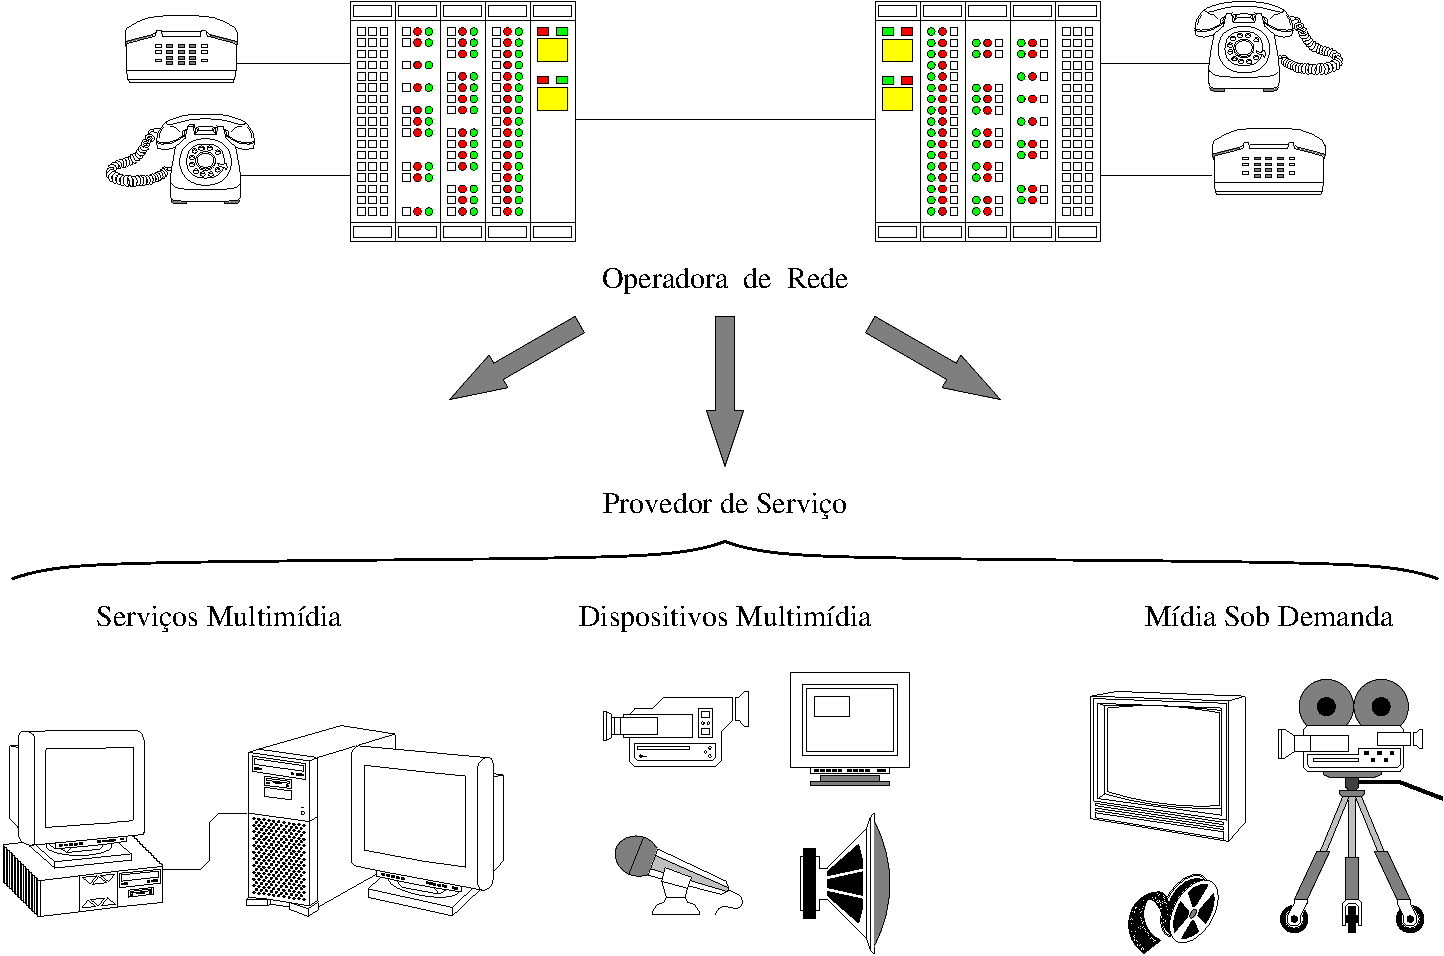
\includegraphics[width=\textwidth]{./CapituloExemplo/figura1}%% Dimensões e localização
%\fonte{\citet{Larsson2003}.}%% Fonte (quando criado pelo autor, usar Autoria Própria)
%\end{figure}

%% Classe e opções de documento
\documentclass[%% Opções
%% -- Opções da classe MEMOIR --
  12pt,%% Tamanho da fonte: 10pt, 11pt, 12pt, etc.
  a4paper,%% Tamanho do papel: a4paper (A4), letterpaper (carta), etc.
  % fleqn,%% Alinhamento das equações à esquerda (comente para alinhamento centralizado)
  % leqno,%% Numeração das equações no lado esquerdo (comente para lado direito)
  oneside,%% IMPRESSÃO dos elementos textuais e pós-textuais: oneside (apenas no anverso) ou twoside (anverso e verso, se mais de 100 p.) (insere páginas em branco).
%%  
%% -- Opções da classe ABNTEX2 --
  sumario = abnt-6027-2012,%% Formatação do sumário: tradicional (estilo tradicional) ou abnt-6027-2012 (norma ABNT 6027-2012)
  chapter = TITLE,%% Títulos de capítulos em maiúsculas (comente para desabilitar)
  section = TITLE,%% Títulos de seções secundárias em maiúsculas (comente para desabilitar)
  % subsection = TITLE,%% Títulos de seções terciárias em maiúsculas (comente para desabilitar)
  % subsubsection = TITLE,%% Títulos de seções quartenárias em maiúsculas (comente para desabilitar)
%%  
%% -- Opções da classe UTFPRCT-TEX --
  pretextualoneside,%% Impressão dos elementos pré-textuais: pretextualoneside (anverso) ou pretextualtwoside (anverso e verso)
  fontetimes,%% Fonte do texto: fontetimes (times), fontearial (arial) ou fontecourier (courier), fontemodern (lmodern - default latex). Times and Arial are ABNT recommended
   %vinculoscoloridos,%% Cores nos vínculos (citações, arquivos, links, url, etc.) (comente para desabilitar). NBR 14724/2011: cor preta (inclusive hyperlinks)
  semrecuonosumario,%% Remoção do recuo dos itens no sumário (comente para adição do recuo, se estilo tradicional)
  %inserirbackref,%% Inserir backref na lista de referências (e.g., Citado na página...)
  usemakeindex,%% Compilação de glossários e índices utilizando makeindex (comente para desabilitar)
  legendascentralizadas,%% Alinhamento das legendas centralizado (comente para alinhamento à esquerda)
%%  
%% -- Opções da folha de aprovação -- 
%% O mais comum é anexar o PDF do termo de aprovação sem assinaturas. As opções abaixo são para o formato da pós-graduação UTFPR-PG (Ponta Grossa) e podem servir de placeholder para este template.
  %aprovacaoestiloppg,%% Folha de aprovação do programa de pós-graduação no estilo do PPG (comente para estilo padrão)
  %pardeassinaturas,%% Assinaturas na folha de aprovação em até duas colunas (comente para em uma única coluna)
  % linhasdeassinaturas,%% Linhas de assinaturas na folha de aprovação (comente para remover as linhas)
%%  
%% -- Opções do pacote babel (hifenização) -- % 
  %french,%% Idioma adicional para hifenização (suporte parcial)
  %spanish,%% Idioma adicional para hifenização (suporte parcial)
  %english,%% Idioma adicional para hifenização  (colocar em último para doc. em inglês)
  brazil,%% Idioma principal do documento (último da lista)    
]{utfprct}%% Classe utfprct

%%%%%%%%
% Documento em Inglês: colocar o "english" como último idioma carregado no documentclass, sendo o último a língua principal do documento.
%%%%%%%%

%%%%%%%%
%% Configuração dos avisos (warnings)
%% Comportamento do Tex quando um PDF é incluído e possui uma versão mais nova que a versão mínima especificada em \pdfminorversion. Opções: -1 (no info), 0 (default, warning), 1 (error)
\pdfinclusionerrorlevel=-1%no warning 
%\pdfminorversion=5%pdf minor output version (default 5)

%% [Badbox] Underfull e Overfull nível de aviso (filtra o que está abaixo)
\hbadness=5000%0 até 10000 (max) nível de badness
\vbadness=1000%0 até 10000 (max) nível de badness
%\hfuzz=0.01pt%excesso permitido de largura (\hbox)para ser considerado overfull
%\vfuzz=0.001pt%excesso permitido de altura (\vbox) para ser considerado overfull
%\overfullrule=10mm%adicionar aviso visual para um badbox
%%%%%%%%

%%%%%%%%
%% Pacotes carregados nas classes:
%%   memoir: abstract, appendix, array, booktabs, ccaption, chngcntr, chngpage, dcolumn, delarray, enumerate, epigraph, framed, ifmtarg, ifpdf, index, makeidx, moreverb, needspace, newfile, nextpage, parskip, patchcmd, setspace, shortvrb, showidx, tabularx, titleref, titling, tocbibind, tocloft, verbatim, verse.
%%   memoir (similares): crop, fancyhdr, geometry, sidecap, subfigure, titlesec.
%%   abntex2: babel, bookmark, calc, enumitem, ifthen, hyperref, textcase.
%%   utfprct: abntex2cite, ae, algorithmic, amsmath, backref, breakurl, caption, subcaption, cmap, color, eepic, epic, epsfig, etoolbox, fancyhdr, fix-cm, fontenc, glossaries, graphics, graphicx, helvet, hyphenat, indentfirst, inputenc, lastpage, morewrites, nomencl, sfmath, sistyle, substr, times, xtab, pdfpages.

%% Pacotes adicionais (\usepackage[options]{package})
\usepackage{bigdelim, booktabs, colortbl, longtable, multirow}%% Ferramentas para tabelas
\usepackage{amssymb, amstext, amsthm, icomma}%% Ferramentas para linguagem matemática
\usepackage{pifont, textcomp, wasysym}%% Símbolos de texto

%%%% By Luders
\newcommand{\ric}[1]{\textcolor{blue}{#1}}
%\usepackage{subfig}

%%%% By Alt
\newcommand{\alt}[1]{\textcolor{green}{#1}}

% Refinamento tipográfico: diminui badboxes
\usepackage{microtype}%

%% Comandos personalizados (\newcommand{name}[num]{definition})
\newcommand{\cpp}{\texttt{C$++$}}%% C++
\newcommand{\latex}{\LaTeX}%% LaTeX
\newcommand{\ds}{\displaystyle}%% Tamanho normal das equações
\newcommand{\bsym}[1]{\boldsymbol{#1}}%% Texto no modo matemático em negrito
\newcommand{\mr}[1]{\mathrm{#1}}%% Texto no modo matemático normal (não itálico)
\newcommand{\der}{\mr{d}}%% Operador diferencial
\newcommand{\deri}[2]{\frac{\der#1}{\der#2}}%% Derivada ordinária
\newcommand{\derip}[2]{\frac{\partial#1}{\partial#2}}%% Derivada parcial
\newcommand{\pare}[1]{\left(#1\right)}%% Parênteses
\newcommand{\colc}[1]{\left[#1\right]}%% Colchetes
\newcommand{\chav}[1]{\left\lbrace#1\right\rbrace}%% Chaves
\newcommand{\sen}{\operatorname{sen}}%% Operador seno
\newcommand{\senh}{\operatorname{senh}}%% Operador seno hiperbólico
\newcommand{\tg}{\operatorname{tg}}%% Operador tangente
\newcommand{\tgh}{\operatorname{tgh}}%% Operador tangente hiperbólico  
\ifthenelse{\equal{\languagename}{english}}{%%
\newcommand{\nomeequacao}{Equation}
\newcommand{\nomeequacoes}{Equations}
}{%default pt
\newcommand{\nomeequacao}{Equação}
\newcommand{\nomeequacoes}{Equações}
}%  
\newcommand{\seqref}[1]{\nomeequacao~\eqref{#1}}%% Referência de uma única equação
\newcommand{\meqref}[1]{\nomeequacoes~\eqref{#1}}%% Referência de multiplas equações
\newcommand{\citep}[1]{\cite{#1}}%% Atalho para citação implícita
\newcommand{\citet}[1]{\citeonline{#1}}%% Atalho para citação explícita
\newcommand{\citepa}[1]{(\citeauthor{#1})}%% Atalho para citação implícita (somente autor)
\newcommand{\citeta}[1]{\citeauthoronline{#1}}%% Atalho para citação explícita (somente autor)
\newcommand{\citepy}[1]{(\citeyear{#1})}%% Atalho para citação implícita (somente ano)
\newcommand{\citety}[1]{\citeyear{#1}}%% Atalho para citação explícita (somente ano)

%allow fixed size on collums with text position
\newcolumntype{L}[1]{>{\raggedright\let\newline\\\arraybackslash\hspace{0pt}}m{#1}}
\newcolumntype{C}[1]{>{\centering\let\newline\\\arraybackslash\hspace{0pt}}m{#1}}
\newcolumntype{R}[1]{>{\raggedleft\let\newline\\\arraybackslash\hspace{0pt}}m{#1}}

%%%%%%%%%%%%%%%%%%%%%%%%%%%%%%%%%%%%%%%%%%%%%%%
%%%%%%%%%%%%%%%%%%%%%%%%%%%%%%%%%%%%%%%%%%%%%%%
%% Configuração das entradas
%%

%% Arquivo de dados do modelo de documento LaTeX para produção de trabalhos acadêmicos da UTFPR
%% UTFPRCT-TEX, v1.0.1 wmeira on 2020/06/06
%% Copyright (C) 2020- by William H. T. Meira
%%
%% Modified version of project 'utfprpgtex' maintained 
%% by Luiz E. M. Lima
%%
%% This work may be distributed and/or modified under the
%% conditions of the LaTeX Project Public License, either version 1.3
%% of this license or (at your option) any later version.
%% The latest version of this license is in
%%   http://www.latex-project.org/lppl.txt
%% and version 1.3 or later is part of all distributions of LaTeX
%% version 2005/12/01 or later.
%%
%% This work has the LPPL maintenance status `maintained'.
%%
%% The Current Maintainer of this work is William H. T. Meira.
%%
%% This project consists mainly of files: 'utfprct.cls', 'utfprct.tex', 
%% 'utfprct-dados.tex' 
%% 
%% The 'abntex2-alf.bst' and 'abntex2-num.bst' files are slightly
%% modified versions of the bibtex styles from abntex2 (v.1.9.7)
%% package to suit NBR6023/2018 (not yet implemented there). 
%% Complementary, 'abntex2-alf-en.bst' and 'abntex2-num-en.bst' are
%% english versions of the respective bibtex styles.
%%
%% Contribute to improve this project (github repo):
%% https://github.com/wmeira/utfprct-tex

%%%%%%%%%%%%%%%%%%%%%%%%%%%%%%%%%%%%%%%%%%%%%%%
%%%%%%%%%%%%%%%%%%%%%%%%%%%%%%%%%%%%%%%%%%%%%%%
%% Tutorial do Documento de Dados 
%%%%%%%%%%%%%%%%%%%%%%%%%%%%%%%%%%%%%%%%%%%%%%%
%%
%% O 'utfprct-dados.tex' contém todos as informações do documento, 
%% metadados e outros valores importantes para o preenchimento dos 
%% elementos pré-textuais: capa, folha de rosto, resumo, abstract.
%% 
%% Não é necessário preencher todos os campos, existem campos mais
%% específicos para o tipo de documento sendo elaborado. Quando TCC,
%% por exemplo, não é necessário definir dados do programa de 
%% pós-graduação. Todos os dados inseridos estarão disponíveis para
%% inserção no tex usando o padrão '\imprimir + nomedodadominusculo'. 
%% Por exemplo, para imprimir o tipo do documento ('\TipoDeDocumento'),
%% usar '\imprimirtipodedocumento'.
%%
%% É possível customizar a descrição do documento na folha de rosto. 
%% Exemplos de descrição são fornecidos para guiar a escrita do texto,
%% em que pode-se utilizar os dados já definidos com o padrão descrito.
%%
%% Existe a possibilidade de inserir dados de uma instituição de 
%% cotutela quando se aplicar. 
%%
%% Os dados da ficha catalográfica são fornecidos pela biblioteca
%% e, na maioria das vezes, apenas anexa-se a folha digitalizada
%% na região definida dos elementos pré-textuais.
%%
%% A folha de aprovação é, na maioria das vezes, fornecido 
%% digitalmente pelo departamento ou pelo orientador após a defesa e 
%% deverá ser anexada ao documento na região definida dos elementos 
%% pré-textuais. Recomenda-se apenas anexar a folha de aprovação sem
%% precisar alterar os dados específicos aqui presentes, pois foram
%% criados originalmente para o template da folha de aprovação da
%% UTFPR-PG, presente no projeto base, e foram apenas mantidos.
%%
%%%%%%%%%%%%%%%%%%%%%%%%%%%%%%%%%%%%%%%%%%%%%%%
%%%%%%%%%%%%%%%%%%%%%%%%%%%%%%%%%%%%%%%%%%%%%%%

%%%%%%%%%%%%%%%%%%%%%%%%%%%%%%%%%%%%%%%%%%%%%%%
%% Informações do Documento
%%%%%%%%%%%%%%%%%%%%%%%%%%%%%%%%%%%%%%%%%%%%%%%

%% Tipo de documento (opções: "Tese", "Dissertação", "Trabalho de Conclusão de Curso"
\TipoDeDocumento{Dissertação}%copiar exatamente uma das opções 

%% [abstract] Document type: "Thesis", "Dissertation", "Bachelor Thesis"
\DocumentType{Dissertation}%

%% Nível de formação: "Doutorado", "Mestrado", "Bacharelado"
\NivelDeFormacao{Mestrado}%

%% [abstract] Formation level: "Doctorate", "PhD", "Master's Degree", "Bachelor's Degree"
\FormationLevel{Master's Degree}%

%% Título pretendido: "Doutor(a)", "Mestre(a)" ou "Bacharel(a)"
\TituloPretendido{Mestre}%

%% Título do documento
\TituloDoDocumento{%%
Grafos Temporais com Neo4j
}%

%% [abstract] Document title
\DocumentTitle{%%
Title of this academic work: subtitle of this academic work
}%

%% Título em múltiplas linhas na capa, folha de rosto e termo de aprovação
%% Use o comando \par para indicar a quebra de linha
\TituloEmMultiplasLinhas{%%
% Título do presente trabalho acadêmico: \par 
% subtítulo do presente trabalho acadêmico
Grafos Temporais com Neo4j
}%

%% Data da defesa
\Dia{1}%% Dia (opcional: usado na ficha catalográfica apenas)
\MesPorExtenso{janeiro}%% mês por extenso (opcional: usado na ficha catalográfica apenas)
\Ano{2020}%% Ano

%% Palavras-chave e keywords (máximo 5)
\NumeroDePalavrasChave{5}%% Número de palavras-chave 
\PalavraChaveA{Palavra-chave A}%% Palavra-chave A
\PalavraChaveB{Palavra-chave B}%% Palavra-chave B
\PalavraChaveC{Palavra-chave C}%% Palavra-chave C
\PalavraChaveD{Palavra-chave D}%% Palavra-chave D
\PalavraChaveE{Palavra-chave E}%% Palavra-chave E

\NumeroDeKeywords{\imprimirnumerodepalavraschave}%% Número de keywords (mesmo que palavras-chave)
\KeywordA{Keyword A}%% Keyword A
\KeywordB{Keyword B}%% Keyword B
\KeywordC{Keyword C}%% Keyword C
\KeywordD{Keyword D}%% Keyword D
\KeywordE{Keyword E}%% Keyword E

%%%%%%%%%%%%%%%%%%%%%%%%%%%%%%%%%%%%%%%%%%%%%%%
%% Informação do Autor(a) ou Autores(as) (TCC)
%%%%%%%%%%%%%%%%%%%%%%%%%%%%%%%%%%%%%%%%%%%%%%%

%%% Autor(a)
%% Usado para citação: "\SobrenomeDoAutor, PrenomeDoAutor" (ex: "Doe, John" ou "Doe, J.")
\NomeDoAutor{Altieris Marcelino Peixoto}%% Nome completo do(a) autor(a)
\SobrenomeDoAutor{Peixoto}%% Último nome do(a) autor(a)
\PrenomeDoAutor{Altieris Marcelino}%% Nome do(a) autor(a) sem último nome

%%% Autor(a) 2 (opcional)
%% *Considera apenas se "\TipoDeDocumento" == "Trabalho de Conclusão de Curso"
\AtribuiAutorDois{false}%% Insere ou remove autor(a) 2: "true" ou "false"
\NomeDoAutorDois{Nome do(a) Autor(a) 2}%% Nome completo do(a) autor(a) 2
\SobrenomeDoAutorDois{Último Nome}%% Último nome do(a) autor(a) 2
\PrenomeDoAutorDois{Nome do(a) Autor(a) 2 Sem Último}%% Nome do(a) autor(a) 2 sem último nome

%%% Autor(a) 3 (opcional)
%% *Considera apenas se "\TipoDeDocumento" == "Trabalho de Conclusão de Curso"
\AtribuiAutorTres{false}%% Insere ou remove autor(a) 3: "true" ou "false"
\NomeDoAutorTres{Nome do(a) Autor(a) 3}%% Nome completo do(a) autor(a) 3
\SobrenomeDoAutorTres{Último Nome}%% Último nome do(a) autor(a) 3
\PrenomeDoAutorTres{Nome do(a) Autor(a) 3 Sem Último}%% Nome do(a) autor(a) 3 sem último nome

%%%%%%%%%%%%%%%%%%%%%%%%%%%%%%%%%%%%%%%%%%%%%%%%%%
%% Informações do Orientador(a) e Coorientador(a)
%%%%%%%%%%%%%%%%%%%%%%%%%%%%%%%%%%%%%%%%%%%%%%%%%%

%% Orientador(a)
%% Usado para citação: "\SobrenomeDoOrientador, PrenomeDoOrientador" (ex: "Doe, John" ou "Doe, J.")
\AtribuicaoOrientador{Ricardo Lüders}%% Atribuição "Orientador(a)"
\TituloDoOrientador{Prof(a). Dr(a).}%% Título do(a) orientador(a)
\NomeDoOrientador{Nome Completo do(a) Orientador(a)}%% Nome completo do(a) orientador(a)
\SobrenomeDoOrienador{Último Nome}%% Último nome do(a) orientador(a)
\PrenomeDoOrientador{Nome do(a) Orientador(a) Sem Último}%% Nome do(a) orientador(a) sem último nome

%% Coorientador(a) (opcional)
%% Usado para citação: "\SobrenomeDoCoorientador, PrenomeDoCoorientador" (ex: "Doe, John" ou "Doe, J.")
\AtribuiCoorientador{true}%% Insere ou remove o(a) coorientador(a): "true" ou "false"
\AtribuicaoCoorientador{Coorientador(a)}%% Atribuição "Coorientador(a)"
\TituloDoCoorientador{Prof(a). Dr(a).}%% Título do(a) coorientador(a)
\NomeDoCoorientador{Nome Completo do(a) Coorientador(a)}%% Nome completo do(a) coorientador(a)
\SobrenomeDoCoorienador{Último Nome}%% Último nome do(a) coorientador(a)
\PrenomeDoCoorientador{Nome do(a) Coorientador(a) Sem Último}%% Nome do(a) coorientador(a) sem último nome

%%%%%%%%%%%%%%%%%%%%%%%%%%%%%%%%%%%%%%%%%%%%%%%%%%
%% Informações da Instituição
%%%%%%%%%%%%%%%%%%%%%%%%%%%%%%%%%%%%%%%%%%%%%%%%%%

%% Nome da instituição
\Instituicao{Universidade Tecnológica Federal do Paraná}

%% [abstract] Institution name (*nome sem traduzir é o recomendado para docs. da UTFPR)
\Institution{Universidade Tecnológica Federal do Paraná}

%% Sigla da Instituição
\SiglaInstituicao{UTFPR}

%% Nome da cidade (câmpus)
\Cidade{Curitiba}

%% Diretoria: "Graduação e Educação Profissional" ou "Pesquisa e Pós-Graduação" (opcional)
\Diretoria{Pesquisa e Pós-Graduação}

%% Nome do departamento ou da coordenação (opcional: mais comum no Bacharelado: Departamento de Informática)
\Departamento{Nome do Departamento ou da Coordenação}

%% Sigla do departamento (opcional, ex: DAINF, DAMEC, DAMAT...)
\SiglaDepartamento{DPT}

%% Nome do curso bachalerado ou pós-graduação (PPG) (ex: "Engenharia de Computação",  "Engenharia El{\'e}trica e Inform{\'a}tica Industrial") 
\Curso{Engenharia El{\'e}trica e Inform{\'a}tica Industrial}

%% [abstract] Course name
\Course{Course Name}

%% Programa ou nome do curso completo (capa)
%% "Bachalerado em Engenharia de Computação"
%% "Programa de Pós-Graduação em Engenharia Elétrica e Informática Industrial"
\Programa{Programa de Pós-Graduação em \imprimircurso}

%% Sigla do programa de pós-graduação (opcional, ex: CPGEI, PPGCA)
\SiglaDoPPG{PPG}

%% Nome da área de concentração
\AreaDeConcentracao{Engenharia de Computação}

%%%%%%%%%%%%%%%%%%%%%%%%%%%%%%%%%%%%%%%%%%%%%%%%%%%%%%
%% Informações de Cotutela (Duplo Grau) (opcional)
%%%%%%%%%%%%%%%%%%%%%%%%%%%%%%%%%%%%%%%%%%%%%%%%%%%%%%

%% Insere dados de cotutela: "true" ou "false"
\AtribuiCotutela{false}

%% Nome da instituição de cotutela
\InstituicaoCotutela{Universidade Da Cotutela}

%% [abstract] Institution name
\InstitutionCotutela{Double Degree University}

%% Sigla da instituição de cotutela
\SiglaInstituicaoCotutela{UC}

%% Nome do departamento ou da coordenação da inst. de cotutela (mais comum no Bacharelado: Departamento de Informática)
\DepartamentoCotutela{Nome do Departamento ou da Coordenação}

%% Sigla do departamento da inst. cotutela (ex: DAINF, DAMEC, DAMAT...)
\SiglaDepartamentoCotutela{DPT-EXT}

%% Nome do curso bachalerado ou pós-graduação (PPG) na instituição de cotutela (ex: "Engenharia de Computação",  "Engenharia El{\'e}trica e Inform{\'a}tica Industrial")
\CursoCotutela{Nome do Curso Cotutela}

%% [abstract] Course name 
\CourseCotutela{Second Degree Course}

%% Programa ou nome do curso completo na inst. cotutela (capa)
%% "Bachalerado em Engenharia de Computação"
%% "Programa de Pós-Graduação em Engenharia Elétrica e Informática Industrial"
\ProgramaCotutela{Programa de Doutoral em \imprimircursocotutela}

%% Sigla do programa externo de pós-graduação
\SiglaDoPPGCotutela{PPG-EXT}

%% Nome da área de concentração na instituição de cotutela
\AreaDeConcentracaoCotutela{Nome da Área de Concentração}

%% Nível de formação que será fornecido na referência do doc.
\NivelDeFormacaoResumo{Duplo doutorado}
\FormationLevelAbstract{Double PhD}

%% Informacoes do orientador(a) na instituição de cotutela

%% Orientador(a) da instituição de cotutela
%% Usado para citação: "\SobrenomeDoOrientador, PrenomeDoOrientador" (ex: "Doe, John" ou "Doe, J.")
\AtribuicaoOrientadorCotutela{Orientador(a)}%% Atribuição "Orientador(a)"
\TituloDoOrientadorCotutela{Prof(a). Dr(a).}%% Título do(a) orientador(a)
\NomeDoOrientadorCotutela{Nome Completo do(a) Orientador(a)}%% Nome completo do(a) orientador(a)
\SobrenomeDoOrienadorCotutela{Último Nome}%% Último nome do(a) orientador(a)
\PrenomeDoOrientadorCotutela{Nome do(a) Orientador(a) Sem Último}%% Nome do(a) orientador(a) sem último nome

%% Coorientador(a) da instituição de cotutela
%% Usado para citação: "\SobrenomeDoCoorientador, PrenomeDoCoorientador" (ex: "Doe, John" ou "Doe, J.")
\AtribuiCoorientadorCotutela{false}%% Insere ou remove o(a) coorientador(a) da cotutela: "true" ou "false"
\AtribuicaoCoorientadorCotutela{Coorientador(a)}%% Atribuição "Coorientador(a)"
\TituloDoCoorientadorCotutela{Prof(a). Dr(a).}%% Título do(a) coorientador(a)
\NomeDoCoorientadorCotutela{Nome Completo do(a) Coorientador(a)}%% Nome completo do(a) coorientador(a)
\SobrenomeDoCoorienadorCotutela{Último Nome}%% Último nome do(a) coorientador(a)
\PrenomeDoCoorientadorCotutela{Nome do(a) Coorientador(a) Sem Último}%% Nome do(a) coorientador(a) sem último nome

%%%%%%%%%%%%%%%%%%%%%%%%%%%%%%%%%%%%%%%%%%%%%%%%%%
%% Folha de Rosto
%%%%%%%%%%%%%%%%%%%%%%%%%%%%%%%%%%%%%%%%%%%%%%%%%%

%% Se desejar usar os dados inseridos, eles estão disponíves
%% usando o padrão '\imprimir + nomedodadominusculo'. Por exemplo,
%% para imprimir o tipo do documento ('\TipoDeDocumento'), usar
%% '\imprimirtipodedocumento'

%% Descrição do documento na folha de rosto (exemplos)
\DescricaoDoDocumento{
%\imprimirtipodedocumento\ apresentada ao Programa de Pós-Graduação em \imprimircurso\ (\imprimirsigladoppg) da \imprimirinstituicao\ (\imprimirsiglainstituicao)\ como requisito à obtenção do título de ``Doutor em Ciências''. Área de Concentração: \imprimirareadeconcentracao.%
\imprimirtipodedocumento\ apresentado(a) como requisito parcial à obtenção do título de \imprimirtitulopretendido\ em \imprimircurso, do \imprimirppgoudepartamento, da \imprimirinstituicao.
}

%% Insere ou remove descrição da cotutela (extra) na folha de rosto: "true" ou "false". 
%% Se "true", a descrição do documento será colocada na folha de rosto, logo abaixo do orientador(a) e coorientador(a) da primeira inst. e depois o orientador(a) e coorientador(a) da inst. de cotutela. 
%% Se "false", os nomes do orientador(a) e coorientador(a) aparecerão logo abaixo do orientador(a) da primeira instituição, sem uma descrição extra. Neste caso, recomenda-se revisar a "\DescricaoDoDocumento" para contemplar ambas as instituições.   
\AtribuiDescricaoCotutela{false}

%% Segunda Descricao da Inst. de Cotutela na folha de rosto (exemplos)
\DescricaoDoDocumentoCotutela{
\imprimirtipodedocumento\ apresentado(a) como requisito parcial à obtenção do título de \imprimirtitulopretendido\ em \imprimircursocotutela, do \imprimirppgoudepartamentocotutela, da \imprimirinstituicaocotutela.  
%\imprimirtipodedocumento\ apresentada à Comissão de Acompanhamento de Tese do Programa Doutoral em \imprimircursocotutela\ do \imprimirinstituicaocotutela\ (\imprimirsiglainstituicaocotutela) como requisito à obtenção de grau de \imprimirtitulopretendido\ na área de concentração \imprimirareadeconcentracaocotutela.
}

%%%%%%%%%%%%%%%%%%%%%%%%%%%%%%%%%%%%%%%%%%%%%%%%%%
%% Ficha Catalográfica* (opcional)
%%%%%%%%%%%%%%%%%%%%%%%%%%%%%%%%%%%%%%%%%%%%%%%%%%

%% *Pode ser usado como placeholder, porém para entrega deve-se inserir a ficha catolográfica digitalizado (PDF) pela biblioteca da UTFPR.

\NumeroDaPublicacao{00/\imprimirano}%% Número da publicação - Fornecido pela biblioteca
\CDDOuCDU{CDD 000.00}%% Classificação Decimal Dewey (CDD) ou Classificação Decimal Universal (CDU) - Fornecida pela biblioteca

\TituloDaFichaCatalografica{%% Título da ficha catalográfica
  Ficha catalográfica elaborada pelo Departamento de Biblioteca da \par \imprimirinstituicao, Câmpus \imprimircidade \par n.
  \imprimirnumerodapublicacao
}

%%%%%%%%%%%%%%%%%%%%%%%%%%%%%%%%%%%%%%%%%%%%%%%%%%
%% Folha de aprovação (Formato UTFPR-PG)* (opcional)
%%%%%%%%%%%%%%%%%%%%%%%%%%%%%%%%%%%%%%%%%%%%%%%%%%

%% *Pode ser usado como placeholder, porém para entrega final prefere-se a folha (termo) de aprovação digitalizado (PDF) fornecido pelo departamento ou orientador.

\NumeroDaTeseOuDissertacao{00/\imprimirano}%% Número da Tese ou Dissertação - Fornecido pelo programa de pós-graduação
\NumeroDaFichaCatalografica{A000}%% Número da ficha catalográfica - Fornecido pela biblioteca

\TituloDoResponsavelTCC{Prof(a). Dr(a).}%% Título do(a) responsável pelos TCC
\NomeDoResponsavelTCC{Nome do(a) Responsável}%% Nome completo do(a) responsável pelos TCC
\AtribuicaoCoordenador{Coordenador(a)}%% Atribuição "Coordenador(a)" do curso
\TituloDoCoordenador{Prof(a). Dr(a).}%% Título do(a) coordenador(a) do curso
\NomeDoCoordenador{Nome do(a) Coordenador(a)}%% Nome completo do(a) coordenador(a) do curso

\TextoDeAprovacao{%% Texto de aprovação
  %% Exemplo de texto de aprovação para Tese ou Dissertação (descomente a próxima linha para utilizá-lo):
  Esta \imprimirtipodedocumento\ foi apresentada às 00:00 de \imprimirdia\ de \imprimirmesporextenso\ de \imprimirano\ como requisito parcial para a obtenção do título de \imprimirtitulopretendido\ em \imprimircurso, na área de concentração em \imprimirareadeconcentracao\ e na linha de pesquisa em (Nome da Linha de Pesquisa), do Programa de Pós-Graduação em \imprimircurso. O(A) candidato(a) foi arguido(a) pela Banca Examinadora composta pelos professores abaixo citados. Após deliberação, a Banca Examinadora considerou o trabalho aprovado.
  %% Exemplo de texto de aprovação para Trabalho de Conclusão de Curso (descomente a próxima linha para utilizá-lo):
  % Este \imprimirtipodedocumento\ foi apresentado em \imprimirdia\ de \imprimirmesporextenso\ de \imprimirano\ como requisito parcial para a obtenção do título de \imprimirtitulopretendido\ em \imprimircurso. O(A) candidato(a) foi arguido(a) pela Banca Examinadora composta pelos professores abaixo assinados. Após deliberação, a Banca Examinadora considerou o trabalho aprovado.
}

\AvisoDeAprovacao{%% Aviso de aprovação
  %% Exemplo de aviso de aprovação para Tese ou Dissertação (descomente a próxima linha para utilizá-lo):
  A Folha de Aprovação assinada encontra-se no \par Departamento de Registros Acadêmicos da UTFPR -- Câmpus \imprimircidade
  %% Exemplo de aviso de aprovação para Trabalho de Conclusão de Curso (descomente a próxima linha para utilizá-lo):
  % -- O Termo de Aprovação assinado encontra-se na Coordenação do Curso --
}

%% Banca examinadora: 3 membros (Trabalho de Conclusão de Curso ou Dissertação); 5 a 7 membros (Tese)
\MembroAIgualOrientador{true}%% Insere ou remove o membro A igual ao(à) orientador(a): "true" ou "false"
\MembroA{Nome do Membro A}%% Nome completo do membro A - Presidente (automático se orientador(a))
\TituloDoMembroA{Prof(a). Dr(a).}%% Título do membro A - Presidente (automático se orientador(a))
\InstituicaoDoMembroA{Instituição do Membro A}%% Nome da instituição do membro A - Presidente (automático se orientador(a))
\MembroB{Nome do Membro B}%% Nome completo do membro B
\TituloDoMembroB{Prof(a). Dr(a).}%% Título do membro B
\InstituicaoDoMembroB{Instituição do Membro B}%% Nome da instituição do membro B
\MembroC{Nome do Membro C}%% Nome completo do membro C
\TituloDoMembroC{Prof(a). Dr(a).}%% Título do membro C
\InstituicaoDoMembroC{Instituição do Membro C}%% Nome da instituição do membro C
\MembroD{Nome do Membro D}%% Nome completo do membro D
\TituloDoMembroD{Prof(a). Dr(a).}%% Título do membro D
\InstituicaoDoMembroD{Instituição do Membro D}%% Nome da instituição do membro D
\MembroE{Nome do Membro E}%% Nome completo do membro E
\TituloDoMembroE{Prof(a). Dr(a).}%% Título do membro E
\InstituicaoDoMembroE{Instituição do Membro E}%% Nome da instituição do membro E
\AtribuiMembroF{false}%% Insere ou remove o Membro F: "true" ou "false"
\MembroF{Nome do Membro F}%% Nome completo do membro F
\TituloDoMembroF{Prof(a). Dr(a).}%% Título do membro F
\InstituicaoDoMembroF{Instituição do Membro F}%% Nome da instituição do membro F
\AtribuiMembroG{false}%% Insere ou remove o Membro G: "true" ou "false"
\MembroG{Nome do Membro G}%% Nome completo do membro G
\TituloDoMembroG{Prof(a). Dr(a).}%% Título do membro G
\InstituicaoDoMembroG{Instituição do Membro G}%% Nome da instituição do membro G%% Realize as modificações pertinentes no arquivo "utfprct-dados.tex"

%% Ferramenta para criação de índices
\makeindex%% Não comente esta linha

%% Ferramenta para criação de glossários
\makeglossaries%% Não comente esta linha

%% Entradas da lista de abreviaturas, siglas e acrônimos
% %%%% LISTA DE ABREVIATURAS, SIGLAS E ACRÔNIMOS
%%
%% Relação, em ordem alfabética, das abreviaturas (representação de uma palavra por meio de alguma(s) de sua(s) sílaba(s) ou
%% letra(s)), siglas (conjunto de letras iniciais dos vocábulos e/ou números que representa um determinado nome) e acrônimos
%% (conjunto de letras iniciais dos vocábulos e/ou números que representa um determinado nome, formando uma palavra pronunciável).
%%
%%
%% Este arquivo para definição de abreviaturas, siglas e acrônimos é utilizado com a opção \incluirlistadeacronimos{glossaries}
%%
%% Vantagens do modo com "glossaries" em relação ao modo "file":
%%   1) Ordena automaticamente a lista
%%	 2) Apenas os termos referenciados são colocados na lista


%% Como referenciar: 
%% \gls{lp} = Linear Programming (LP)  (First use)
%% \gls{lp} = LP (Next uses)
%% \glspl{lp} = LPs
%% \glsentrytext{lp} = Linear Programming    (recommended for chapter/section/....)
%% \glsentrylong{lp} = Linear Programming
%% \glsentryshort{lp} = LP

%% Para acrônimos também funciona:  
%% \acrlong{lp} = Linear Programming
%% \acrshort{lp} = LP

%% Abreviaturas: \abreviatura{rótulo}{representação}{definição}

\abreviatura{art.}{art.}{Artigo}
\abreviatura{cap.}{cap.}{Capítulo}
\abreviatura{sec.}{sec.}{Seção}

%% Siglas: \sigla{rótulo}{representação}{definição}

\sigla{abnt}{ABNT}{Associação Brasileira de Normas Técnicas}
\sigla{cnpq}{CNPq}{Conselho Nacional de Desenvolvimento Científico e Tecnológico}
\sigla{eps}{EPS}{\textit{Encapsulated PostScript}}
\sigla{pdf}{PDF}{Formato de Documento Portátil, do inglês \textit{Portable Document Format}}
\sigla{ps}{PS}{\textit{PostScript}}
\sigla{utfpr}{UTFPR}{Universidade Tecnológica Federal do Paraná}

%% Acrônimos: \acronimo{rótulo}{representação}{definição}

\acronimo{gimp}{Gimp}{Programa de Manipulação de Imagem GNU, do inglês \textit{GNU Image Manipulation Program}}
% Comente para remover este item

%% Entradas do glossário
% %%%% GLOSSÁRIO
%%
%% Relação de palavras ou expressões técnicas de uso restrito ou de sentido obscuro, utilizadas no texto, acompanhadas das
%% respectivas definições.

%% Entradas do glossário: \newglossaryentry{rótulo}{informações da entrada}

\newglossaryentry{pai}{%% Informações da entrada
  name        = {pai},
  plural      = {pais},
  description = {um exemplo de entrada pai que possui subentradas (entradas filhas)}
}

\newglossaryentry{componente}{%% Informações da entrada
  name        = {componente},
  plural      = {componentes},
  parent      = {pai},
  description = {um exemplo de uma entrada componente, subentrada da entrada chamada \gls{pai}}
}

\newglossaryentry{filho}{%% Informações da entrada
  name        = {filho},
  plural      = {filhos},
  parent      = {pai},
  description = {um exemplo de uma entrada filha (subentrada) da entrada chamada \gls{pai}. Trata-se de uma entrada irmã da entrada chamada \gls{componente}}
}

\newglossaryentry{equilibrio}{%% Informações da entrada
  name        = {equilíbrio da configuração},
  see         = [veja também]{componente},
  description = {uma consistência entre os \glspl{componente}}
}

\newglossaryentry{tex}{%% Informações da entrada
  name        = {\TeX},
  sort        = {TeX},
  description = {é um sistema de tipografia criado por Donald E. Knuth}
}

\newglossaryentry{latex}{%% Informações da entrada
  name        = {\latex},
  sort        = {LaTeX},
  description = {um conjunto de macros para o processador de textos \gls{tex}, utilizado amplamente para a produção de textos matemáticos e científicos devido à sua alta qualidade tipográfica}
}

\newglossaryentry{bibtex}{%% Informações da entrada
  name        = {Bib\TeX},
  sort        = {BibTeX},
  parent      = {latex},
  description = {um software de gerenciamento de referências para a formatação de listas de referências. A ferramenta Bib\TeX\ é normalmente usada em conjunto com o sistema de preparação de documentos do \gls{latex}}
}

\newglossaryentry{abntex2}{%% Informações da entrada
  name        = {\abnTeX},
  sort        = {abnTeX2},
  see         = {latex},
  description = {uma suíte para \gls{latex} que atende os requisitos das normas da Associação Brasileira de Normas Técnicas (ABNT) para elaboração de documentos técnicos e científicos brasileiros, como artigos científicos, relatórios técnicos, trabalhos acadêmicos como teses, dissertações, projetos de pesquisa e outros documentos do gênero}
}

\newglossaryentry{utfprpgtex}{%% Informações da entrada
  name        = {\utfprpgtex},
  sort        = {UTFPRPGTeX},
  see         = {latex},
  parent      = {abntex2},
  description = {uma suíte para \gls{latex}, baseada na suíte \gls{abntex2}, que atende os requisitos das normas definidas pela Universidade Tecnológica Federal do Paraná (UTFPR), câmpus Ponta Grossa, para elaboração de trabalhos acadêmicos}
}

\newglossaryentry{utfprcttex}{%% Informações da entrada
  name        = {\utfprcttex},
  sort        = {UTFPRCTTeX},
  see         = {latex},
  parent      = {abntex2},
  description = {uma suíte para \gls{latex}, baseada na suíte \gls{abntex2}, que atende os requisitos das normas definidas pela Universidade Tecnológica Federal do Paraná (UTFPR), câmpus Curitiba, para elaboração de trabalhos acadêmicos}
}
% Comente para remover este item

%% Ferramenta para criação de nomenclaturas
\makenomenclature%% Não comente esta linha

%%%%%%%%%%%%%%%%%%%%%%%%%%%%%%%%%%%%%%%%%%%%%%%
%%%%%%%%%%%%%%%%%%%%%%%%%%%%%%%%%%%%%%%%%%%%%%%
%% Início do documento
%%
\begin{document}%% Não comente esta linha

%%%%%%%%%%%%%%%%%%%%%%%%%%%%%%%%%%%%%%%%%%%%%%%
%%%%%%%%%%%%%%%%%%%%%%%%%%%%%%%%%%%%%%%%%%%%%%%
%% Formatação de páginas de elementos pré-textuais
%%
\pretextual%% Não comente esta linha


%%%%%%%%%%%%%%%%%%%%%%%%%%%%%%%%%%%%%%%%%%%%%%%
%% Capa
%%
\incluircapa%% Comente para remover este item
%%%%%%%%%%%%%%%%%%%%%%%%%%%%%%%%%%%%%%%%%%%%%%%


%%%%%%%%%%%%%%%%%%%%%%%%%%%%%%%%%%%%%%%%%%%%%%%
%% Folha de rosto (comentar para remover pré-textual)
%%
%% A descrição da folha de rosto pode ser customizada no 
%% arquivo de dados ('utfprct-dados.tex) alterando o dado
%% '\DescricaoDoDocumento'.
%%
%% Comando com * coloca a ficha catalográfica no verso
%%
\incluirfolhaderosto*%% Com ficha catalográfica no verso 
%\incluirfolhaderosto%% Sem ficha catalográfica no verso
%%%%%%%%%%%%%%%%%%%%%%%%%%%%%%%%%%%%%%%%%%%%%%%


%%%%%%%%%%%%%%%%%%%%%%%%%%%%%%%%%%%%%%%%%%%%%%%
%% Ficha catalográfica (comente para remover este item)
%% A ficha catalográfica é fornecida pela biblioteca em PDF
%% e deve ser anexada no verso da folha de rosto.
%%
%% Comando \incluirfichacatalografica: 
%% 1) Aceita o path para o PDF (insere a primeira página)
%% 2) Com argumento 'template' (ou sem argumento), insere-se um template 'utfprct' (placeholder)
%%
\incluirfichacatalografica{./PreTexto/ficha_catalografica_exemplo.pdf}%%1
%\incluirfichacatalografica{template}%%2
%%%%%%%%%%%%%%%%%%%%%%%%%%%%%%%%%%%%%%%%%%%%%%%


%%%%%%%%%%%%%%%%%%%%%%%%%%%%%%%%%%%%%%%%%%%%%%%
%% Errata
% %%%% ERRATA
%%
%% Lista dos erros ocorridos no texto, seguidos das devidas correções.

%% Trocar título da errata
%\renewcommand{\nomeerrata}{Errata} %default: Errata

\begin{errata}%% Ambiente errata
\begin{table*}[htb]%% Ambiente table
\begin{tabularx}{\textwidth}{|l|l|X|X|}%% Ambiente tabularx
\toprule
\textbf{Página(s)}         & \textbf{Linha(s)} & \textbf{Onde se lê} & \textbf{Leia-se}         \\ \midrule
\pageref*{errata:capitulo} & 4, 9-11, 14-16    & capítulo(s)         & seção(ões) primária(s)   \\ \midrule
\pageref*{errata:secao}    & 12-16             & seção(ões)          & seção(ões) secundária(s) \\ \midrule
\pageref*{errata:subsecao} & 16                & subseção(ões)       & seção(ões) terciária(s)  \\ \bottomrule
\end{tabularx}
\end{table*}
\end{errata}
%% Comente para remover este item

%% Folha ou Termo de aprovação (comente para remover este item)
%% A folha de aprovação é entregue ao autor, quando aprovado, após
%% a defesa e deve ser anexada nos pré-textuais .
%% 1) Aceita o path para o PDF (insere a primeira página)
%% 2) Com argumento 'template' (ou sem argumento), insere-se um template 'utfprct', que pode servir de placeholder.
%%
\incluirfolhadeaprovacao{./PreTexto/folha_de_aprovacao_exemplo.pdf}%%1
%\incluirfolhadeaprovacao{template}%2
%%%%%%%%%%%%%%%%%%%%%%%%%%%%%%%%%%%%%%%%%%%%%%%

%%%%%%%%%%%%%%%%%%%%%%%%%%%%%%%%%%%%%%%%%%%%%%%
%% Dedicatória
%%
%%%% DEDICATÓRIA
%%
%% Texto em que o autor presta homenagem ou dedica seu trabalho.

\begin{dedicatoria}%% Ambiente dedicatoria
Dedico este trabalho a minha família e aos meus amigos, pelos momentos de ausência.
\end{dedicatoria}
%% Comente para remover este item
%%%%%%%%%%%%%%%%%%%%%%%%%%%%%%%%%%%%%%%%%%%%%%%


%%%%%%%%%%%%%%%%%%%%%%%%%%%%%%%%%%%%%%%%%%%%%%%
%% Agradecimentos
%%
%%%% AGRADECIMENTOS
%%
%% Texto em que o autor faz agradecimentos dirigidos àqueles que contribuíram de maneira relevante à elaboração do trabalho.

\begin{agradecimentos}%% Ambiente agradecimentos
%\begin{agradecimentos}[Agradecimentos]%% (opção: título do agradecimento)

Este trabalho não poderia ser terminado sem a ajuda de diversas pessoas e/ou instituições às quais presto minha homenagem. Certamente esses parágrafos não irão atender a todas as pessoas que fizeram parte dessa importante fase de minha vida. Portanto, desde já peço desculpas àquelas que não estão presentes entre estas palavras, mas elas podem estar certas que fazem parte do meu pensamento e de minha gratidão.

A minha família, pelo carinho, incentivo e total apoio em todos os momentos da minha vida.

Ao meu orientador, que me mostrou os caminhos a serem seguidos e pela confiança depositada.

A todos os professores e colegas do departamento, que ajudaram de forma direta e indireta na conclusão deste trabalho.

Enfim, a todos os que de alguma forma contribuíram para a realização deste trabalho.
\end{agradecimentos}
%% Comente para remover este item
%%%%%%%%%%%%%%%%%%%%%%%%%%%%%%%%%%%%%%%%%%%%%%%


%%%%%%%%%%%%%%%%%%%%%%%%%%%%%%%%%%%%%%%%%%%%%%%
%% Epígrafe
%%
%%%% EPÍGRAFE
%%
%% Texto em que o autor apresenta uma citação, seguida de indicação de autoria, relacionada com a matéria tratada no corpo do
%% trabalho.

\begin{epigrafe}%% Ambiente epigrafe
Primeira Lei: Um robô não pode ferir um ser humano ou, por omissão, permitir que um ser humano sofra algum mal. Segunda Lei: Um robô deve obedecer as ordens que lhe sejam dadas por seres humanos, exceto nos casos em que tais ordens contrariem a Primeira Lei. Terceira Lei: Um robô deve proteger sua própria existência desde que tal proteção não entre em conflito com a Primeira e Segunda Leis (ASIMOV, Isaac, 1950).
\end{epigrafe}
%% Comente para remover este item
%%%%%%%%%%%%%%%%%%%%%%%%%%%%%%%%%%%%%%%%%%%%%%%


%%%%%%%%%%%%%%%%%%%%%%%%%%%%%%%%%%%%%%%%%%%%%%%
%% Resumo
%%
%%%% RESUMO
%%
%% Apresentação concisa dos pontos relevantes de um texto, fornecendo uma visão rápida e clara do conteúdo e das conclusões do trabalho.

\begin{resumoutfpr}%% Ambiente resumoutfpr
O estudo das relações dinâmicas entre as estruturas topológicas de uma rede de transporte e os padrões de mobilidade nesta rede se faz importante para a criação de soluções inovadoras para problemas de confiabilidade, otimização, vulnerabilidade e previsão de tráfego. Todavia, um dos maiores desafios da área de gerência, planejamento e operação do transporte é a manipulação de um grande volume de dados, geralmente provenientes de sensores de localização instalados nos veículos. Este trabalho tem por objetivo modelar o sistema de transporte coletivo da cidade de Curitiba usando uma base de dados de grafos gerada a partir de um repositório de dados abertos com informações da operação diária do transporte. A principal contribuição é o desenvolvimento de uma plataforma computacional para a geração automática da base de grafo a partir do repositório de dados abertos. Resultados ilustrativos de diversas métricas do transporte de Curitiba são apresentados, mostrando o potencial de análise da ferramenta.

Palavras-chave. Para definição das palavras-chave (e suas correspondentes em inglês no \textit{abstract}) consultar em Termo tópico do Catálogo de Autoridades da Biblioteca Nacional, disponível em: \url{http://acervo.bn.br/sophia_web/index.html}.
\end{resumoutfpr}
%% Comente para remover este item
%%%%%%%%%%%%%%%%%%%%%%%%%%%%%%%%%%%%%%%%%%%%%%%


%%%%%%%%%%%%%%%%%%%%%%%%%%%%%%%%%%%%%%%%%%%%%%%
%% Abstract
%%
%%%% ABSTRACT
%%
%% Versão do resumo para idioma de divulgação internacional.

\begin{abstractutfpr}%% Ambiente abstractutfpr
The study of dynamic relationships between topological structures of a transport network and mobility patterns in this network is important for building smart solutions to problems of reliability, optimization, vulnerability and traffic forecast. However, one of the biggest challenge in transport planning and operation management is to deal with large volume of data often provided by geolocation sensors installed in vehicles. This work aims at modeling Curitiba transport system using a graph database built with information of daily transport operation available from an open data repository. The main contribution is the development of a computational framework for automatic building of the graph database from raw data of the repository. Illustrative results of several metrics for Curitiba transport are presented by showing the potential analysis provided by the proposed tool.

To define the keywords (and their corresponding portuguese in the \textit{resumo}) query in Authorities Catalog Topic term of the National Library, available at: \url{http://acervo.bn.br/sophia_web/index.html}.
\end{abstractutfpr}
%% Comente para remover este item
%%%%%%%%%%%%%%%%%%%%%%%%%%%%%%%%%%%%%%%%%%%%%%%

%%%%%%%%%%%%%%%%%%%%%%%%%%%%%%%%%%%%%%%%%%%%%%%
%% Lista de algoritmos
%%
% \incluirlistadealgoritmos%% Comente para remover este item
%%%%%%%%%%%%%%%%%%%%%%%%%%%%%%%%%%%%%%%%%%%%%%%


%%%%%%%%%%%%%%%%%%%%%%%%%%%%%%%%%%%%%%%%%%%%%%%
%% Lista de ilustrações
%%
\incluirlistadeilustracoes%% Comente para remover este item
%%%%%%%%%%%%%%%%%%%%%%%%%%%%%%%%%%%%%%%%%%%%%%%


%%%%%%%%%%%%%%%%%%%%%%%%%%%%%%%%%%%%%%%%%%%%%%%
%% Lista de tabelas
%%
\incluirlistadetabelas%% Comente para remover este item
%%%%%%%%%%%%%%%%%%%%%%%%%%%%%%%%%%%%%%%%%%%%%%%


%%%%%%%%%%%%%%%%%%%%%%%%%%%%%%%%%%%%%%%%%%%%%%%
%% Lista de abreviaturas, siglas e acrônimos
%% 
%%
%% Modo "glossaries": utiliza o pacote "glossaries" do TeX 
%%  1) Ordena automaticamente a lista
%%  2) Apenas os termos referenciados (\gls) são colocados na lista
%%  3) Referencia de uso na seção 6.11 do Capítulo Exemplo
%%  4) ATENÇÃO: o arquivo que define qual lista utilizar está 
%%  definido no preambulo.
%%  5) Arquivo exemplo: PreTexto/entradas-acronimos.tex 
%% 		
%% Modo "file": utiliza os termos definidos no arquivo PreTexto/file-acronimos.tex
%%  1) Inserção tabular da listas
%%  2) Controle da ordem de apresentação das listas
%%  3) Não é preciso referenciar no texto
%%
% \incluirlistadeacronimos{glossaries}%% Opções: "glossaries" (pacote) ou "file" (arquivo) ou "none" (desabilita)
%%%%%%%%%%%%%%%%%%%%%%%%%%%%%%%%%%%%%%%%%%%%%%%


%%%%%%%%%%%%%%%%%%%%%%%%%%%%%%%%%%%%%%%%%%%%%%%
%% Lista de símbolos
%% 
%% Modo "nomencl": utiliza o pacote "nomencl" do TeX
%%  1) Ordena automaticamente a lista pelo índice e seção
%%  2) Comandos pré-definidos para as seções definidas
%%  3) Referência de uso na seção 6.12 do Capítulo Exemplo
%% Modo "file": utiliza os símbolos definidos no arquivo PreTexto/file-acronimos.tex
%%  1) Inserção tabular da listas
%%  2) Liberdade na organização das seções das listas
%%  3) Controle da ordem de apresentação dentro das listas
%%
\incluirlistadesimbolos{nomencl}%% Opções: "nomencl" (pacote) ou "file" (arquivo) ou "none" (desabilita)

%% Pretexto da lista de símbolos (opção pacote nomencl)
%\renewcommand{\nompreamble}{Nomenclature...}
%%%%%%%%%%%%%%%%%%%%%%%%%%%%%%%%%%%%%%%%%%%%%%%

%%%%%%%%%%%%%%%%%%%%%%%%%%%%%%%%%%%%%%%%%%%%%%%
%% Sumário
%%
\incluirsumario%% Comente para remover este item
%%%%%%%%%%%%%%%%%%%%%%%%%%%%%%%%%%%%%%%%%%%%%%%


%%%%%%%%%%%%%%%%%%%%%%%%%%%%%%%%%%%%%%%%%%%%%%%
%%%%%%%%%%%%%%%%%%%%%%%%%%%%%%%%%%%%%%%%%%%%%%%
%% Formatação de páginas de elementos textuais
%%
\textual%% Não comente esta linha

%% Parte
% \part{Introdução}%% Comente para remover este item

%% Capítulo
%%%% CAPÍTULO 1 - INTRODUÇÃO
%%
%% Deve apresentar uma visão global da pesquisa, 
%% incluindo: breve histórico, importância e
%% justificativa da escolha do tema, delimitações
%% do assunto, formulação de hipóteses e objetivos
%% da pesquisa e estrutura do trabalho.

\definecolor{courb2020}{RGB}{0, 204,0}


%% Título e rótulo de capítulo (rótulos não devem conter caracteres especiais, acentuados ou cedilha)
\chapter{Introdução}\label{cap:introducao}

\section{Motivação}

De acordo com ~\cite{Dem:20}, nos últimos anos, a população mundial tornou-se mais da metade urbana. É estimado que em 2025, as áreas urbanas ao redor do globo representem 58\% da população mundial, aumentando para mais dois terços em 2050~\cite{new:20}. 
Este expressivo aumento populacional e expansão urbana traz grandes desafios no planejamento urbano, nas mais diversas áreas, tais como saúde, infraestrutura e mobilidade. 
Com finalidades variadas, diariamente, milhares de pessoas ao redor do mundo utilizam transporte público para se locomover nas cidades.
Nas grandes metrópoles, as pessoas cobrem grandes distâncias e passam um tempo razoável em trânsito.
O relatório de 2020 sobre o cenário do Transporte Público no mundo divulgado pelo Moovit~\cite{Mov:20} (aplicativo usado diariamente por 865 milhões de passageiros de todo o mundo), mostra que no Brasil, aproximadamente
um 10\% dos usuários se desloca por mais de 2 horas diárias em grandes cidades como Rio de Janeiro, Recife e São Paulo. Além disso, aproximadamente 40\% dos usuários esperam mais de 20 minutos por dia na estação de ônibus.

\textcolor{courb2020}{
Segundo~\cite{fer:04}, uma maior utilização do transporte público favorece a mitigação dos problemas de congestionamento, poluição, acidentes, desumanização e outros males que afligem as cidades modernas. 
Assim, estudar e propor melhorias e otimizações em mobilidade urbana torna-se importante à medida que as cidades enfrentam problemas no fornecimento de transporte público de qualidade.
}

\textcolor{courb2020}{
O estudo das relações dinâmicas entre as estruturas topológicas de uma rede de transporte e os padrões de mobilidade nesta rede se faz importante para a criação de soluções inovadoras para problemas de confiabilidade, otimização, vulnerabilidade e previsão de tráfego. Todavia, um dos maiores desafios da área de gerência, planejamento e operação do transporte é a coleta e manipulação das mais variadas fontes e volumes de dados disponíveis, geralmente provenientes de sensores de localização instalados nos veículos~\cite{wes:17}. 
}


\textcolor{courb2020}{
Conhecida pela constante inovação em mobilidade urbana desde os anos 70, Curitiba investe na priorização do transporte público, sendo citada como uma cidade referência na área~\cite{CWBconhecida}. Desde 1974, a cidade de Curitiba conta com sua Rede Integrada de Transporte (RIT), baseada em ônibus urbanos e que permite que o passageiro troque de linhas em determinados pontos com o custo de uma única tarifa. Atualmente, Curitiba é atendida por uma frota de 1410 ônibus operantes (mais reserva) e atende cerca de 1.389.731 passageiros por dia com 251 linhas de ônibus, 329 estações e 21 terminais~\cite{Cur:19}. 
A administração da rede pública de transporte de Curitiba é realizada pela Urbanização de Curitiba S/A (URBS), uma empresa de economia mista responsável pela fiscalização das empresas particulares prestadoras de serviços~\cite{URBS}. Através de levantamentos realizados junto à população, a qualidade do transporte, assim como rotas preferenciais, número de passageiros transportados e horários de maior demanda são estimados, bem como auxiliam no planejamento operacional do sistema (inclusão de novas linhas de ônibus e atualização da programação horária, por exemplo).
}

\textcolor{courb2020}{
O sistema de transporte coletivo de ônibus de Curitiba possui atualmente um repositório com dados abertos sobre sua operação\footnote{http://dadosabertos.c3sl.ufpr.br/}. Este repositório é continuamente alimentado com dados brutos da operação provenientes de sensores e dispositivos móveis que capturam a movimentação dos ônibus ao longo do dia. Entretanto, a utilização destes dados requer um modelo de dados adequado para análises mais complexas, que envolvem não apenas dados estáticos de configuração da rede de transporte, mas também dinâmicos de sua operação.
}

\textcolor{courb2020}{
Em geral, modelos estáticos de redes complexas são utilizados para caracterizar estatisticamente as redes de transporte a partir de métricas como centralidades de grau, proximidade e intermediação, distribuição dos comprimentos dos caminhos mínimos, coeficiente de agrupamento, dentre outras. Métricas de redes complexas foram utilizadas para caracterizar a conexão entre estações do sistema do sistema de transporte na Polônia~\cite{Sienkiewicz2005}, China~\cite{Xu2013} e Brasil~\cite{Izawa2017}. A caracterização temporal de redes de transporte de ônibus de Curitiba aparece em~\cite{curz:19} usando \emph{link streams} e de diversos modais de transporte na Grã-Bretanha em~\cite{Gallotti2015} usando redes \emph{multilayer}.
}

\section{Estrutura do Documento}
\label{sec:estrutura}

% O Capítulo 2 apresenta uma revisão da literatura sobre o transporte coletivo urbano, acessibilidade com foco no transporte público, indicadores de acessibilidade relacionados ao transporte. No capítulo 3, são descritos os procedimentos e ferramentas adotados para avaliar a acessibilidade do transporte para se chegar às US, assim como é apresentado um modelo para identificar os bairros prioritários em termos de investimento ou ajuste na rede de transporte. No capítulo 4, são apresentados os principais resultados encontrados para o estudo de caso realizado, dando destaque para as análises baseadas nas distâncias, tempo de viagem e sua relação com a renda média da população. No capítulo 5, são apresentadas as conclusões do trabalho e propostas de trabalho futuro.

% Na organização do artigo, a Seção~\ref{sec:fund} contém conceitos básicos e trabalhos relacionados. A Seção~\ref{sec:met} apresenta o modelo proposto. A Seção~\ref{sec:metr} define as métricas de redes complexas. A Seção~\ref{sec:impl} descreve a plataforma computacional desenvolvida. A Seção~\ref{sec:result} apresenta os resultados obtidos das métricas computadas para o transporte de Curitiba a partir do banco de dados de grafos. Conclusões e trabalhos futuros estão na Seção~\ref{sec:conclu}.

\section{Objetivos}
 
\subsection{Geral}


\textcolor{courb2020}{
Este trabalho tem por objetivo modelar o sistema de transporte coletivo da cidade de Curitiba usando uma base de dados de grafos gerada a partir de um repositório de dados abertos com informações da operação diária do transporte. O modelo proposto é baseado em \cite{wach:19}, sendo o foco do trabalho a implementação deste modelo para Curitiba. A principal contribuição é o desenvolvimento de uma plataforma computacional para a construção automática da base de grafo a partir do repositório de dados abertos. A infraestrutura computacional e a transformação dos dados do repositório para a base de dados de grafo são detalhadas. 
}

 \subsection{Específico}
 
 \begin{itemize}
 \item Utilizar métricas de redes complexas para a avaliação da qualidade do sistema de transporte público.
 
 \item Aplicar uma metodologia para identificação de possíveis pontos para criação de terminais virtuais integrados.
 \end{itemize}%% Comente para remover este item

%% Parte
% \part{Desenvolvimento}%% Comente para remover este item

%% Capítulo
%%%% CAPÍTULO 2 - REVISÃO DA LITERATURA (OU REVISÃO BIBLIOGRÁFICA, ESTADO DA ARTE, ESTADO DO CONHECIMENTO)
%%
%% O autor deve registrar seu conhecimento sobre a
%% literatura básica do assunto, discutindo e 
%% comentando a informação já publicada. A revisão deve
%% ser apresentada, preferencialmente, em ordem
%% cronológica e por blocos de assunto, procurando
%% mostrar a evolução do tema.

%% Título e rótulo de capítulo (rótulos não devem conter caracteres especiais, acentuados ou cedilha)
\chapter{Revisão da Literatura}\label{cap:revisaodaliteratura}

% O autor deve registrar seu conhecimento sobre a literatura básica do assunto, discutindo e comentando a informação já publicada. A revisão deve ser apresentada, preferencialmente, em ordem cronológica e por blocos de assunto, procurando mostrar a evolução do tema.

\section{Time Varying Graph (TVG)} \label{sec:fund}

%Referências:\\
%\cite{hol:12} (Mais geral sobre Temporal Networks; Samaki tem )\\
%\cite{lat:10} (Menciona TVGs como uma sequência de grafos)\\
%\cite{sant:12} (TVG basico)\\
%\cite{cat:13} (TVG e Neo4j)\\
%\cite{lat:12} (TVG)\\
%\cite{wach:17} (People in Motion Lab)\\
%\cite{wach:19} (People in Motion Lab)\\
%\cite{vick:10} (Comparação Graph and Relational Database)

O termo \emph{Time Varying Graph} (grafo variante no tempo ou TVG) pode ser encontrado em \cite{sant:09}, \cite{tang:10}, \cite{lat:10} e \cite{lat:12}. O formalismo adotado no presente trabalho é devido a~\cite{sant:12}. 

Um TVG é uma quíntupla $\mathcal{G}=(V,E,\mathcal{T},\rho,\zeta)$, tal que $V$ e $E$ são os conjuntos de vértices e arestas do grafo rotuladas pelo conjunto $L$ de rótulos ($E \subseteq V \times V \times L$), respectivamente, $\mathcal{T}\subseteq \mathbb{T}$ é o tempo de vida do sistema, $\rho: E \times \mathcal{T} \rightarrow \{0,1\}$ é a função de presença e $\zeta: E \times \mathcal{T} \rightarrow \mathbb{T}$ é a função de latência. O domínio temporal $\mathbb{T}$ é assumido igual a $\mathbb{N}$ para sistemas a tempo discreto e $\mathbb{R}^+$ para para sistemas a tempo contínuo.

A função $\rho$ indica a presença (1) ou não (0) de uma aresta em um determinado instante de tempo e a função $\zeta$ representa o tempo necessário para cruzar uma aresta a partir de um determinado instante de tempo (a latência pode variar com o tempo). Este modelo é geral o suficiente para representar vários cenários, desde redes de comunicação e transporte até sistemas complexos ou redes sociais~\cite{sant:12}. 

Por exemplo, um TVG pode ser usado para modelar viagens de uma cidade $A$ para uma cidade $B$. As cidades $A$ e $B$ são os vértices do grafo conectados por duas arestas paralelas rotuladas `ônibus' e `carro' para indicar viagens feitas de ônibus e de carro, respectivamente. Neste caso, a viagem de ônibus inicia em instantes de tempo determinados e, portanto, a função $\rho$ da aresta `ônibus' retorna valor 1 apenas nas datas e horários para os quais a viagem de ônibus pode ser iniciada. A função de latência $\zeta$ de cada aresta  pode retornar diferentes valores, dependendo dos tempos de viagem de ônibus e de carro (ou mesmo diferentes valores para uma mesma aresta, dependendo do tempo de viagem em diferentes horários).

A partir deste modelo geral de~\cite{sant:12}, um modelo de dados é proposto em \cite{cat:13} para capturar o comportamento temporal de redes sociais e implementado no banco de dados de grafos Neo4j. O banco Neo4j implementa um tipo de grafo denominado \emph{property graph model}, capaz de representar multigrafos direcionados, rotulados e com atributos. Estes grafos permitem a representação de vértices e arestas rotulados, além de metadados (propriedades) associados aos vértices e arestas~\cite{rod:10}, particularmente importantes na implementação de TVGs. Além disso, o banco de dados Neo4j tem outras características que favorecem a implementação: (i) armazenamento persistente e transacional de grafos de elevada dimensão; suporte para análise em profundidade via buscas eficientes de múltiplos saltos; (iii) suporte para linguagem declarativa de \emph{queries} de grafos denominada Cypher\footnote{https://neo4j.com/docs/cypher-manual/current/}.

O modelo proposto para o transporte público de Curitiba tem por base o modelo de grafo utilizado em \cite{wach:19} para o transporte de ônibus da região de Greater Moncton no Canadá. Este modelo deriva de~\cite{cat:13}, tendo sido também implementado no banco Neo4j.


%% Comente para remover este item

%% Capítulo
%%%% CAPÍTULO 3 - MATERIAL E MÉTODOS (PODE SER OUTRO TÍTULO DE ACORDO COM O TRABALHO REALIZADO)
%%
%% Deve apresentar o modelo utilizado, a modelagem
%% empregada, as simplificações necessárias, a
%% metodologia e a descrição do método de cálculo 
%% utilizado no desenvolvimento da pesquisa para que
%% a mesma possa ser reconstituída. Deve ainda 
%% apresentar resultados de amostras e comentários.
%% Deve apresentar a descrição da montagem 
%% experimental, metodologia para a obtenção de 
%% resultados, análise de erros, amostra de resultados
%% obtidos e comentários. Atenção: Esta parte pode ser
%% subdividida em mais capítulos de acordo com a 
%% especificidade do assunto.

%% Título e rótulo de capítulo (rótulos não devem conter caracteres especiais, acentuados ou cedilha)
\chapter{Material e Métodos}\label{cap:materialemetodos}

\section{Transporte Coletivo na Cidade de Curitiba}

\definecolor{clauciane}{RGB}{204, 0 ,0}

\definecolor{courb2020}{RGB}{0, 204 ,0}

Segundo o Instituto de Pesquisa e Planejamento Urbano de Curitiba (IPPUC), o sistema de transporte coletivo de Curitiba é composto por linhas urbanas e metropolitanas. Estas linhas são caracterizadas quanto a sua função e categoria, sendo diferenciadas por cores, conforme ilustra a Figura ~\ref{fig:linhas}. 

Segue uma breve descrição de cada linha ofertada~\cite{Cur:19}:

\begin{itemize}
    \item Expresso Ligeirão: Linhas operadas por veículos biarticulados nas cores azul e vermelha com capacidade para 250 passageiros. Caracterizada por deslocamentos mais rápidos em canaletas exclusivas e número reduzido de paradas, os embarques e desembarques do Expresso Ligeirão são realizados em terminais e estações-tubo. 

    \item Expresso: São linhas operadas por veículos tipo biarticulados, na cor vermelha, com capacidade para até 170 passageiros. As linhas Expresso ligam os terminais de integração ao centro da cidade, através das canaletas exclusivas. Embarques e desembarques são feitos em nível nos terminais e nas estações-tubo existentes no trajeto.

    \item Linha Direta (Ligeirinho): Linhas operadas com veículos nas cores prata ou cinza.  Os veículos operantes nas linhas diretas realizam com paradas em média a cada 3 km, com embarque e desembarque em nível nas estações-tubo. As linhas diretas são linhas complementares, principalmente das linhas expressas e interbairros.

    \item Interbairros: São linhas que ligam os diversos bairros e terminais sem passar pelo Centro da cidade. Operadas por veículos tipo padron ou articulados, na cor verde.
    
    \item Alimentador: São operadas por veículos tipo micro, comum ou articulados, nas cores laranja ou amarela. As linhas alimentadoras são responsáveis pela conexão dos terminais de integração aos bairros de cada região.

    \item Troncal: As linhas troncais ligam os terminais de integração ao Centro da cidade, utilizando vias compartilhadas. Operam com veículos tipo padron ou articulados, nas cores amarela ou laranja. 

    \item Convencional: Sem a realização de integração, as linhas convencionais ligam os bairros ao Centro da cidade. Operam com veículos tipo micro ou comum, nas cores amarela ou laranja.
        
    \item Circular Centro:  A linha circular centro atende os principais pontos atrativos da região central de Curitiba, tais como praças, shoppings, Rodoviária e Biblioteca Pública. É operada com veículos tipo micro-ônibus e apresenta tarifa diferenciada.

    \item Linha Turismo: Linha caracterizada pela realização do trajeto de turismo urbano de Curitiba. Passa pelos principais parques e pontos turísticos da cidade (tarifa diferenciada). Com saída do Centro, os ônibus da linha turismo são to tipo double deck e são da cor verde claro.

\end{itemize}

 \begin{figure}[!h]
 \caption{Composição da frota}
     \centering
     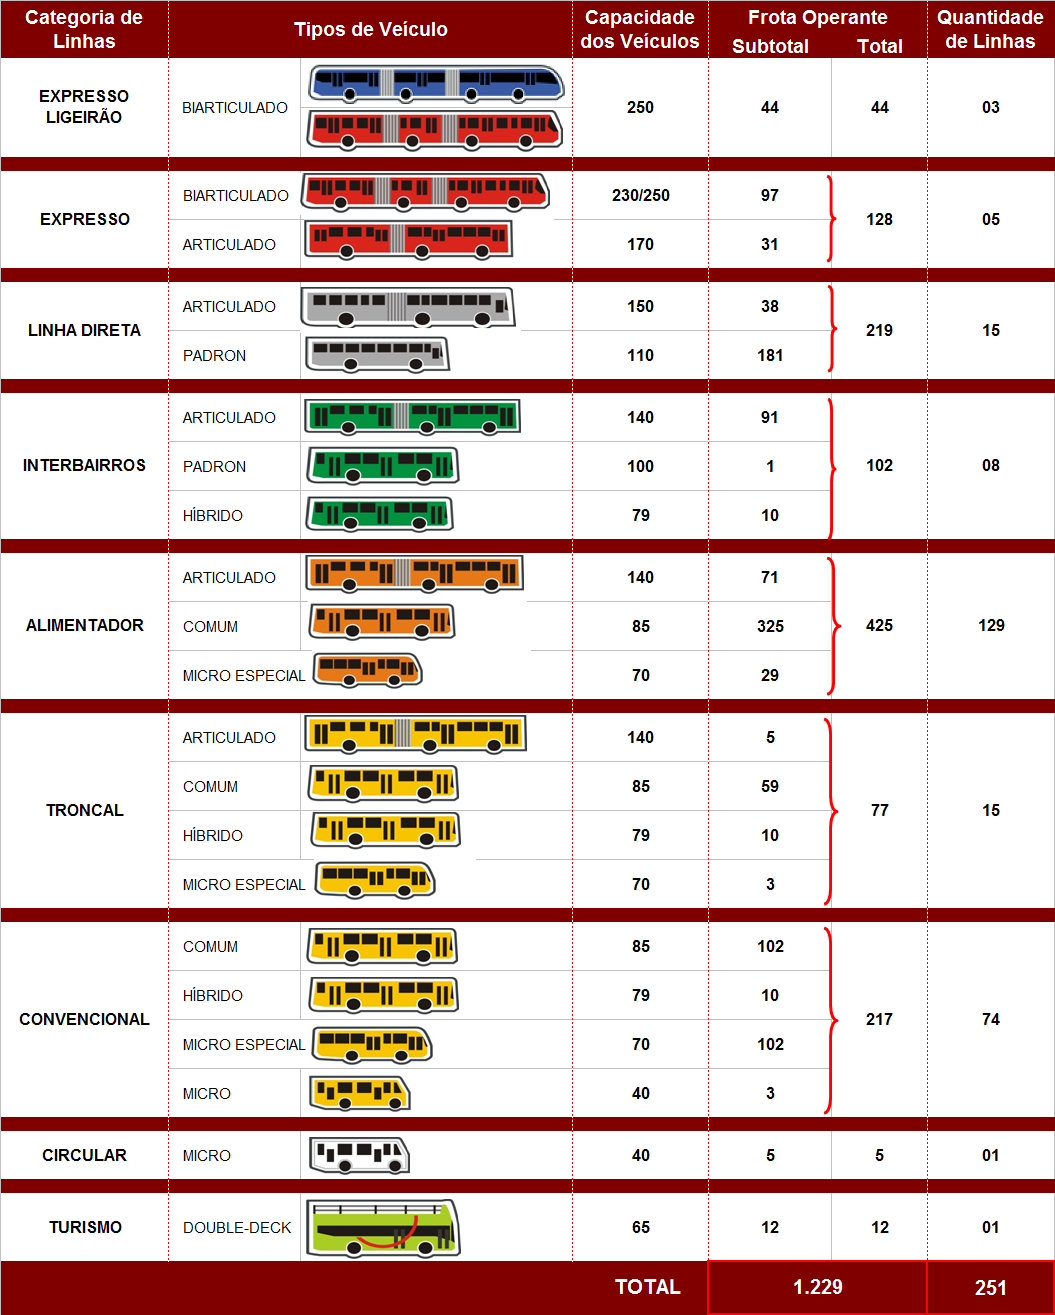
\includegraphics[scale=.40]{./Capitulo3/img/composicao-frota.png}
         \label{fig:linhas}
     \fonte{Rede Integrada de Transporte~\cite{Cur:19}}
 \end{figure}


Os terminais, assim como as linhas do transporte público são divididas em categorias e  recebem uma classificação sendo divididos em: terminais de ponta, terminais intermediários, terminais de bairros, terminais de área central e terminais metropolitanos. Tal divisão, como o nome sugere, indica a posição dos mesmos no sistema de transporte, conforme ilustra a Figura ~\ref{fig:terminais}.
 \begin{figure}[!h]
 \caption{Localização e classificação dos terminais de ônibus de Curitiba}
     \centering
     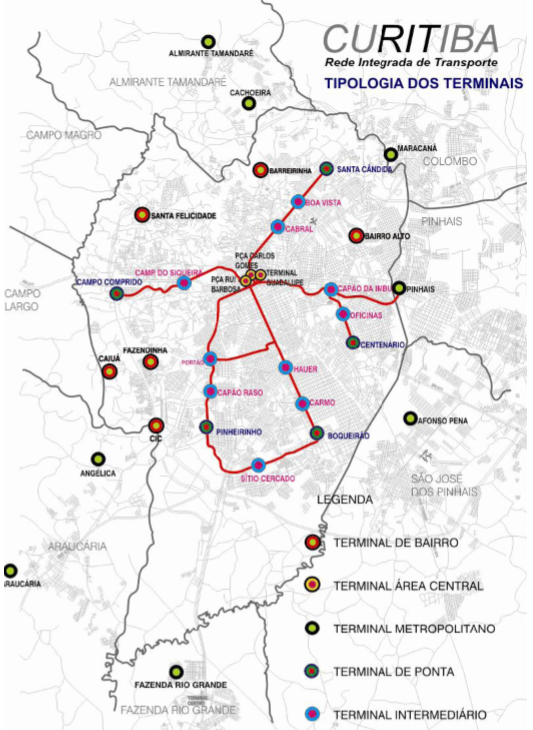
\includegraphics[scale=.95]{./Capitulo3/img/terminais.png}
         \label{fig:terminais}
     \fonte{Plano de Mobilidade Urbana de Curitiba, IPUCC 2019}
 \end{figure}

\section{Modelo Proposto} \label{sec:met}


O modelo proposto para o transporte público de Curitiba é mostrado na Figura~\ref{fig:model}. Este modelo tem por base o modelo de~\cite{wach:19}.

A Figura~\ref{fig:model} apresenta um grafo com vértices temporais (\emph{Line} e \emph{Trip} ) e espaço-temporais (\emph{BusStop} e \emph{Event}). Os vértices temporais carregam informações que variam com o tempo, enquanto os vértices espaço-temporais possuem informações de tempo associadas a dados de posicionamento georreferenciado. Vértices adicionais definem propriedades estáticas inerentes à operação de transporte público de Curitiba(\emph{Timetable}, \emph{ServiceCategory}, \emph{Color}, \emph{BusStopType} e \emph{Neighbourhood}), assim como agrupamentos temporais do modelo que permitem recuperar informações para diferentes escalas de tempo (\emph{Year}, \emph{Month}, \emph{Day} e \emph{Hour}). Em resumo, o modelo da Figura~\ref{fig:model} representa dependências temporais e espaço-temporais entre os vértices do grafo que descreve a operação de um sistema de transporte.

 \begin{figure}[!h]
 \caption{Modelo TVG da movimentação dos ônibus do transporte.}
     \centering
     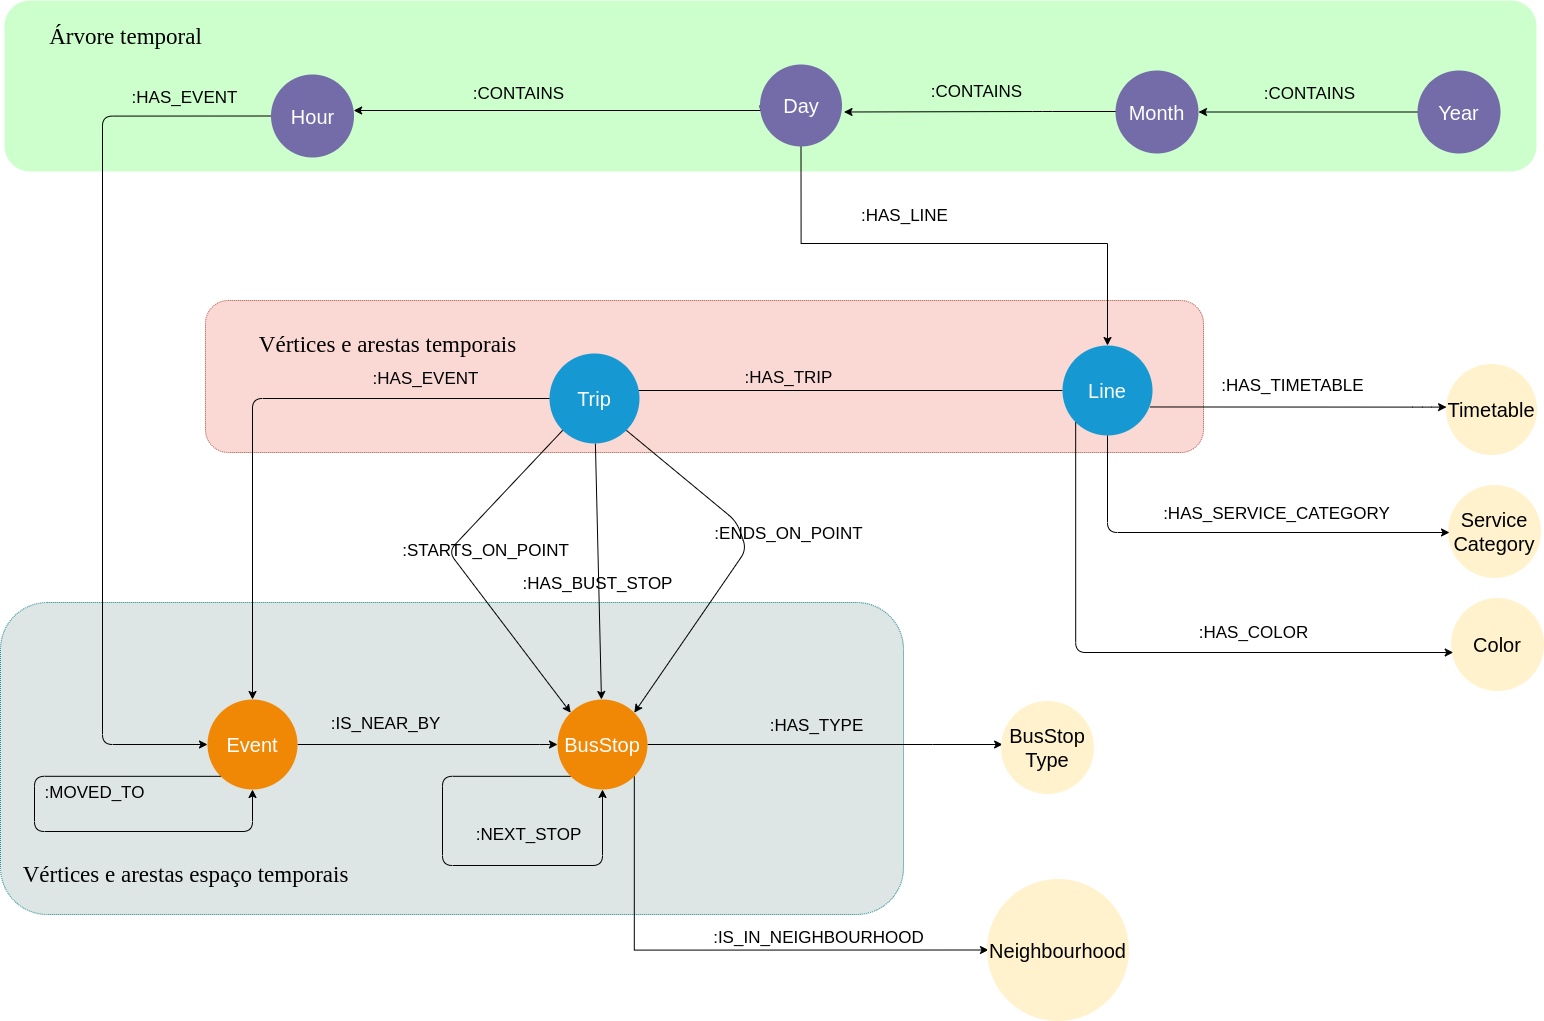
\includegraphics[scale=.25]{./Capitulo3/img/graph-model.png}
         \label{fig:model}
     \fonte{Autoria própria}
 \end{figure}
 
 

Os atributos dos vértices do grafo da Figura~\ref{fig:model} são mostrados nas Tabelas~\ref{tab:vertice_line}, \ref{tab:vertice_trip}, \ref{tab:vertice_busstop}, \ref{tab:vertice_event}, \ref{tab:vertice_color}, \ref{tab:vertice_service_category}, \ref{tab:vertice_busstop_type},\ref{tab:vertice_timetable} e \ref{tab:vertice_neighbourhood}. 

Cada linha de ônibus (vértices \emph{Line} - Tabela~\ref{tab:vertice_line}) dá origem a viagens (vértices \emph{Trip} - Tabela~\ref{tab:vertice_trip}).

As viagens são programadas (vértices \emph{Timetable} - Tabela~\ref{tab:vertice_timetable}) para serem executadas por veículos, que geram sequências de movimentação e paradas (vértices \emph{Event} - Tabela~\ref{tab:vertice_event}). Estas paradas incluem paradas nos pontos de ônibus (vértices \emph{BusStop} - Tabela~\ref{tab:vertice_busstop}) para embarque e desembarque de passageiros. Além disso, as viagens possuem pontos de ônibus inicial, intermédiario(s) e final (vértices \emph{BusStop} - Tabela~\ref{tab:vertice_busstop}). Além disso, linhas de ônibus podem ser agrupadas e recuperados por dia (aresta \texttt{HAS\_LINE}), assim como eventos podem ser agrupados e recuperados por hora (aresta \texttt{HAS\_EVENT}). Os atributos das arestas da Figura~\ref{fig:model} são mostrados na Tabela~\ref{tab:arestas} do Apêndice. As arestas estabelecem relacionamentos entre os vértices do grafo, além de carregarem atributos espaciais, temporais ou espaço-temporais para orientar consultas futuras.
Conforme será discutido na Seção~\ref{sec:impl}, a construção do grafo correspondente ao modelo da Figura~\ref{fig:model} no Neo4j é realizada a partir dos dados brutos da operação do transporte.


\subsection{Vértices}

Os vértices em roxo (\emph{year}, \emph{month}, \emph{day} e \emph{hour}) representam elementos essencialmente temporais representados. Tais elementos constituem a árvore temporal do grafo.

Já os vértices em azul representam elementos temporais relacionados ao modelo de transporte, sendo constituído pelos vértices \emph{Line} - Tabela~\ref{tab:vertice_line} e \emph{Trip} - Tabela ~\ref{tab:vertice_trip}:
 
\begin{table}[!htb]
    \caption{Atributos dos vértices \emph{Line}: identificam a linha de ônibus.}
    \label{tab:vertice_line}
    \centering
    \footnotesize
    \begin{tabular}{p{2.5cm}p{6cm}} 
    \hline
    Atributo & Descrição\\
    \hline
    \texttt{line\_name}        & nome da linha \\
    \texttt{card\_only}        & indicador se a linha aceita somente cartão \\
    \texttt{line\_code}        & código da linha \\
    \hline
    \end{tabular}
\end{table}


\begin{table}[htb]
    \caption{Atributos dos vértices \emph{Trip}: identificam os sentidos das linhas.}
    \label{tab:vertice_trip}
    \centering
    \footnotesize
    \begin{tabular}{p{2.5cm}p{2.5cm}}
        \hline
        Atributo & Descrição\\
        \hline
        \texttt{line\_way} & sentido da linha \\
        \hline  
    \end{tabular}
\end{table}


Vértices em laranja identificam elementos espaço-temporais na rede, isto é, que possuem atributos de geolocalização assim como relações temporais. No modelo são destacados os vértices \emph{BusStop} - Tabela ~\ref{tab:vertice_busstop} e \emph{Event} - Tabela~\ref{tab:vertice_event} :

\begin{table}[!htb]
    \caption{Atributos dos vértices \emph{BusStop}:  identificam os pontos de ônibus.}
    \label{tab:vertice_busstop}
    \centering
    \footnotesize
    \begin{tabular}{p{2.5cm}p{5cm}} 
        \hline
        Atributo & Descrição\\
        \hline
        \texttt{name} & nome do ponto de ônibus  \\
        \texttt{number} & número do ponto de ônibus \\
        \texttt{neighborhood\_code} & identificador único do bairro onde o ponto de ônibus está localizado\\
        \texttt{h3\_index10} & georreferenciamento h3 do ponto de ônibus  \\
        \texttt{latitude} & latitude do ponto \\
        \texttt{longitude} & longitude do ponto \\
        \hline
    \end{tabular}
\end{table}


\begin{table}[!htb]
    \caption{Atributos dos vértices \emph{Event}: identificam eventos de posicionamento dos ônibus.}
    \label{tab:vertice_event}
    \centering
    \footnotesize
    \begin{tabular}{p{3cm}p{6cm}} 
        \hline
        Atributo & Descrição\\
        \hline
        \texttt{moving\_status} & tipo do evento. [STOPPED, MOVING] \\
        \texttt{avg\_velocity} & velocidade do evento em km/h \\
        \texttt{event\_timestamp} & \emph{timestamp} do evento de parada do ônibus  \\
        \texttt{latitude} & latitude da parada  \\
        \texttt{longitude} & longitude da parada  \\
        \texttt{vehicle} & identificador único do veículo \\
        \hline  
    \end{tabular}
\end{table}

Vértices em amarelo identificam definem propriedades estáticas inerentes à operação de transporte público de Curitiba. Estes são constituídos pelos vértices \emph{Timetable} - Tabela~\ref{tab:vertice_timetable}, \emph{ServiceCategory} - Tabela~\ref{tab:vertice_service_category}, \emph{Color}- Tabela~\ref{tab:vertice_color}, \emph{BusStopType}- Tabela~\ref{tab:vertice_busstop_type} e \emph{Neighbourhood})- Tabela~\ref{tab:vertice_neighbourhood}.
 

\begin{table}[htb]
    \caption{Atributos dos vértices \emph{Timetable}: identificam os horários programados das linhas.}
    \label{tab:vertice_timetable}
    \centering
    \footnotesize
    \begin{tabular}{p{2.5cm}p{6.5cm}}
        \hline
        Atributo & Descrição\\
        \hline
        \texttt{start\_time} & horário programado para o inicio da viagem \\
        \texttt{end\_time} & horário programado para o término da viagem \\
        \texttt{line\_way} & sentido da viagem \\
        \texttt{start\_point} & ponto de ônibus onde a viagem se inicia \\
        \texttt{end\_point} & ponto de ônibus onde a viagem termina \\
        \texttt{timetable} & número da tabela de agendamento de horários \\
        \hline  
    \end{tabular}
\end{table}

\begin{table}[htb]
    \caption{Atributos dos vértices \emph{ServiceCategory}: identificam as categorias de serviço das linhas.}
    \label{tab:vertice_service_category}
    \centering
    \footnotesize
    \begin{tabular}{p{2.5cm}p{6.5cm}}
        \hline
        Atributo & Descrição\\
        \hline
        \texttt{value} & nome da categoria de serviço da linha \\
        \hline  
    \end{tabular}
\end{table}

\begin{table}[htb]
    \caption{Atributos dos vértices \emph{Color}: identificam as cores das linhas.}
    \label{tab:vertice_color}
    \centering
    \footnotesize
    \begin{tabular}{p{2.5cm}p{6.5cm}}
        \hline
        Atributo & Descrição\\
        \hline
        \texttt{value} & nome da cor \\
        \hline  
    \end{tabular}
\end{table}

\begin{table}[htb]
    \caption{Atributos dos vértices \emph{BusStopType}: identificam as tipos de pontos de ônibus.}
    \label{tab:vertice_busstop_type}
    \centering
    \footnotesize
    \begin{tabular}{p{2.5cm}p{6.5cm}}
        \hline
        Atributo & Descrição\\
        \hline
        \texttt{value} & nome do tipo de ponto de ônibus \\
        \hline  
    \end{tabular}
\end{table}

\begin{table}[htb]
    \caption{Atributos dos vértices \emph{Neighbourhood}: identificam os bairros da cidade de Curitiba.}
    \label{tab:vertice_neighbourhood}
    \centering
    \footnotesize
    \begin{tabular}{p{2.5cm}p{2.5cm}}
        \hline
        Atributo & Descrição\\
        \hline
        \texttt{name} & nome do bairro \\
        \texttt{code} & identificador único do bairro \\
        \texttt{section\_name} & nome da regional \\
        \texttt{section\_code} & código da regional \\
        \texttt{h3\_index10} & georreferenciamento h3 do bairro \\
        \hline  
    \end{tabular}
\end{table}


\subsection{Arestas}

As arestas conectam dois vértices de um grafo. Elas e seus atributos são descritos na Tabela~\ref{tab:arestas}.

\begin{table}[!htb]
    \caption{Descrição das arestas: significado das conexões e atributos.}
    \label{tab:arestas}
    \centering
    \small
    \begin{tabular}{ p{5cm}p{8.5cm}} 
    \hline
    Rótulo & Descrição\\
    \hline
    \texttt{IS\_NEAR\_BY}            & conecta o ônibus a paradas (veloc. $< 15$ km/h)\\
    \texttt{STARTS\_ON\_POINT}       & Conecta um sentido de linha a seu ponto de ônibus inicial determinando o início de seu roteiro. \\
    \texttt{HAS\_BUST\_STOP}         & Identifica os pontos de ônibus que compõe um sentido da linha\\
    \texttt{ENDS\_ON\_POINT}         & Conecta um sentido de linha a seu ponto de ônibus final determinando o término de seu roteiro. \\
    \texttt{HAS\_COLOR}              & conecta a linha a sua cor \\ 
    \texttt{HAS\_TYPE}               & conecta o ponto de ônibus ao seu tipo \\ 
    \texttt{HAS\_SERVICE\_CATEGORY}  & conecta a linha a sua categoria de serviço \\ 
    \texttt{IS\_IN\_NEIGHBOURHOOD}   & conecta o ponto de ônibus ao bairro em que está localizado \\ 
    \texttt{HAS\_TIMETABLE}          & conecta a linha à sua programação horária \\ 
    \texttt{HAS\_TRIP}               &  Uma linha pode ter diversos sentidos: logo, esta aresta realiza a conexão da linha com os sentidos da linha. \\ 
    \texttt{HAS\_LINE}               & Conecta a árvore temporal a existência da linha operante. Uma linha pode deixar de operar ao longo do tempo. \\ 
    \texttt{HAS\_EVENT}              & agrupa as informações de eventos do veículo por hora\\
    \hline
    \multirow{4}{*}{\texttt{NEXT\_STOP}} & conecta pontos de ônibus consecutivos da viagem: \\
    & \texttt{line\_code}: Código da linha\\
    & \texttt{line\_way}: Sentido da linha\\
    & \texttt{distance}: Distância em metros entre dois pontos de ônibus \\
    & \texttt{line\_name}: Nome da linha\\
    \hline
    \multirow{4}{*}{\texttt{MOVED\_TO}}           & Liga a sequência de eventos de um determinado veículo. \\
    & \texttt{delta\_time\_in\_sec}: Tempo em segundos entre dois eventos.\\
    \hline
    \end{tabular}
\end{table}



\section{Métricas de Redes Complexas} \label{sec:metr}


Uma vez que o grafo do sistema de transporte descrito na seção anterior é modelado e armazenado no Neo4j, métricas de redes complexas podem ser computadas para avaliar o comportamento do sistema. 
Tais métricas permitem uma avaliação da importância dos vértices na rede (pontos de ônibus), tanto do ponto de vista estático da topologia da rede quanto dinâmico da movimentação dos ônibus, e sua relação com os outros pontos da rede.
Esta seção descreve as métricas utilizadas neste trabalho: 

\subsection{Centralidade de grau}


Proposto por~\cite{free:79}, a {\bf centralidade de grau} é proporcional ao número de arestas (de entrada, ou de saída em grafos direcionados) que se conectam a um determinado vértice. Quanto maior a centralidade de grau de um vértice, maior é o número de conexões com outros vértices.

No caso da rede de transporte, na perspectiva de dinamicidade da rede através da interatividade de veículos com seus respectivos pontos de ônibus, a centralidade de grau de um vértice \emph{BusStop} é proporcional ao número de paradas de ônibus no respectivo ponto. Isso pode significar que pontos com elevada centralidade de grau podem corresponder a locais de potencial congestionamento ou de formação de comboios decorrente de uma estratégia de atendimento de demanda elevada. 

Na perspectiva da rede estática, isto é, isolando-se somente os pontos de ônibus e suas conexões, a centralidade de grau de um vértice \emph{BusStop} é proporcional ao número de linhas de ônibus que passam pelo vértice, já que apenas arestas para outros vértices \emph{BusStop} são consideradas. Um ponto ponto de ônibus com grande número de conexões apresenta uma grande oferta de linhas.

\subsection{Centralidade de intermediação}


Introduzido por \cite{free:77} como uma medida para quantificar o controle de um ser humano sobre a comunicação entre outros seres humanos em uma rede social, a {\bf centralidade de intermediação} (\emph{betweenness centrality}) quantifica quão importante um vértice (ou uma aresta) é na definição dos caminhos possíveis entre vários (ou todos) os pares de vértices de uma rede. Isso permite calcular qual a capacidade da rede se ``recuperar'' em caso de remoção de um ou mais vértices. Também é importante, pois auxilia na identificação de vértices que atuam como ``intermediários de serviços'' na rede.

Em outras palavras, a remoção de vértices com elevada centralidade de intermediação podem degradar ou mesmo interromper o fluxo de informação em uma rede. 

Para um vértice, a centralidade de intermediação é definida pela proporção dos caminhos que empregam um determinado vértice em relação a todos os caminhos existentes, ou seja:

 \begin{equation}
     B(u) = \sum_{s \neq u \neq t }^{} p(u) / p,
 \end{equation} 
na qual:

 \begin{itemize}
 \item $u$: é um vértice.
 \item $p$: é o número total de caminhos entre os vértices $s$ e $t$.
 \item $p(u)$: é o número de caminhos entre os vértices $s$ e $t$ que passam pelo vértice $u$.
\end{itemize}  

No contexto de sistemas de transporte, vértices com significativo $B$ são potenciais pontos de estrangulamento do sistema, dada a dependência que os caminhos possíveis desse sistema têm desse vértice. Essa dependência pode ser temporal (ocorre em um intervalo de tempo específico) ou espacial (depende da posição espacial do ponto de ônibus), de acordo com o contexto de análise.

\subsection{Page rank}


O {\bf \emph{page rank}} foi concebido com o intuito de ranquear páginas (\emph{web sites}) relevantes da \emph{World Wide Web}. 

Usando o conceito presente em cadeias de Markov e/ou difusão em redes complexas, pode-se determinar os vértices mais significativos do ponto de vista de fluxos existentes em uma rede, quando o regime estacionário é atingido. Pode-se traduzir esse regime estacionário como a tendência de um usuário aleatório sempre chegar em uma determinada página, ou os dados em redes de comunicação sempre trafegarem por um determinado roteador.

A ideia é que o fluxo de navegação dos usuários defina a relevância das páginas ao reforçar suas interconexões (\emph{hyperlinks}). O algoritmo PageRank \cite{brin:98} traduz a ideia intuitiva de que usuários em geral tendem a acessar páginas e navegar pela WWW usando \emph{hiperlinks} até uma certa profundidade. Assim, páginas bem posicionadas no fluxo de navegação são relevantes, pois tendem a ser muito visitadas pelos usuários. 
No contexto das redes de transporte, um ponto de ônibus com elevado \emph{page rank} pode indicar conexões com outros pontos importantes. Por exemplo, ligações diretas entre terminais de ônibus no caso estático.


\subsection{Caminho mínimo}

O {\bf caminho mínimo} entre dois vértices é o caminho com o menor número de arestas, no caso de arestas não ponderadas. 
Define-se caminho entre dois vértices quaisquer como a sequência de vértices, ligados dois a dois por arestas, que deve ser percorrida para conectá-los. As arestas podem ser ponderadas ou não, definindo características das ligações entre dois vértice e afetando a definição do caminho. A partir dos caminhos existentes entre dois nós quaisquer, define-se como caminho mais curto aquele cujo ``esforço'' exigido para percorrê-lo é o menor dentre os caminhos existentes.

Caso as arestas sejam ponderadas, deve-se considerar a soma dos pesos das arestas do caminho de um vértice a outro. A determinação de caminhos mínimos (considerando todos os pares de vértices de uma rede) é informação significativa para o planejamento urbano e a operação de um sistema de transporte, pois pode induzir no fluxo de pessoas na cidade. Algoritmos de caminho mínimo identificam rotas de conexão entre dois pontos da cidade de forma a minimizar o tempo de percurso necessário no transporte público \cite{Mart:2009, Larson:81}. Uma vez conhecidos os caminhos mínimos de todos os vértices para todos os outros da rede, define-se o {\bf diâmetro da rede} como o caminho mínimo mais longo da rede.

% \subsection{Conectividade}

% \textcolor{courb2020}{
% Conectividade é um propriedade que indica existe pelo menos um caminho entre todos os pares de vértices de uma rede. Caso não haja, existem sub-grafos isolados dentro da rede.
% No contexto das redes TVGs aplicadas ao sistema de transporte público, a evolução temporal desse sistema pode ou não gerar intervalos de tempo nos quais parte da rede perde conectividade com o restante da rede. Essa mudança na conectividade da rede pode ser um comportamento estrutural (ou seja, é um fenômeno recorrente da rede) ou uma anomalia (um fenômeno aleatório, como um acidente que bloqueie a passagem de veículos por uma via pública).
% }

\subsection{Diâmetro e densidade de rede}

A partir do resultado do cálculo de caminhos e caminhos mínimos pode ser identificado o diâmetro (geodésico) de uma rede. O diâmetro de uma rede é o caminho mínimo mais longo dessa rede, ou seja, a distância entre dois vértices cujo caminho mínimo é o mais longo a ser percorrido. 

Naturalmente, o contexto de análise pode implicar que o diâmetro possa ser calculado a partir de atributos dos vértices e/ou arestas, como tempo exigido para percorrer dada par de vértice conectado, ou a distância entre esses pares de vértices conectados.
A densidade da rede mede a similaridade entre a rede e um grafo completo (grafo em que há um aresta para todos os seus pares de vértices) e pode ser definida como:

 \begin{equation}
     D = \mid E \mid / \mid N \mid ( \mid N \mid -1),
 \end{equation} 
na qual:

 \begin{itemize}
 \item $N$: é o número total de vértices.
 \item $E$: é o número total de arestas.
\end{itemize}  


\section{Plataforma Computacional} \label{sec:impl}

A plataforma computacional desenvolvida gera um banco de dados de grafo no Neo4j a partir do \emph{dataset} disponibilizado pela operação do transporte coletivo de Curitiba.


\subsection{Dataset}

\textcolor{courb2020}{
O portal de dados abertos de Curitiba fornece diariamente um \emph{dataset} em formato JSON (JavaScript Object Notation) com informações sobre o transporte coletivo da cidade. Conforme mencionado anteriormente, o transporte opera em média com uma frota de 1.410 ônibus que atende cerca de 1.389.731 passageiros por dia com 251 linhas de ônibus, 329 estações e 21 terminais.
}

\textcolor{courb2020}{
A empresa URBS (gestora da Rede Integrada de Transporte Coletivo de Curitiba) define um conjunto de tabelas que contêm informações referentes às linhas de ônibus existentes, seus pontos de parada (que podem atender múltiplas linhas), os itinerários das linhas, os veículos que percorrem essas linhas, o percurso georeferenciado das linhas e o relacionamento entre essas informações. A descrição destas tabelas pode ser encontrada no dicionário de dados disponível no repositório de dados abertos. 
}
%\peix{Tais informações também estão disponíveis em forma de web service e pode ser acessado mediante a solicitação de login e senha. O dicionário de dados contendo a descrição das informações disponibilizadas pode ser obtido em \cite{dadosabertos}}

\textcolor{courb2020}{
Parte destes dados, que alimentam o fluxo de transformações descrito na Seção~\ref{subsec:work}, são detalhados nas Tabelas~\ref{tab:linhas}, \ref{tab:pontos_linha}, \ref{tab:tabela_veiculo} e \ref{tab:veiculos} do Apêndice.
}

%\ric{Seria importante caracterizar também a dimensão desta base. Por exemplo, para 1 mês de captura de dados, estamos falando de qual volume de dados? Mostrar em uma tabela: número de linhas, viagens, ônibus, etc?}


% \ric{A Tabela~\ref{tab:data} mostra estatísticas do \emph{dataset} utilizado, com informações sobre o transporte coletivo de Curitiba coletados durante um mês de operação.}

% \begin{table}[h]
%     \caption{Estatísticas do \emph{dataset} do transporte de Curitiba para 1 mês de operação \mar{(qual mês/ano?)}.}
%     \label{tab:data}
%     \centering
%     \begin{tabular}{ccccc} 
%         \hline
%         No. de registros? &No. de linhas &No. de pontos &No. de ônibus &No. de viagens\\
%         \hline
%         xxx &xxx &xxx &xxx &xxx \\
%         \hline  
%     \end{tabular}
% \end{table}

%\ric{É IMPORTANTE? É importante salientar que essas tabelas apresentam redundâncias de dados, pois não foram normalizadas segundo preceitos de banco de dados. Isso significa que foi necessário pré-processá-lo para identificar e remover inconsistências.}

\subsection{Python}


Criada na década de 1980 por Guido van Rossum na Holanda, Python é uma linguagem de programação multifuncional de alto nível que é usada em um ampla gama de domínios e campos técnicos~\cite{Yves:2018}.

Python é uma linguagem de programação interpretada, orientada a objetos e de alto nível, com tipagem dinâmica, o que o torna muito atraente para o desenvolvimento rápido de aplicativos, assim como para uso como uma linguagem de \emph{script} com a finalidade de conectar componentes existentes.
Sua sintaxe é simples e de fácil aprendizado enfatizando a legibilidade e manutenibilidade de código. Python suporta módulos e pacotes, incentivando assim a modularização de programas e reutilização de código.
 
Atualmente, a linguagem Python é amplamente utilizada, desde universidades nas mais diversas áreas científicas, até grandes corporações e instituições financeiras.

Segue algumas das principais características da linguagem Python:

\begin{itemize}

\item \emph{Open source}: Python e a maioria das bibliotecas e ferramentas de suporte disponíveis são
open source e geralmente vêm com licenças bastante flexíveis e abertas.

\item Interpretada: Python utiliza um interpretador denominado CPyhon que traduz o código fonte em tempo de execução para código \emph{byte code} executável.

\item Multi paradigma: Python suporta diferentes paradigmas de programação como orientação a objetos, funcional ou programação procedimental.

\item Multi propósito: Python pode ser utilizado para desenvolvimento de código rápido e interativo, bem como para construir grandes aplicações.

\item \emph{Cross-platform}: Python está disponível nos mais conhecidos sistemas operacionais, tais como, \emph{Windows}, \emph{Linux} e \emph{MacOS} e pode ser utilizado para o desenvolvimento de aplicações \emph{Desktop}, assim como aplicações \emph{Web}. Além disso Python pode ser utilizado em grandes conjuntos de \emph{clusters} e servidores potentes, assim como em pequenos dispositivos como \emph{Raspberry Pi}.

\item Dinamicamente tipada: Tipos de dados em Python são inferidos em tempo de execução e não previamente declarados como na maioria das linguagens de programação compiladas. 

\item Indentação ciente: Em contraste com a maioria das outras linguagens de programação, Python usa indentação para marcar blocos de código em vez de parênteses, colchetes ou ponto e vírgula.

\item \emph{Garbage collector}: Python possui \emph{garbage collection} automatizado, o que evita a necessidade do gerenciamento de memória pelo programador.

\end{itemize}


\subsection{Neo4J}

Neo4J (\emph{Network Exploration and Optimization 4 Java}) é um sistema gerenciador de banco de dados não relacional, orientado à grafos, desenvolvido pela empresa Neo Technology. É implementado em Java e acessível por programas escritos em outras linguagens utilizando \emph{Cypher Query Language} através de um \emph{endpoint} HTTP ou através de um protocolo denominado \emph{bolt}.
Neo4J é open-source em sua versão "community edition" e está disponível através de uma licença  GPLv3 (General Public License) para a versão Community Edition, e AGPLv3 (Affero General Public License) para versão Enterprise Edition.

O banco de dados Neo4j implementa um tipo de grafo denominado \emph{property graph model}, capaz de representar multigrafos direcionados, rotulados e com atributos. Estes grafos permitem a representação de vértices e arestas rotulados, além de metadados (propriedades) associados aos vértices e arestas~\cite{rod:10}, particularmente importantes na implementação de TVGs. Além disso, o banco de dados Neo4j tem outras características que favorecem a implementação: (i) armazenamento persistente e transacional de grafos de elevada dimensão; suporte para análise em profundidade via buscas eficientes de múltiplos saltos; (iii) suporte para linguagem declarativa de \emph{queries} de grafos denominada Cypher\footnote{https://neo4j.com/docs/cypher-manual/current/}.


This graph data model gives us four different fundamental building blocks to
structure and store our data. Let's go through them:


 \begin{figure}[!h]
 \caption{Property Graph Model}
     \centering
     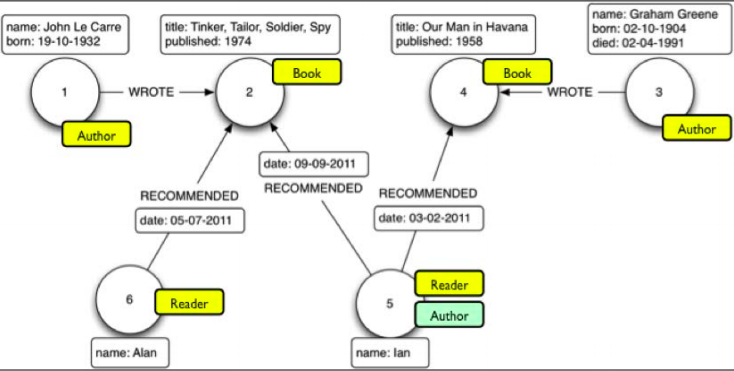
\includegraphics[scale=.60]{./Capitulo3/img/grafo-rotulado.png}
         \label{fig:propertygraphmodel}
     \fonte{Property Graph Model~\cite{bruggen:2014}}
 \end{figure}
 

•   Nodes: These are typically used to store entity information. In the preceding
example, these are the individual books, readers, and authors that are present
in the library data model.

•	 Relationships: These are used to connect nodes to one another explicitly
and therefore provide a means of structuring your entities. They are the
equivalent of an explicitly stored, and therefore pre-calculated, join-like
operation in a relational database management system. As we have seen
in the previous chapters, joins are no longer a query-time operation—they
are as simple as the traversal of a relationship connecting two nodes.
Relationships always have a type, a start- and an end-node, and a direction.
They can be self-referencing/looping and can never be dangling (missing
start- or end-node).

•	 Properties: Both nodes and relationships are containers for properties,
which are effectively name/value pairs. In the case of the nodes, this is
very intuitive. Just like a record in the relational database world has one or
more fields or attributes, so can the node have one or more properties. Less
intuitive is the fact that relationships can have properties too. These are used
to further qualify the strength or quality of a relationship and can be used
during queries/traversals to evaluate the patterns that we are looking for.

 Labels: This was a fundamental data model construct that was added to
Neo4j with Version 2.0 at the end of 2013. Labels are a means to quickly and
efficiently create subgraphs. By assigning labels to nodes, Neo4j makes the
data model of most users a lot simpler. There is no longer a need to work
with a type property on the nodes, or a need to connect nodes to definition
nodes that provide meta-information about the graph. Neo4j now does
this out of the box—and this is a huge asset, now and for the future. At
the time of writing this book, labels are primarily used for indexing and
some limited schema constraints. However, in future, it is likely that the
structural understanding that labels provide about the data stored in the
graph will be used for other purposes such as additional schema, security,
graph sharding/distribution—and perhaps others.


Uma das importantes funcionalidades do Neo4J é a utilização de plugins e bibliotecas para consulta ao banco de dados e execução de algoritmos de redes complexas. 
Dentre as várias bibliotecas podemos citar a \emph{Neo4j Graph Algorithms} que fornece um conjunto de procedimentos definidos pelo usuário que podem ser executadas através da linguagem de consulta Cypher.  
A biblioteca \emph{Neo4j Graph Algorithms} inclui algoritmos para análise de grafos e fluxos de trabalho de aprendizado de máquina com suporte a até dezenas de bilhões de nós e relacionamentos.

Outra biblioteca muito importante utilizada neste trabalho é a \emph{Neo4j Awesome Procedures on
Cypher (APOC)}. Esta biblioteca consiste em mais de 450 procedimentos e funções que auxiliam tarefas comuns como integração de dados, conversão de tipagem de dados e refatoração de modelos.


CYPHER

One of the defining features of the Neo4j graph database product today is its
wonderful query language, called Cypher. Cypher is a declarative, pattern-matching
query language that makes graph database management systems understandable and
workable for any database user—even the less technical ones.
The key characteristic of Cypher is, in my opinion, that it is a declarative language,
opposed to other imperative query languages that have existed for quite some time.

Why is this so important? Here are your answers:

•	 Declarative languages allow you to state what you're looking for, declare
the pattern that you would like to see retrieved, and then let the database
worry about how to go about retrieving that data.
In an imperative (query) language, you would have to tell the database
specifically what to do to get to the data and retrieve i


Declarative languages separate the concern of stating the problem, from
solving it. This allows greater readability of the queries that you write,
which is important as people tend to read their database queries more
often than they write them. This piece of your software will therefore
become more readable and shareable with others, and long term
maintenance of that easy-to-read query becomes so much easier.

•	 Declarative languages will allow the database to use the information that
it holds about the nature and structure of the data to answer your question
more efficiently. Essentially, it allows query optimizations that you would
never have known of or thought about in an imperative approach. Therefore,
declarative languages can be faster—at least over time as the optimization
algorithms mature.

•	 Declarative languages are great for adhoc querying of your database,
without you having to write complex software routines to do so.

\subsection{Apache Spark}


Apache Spark (doravante apenas Spark) é um mecanismo de análise para dados em grande escala pro‐
cessação. Ele usa uma abstração de tabela chamada DataFrame para representar e processar dados em
linhas de colunas nomeadas e digitadas. A plataforma integra diversas fontes de dados e
suporta linguagens como Scala, Python e R. Spark oferece suporte a várias análises
bibliotecas. Seu sistema baseado em memória opera usando gráficos de computação distribuídos de forma eficiente.

Apache Spark (henceforth just Spark) is an analytics engine for large-scale data pro‐
cessing. It uses a table abstraction called a DataFrame to represent and process data in
rows of named and typed columns. The platform integrates diverse data sources and
supports languages such as Scala, Python, and R. Spark supports various analytics
libraries, as shown in Figure 3-1. Its memory-based system operates by using efficiently distributed compute graphs.


\subsection{Transformação do \emph{dataset} para a base de dados de grafo do Neo4j}
\label{subsec:work}

A Figura~\ref{fig:workflow} mostra o fluxo de transformação dos dados para a construção do modelo de grafo no Neo4j a partir do \emph{dataset} disponibilizado. Diversos fluxos foram implementados na linguagem Python usando a ferramenta Apache Spark\footnote{https://spark.apache.org/}. 


 \begin{figure}[!h]
 \caption{Fluxo de ingestão de dados}
     \centering
     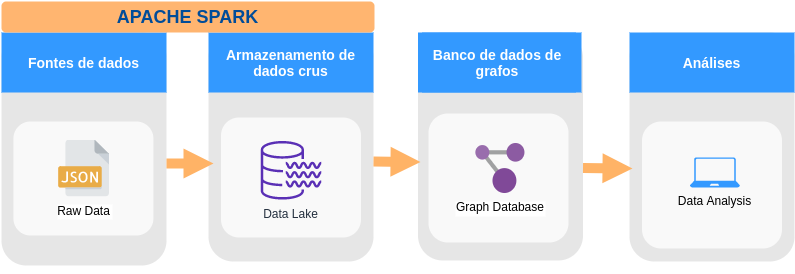
\includegraphics[scale=.45]{./Capitulo3/img/data-flow.png}
         \label{fig:dataflow}
     \fonte{Autoria própria}
 \end{figure}
 
 
A primeira etapa consiste no carregamento dos dados brutos (em formato JSON) para uma área temporária de armazenamento (ou \emph{data lake}). Os arquivos JSON são transformados em arquivos parquet\footnote{https://parquet.apache.org/} \cite{Boufea:17} utilizando o Apache Spark. Arquivos parquet são formatos de armazenamento em colunas, otimizados para compressão e rápida recuperação de dados. 
%Nesta etapa é realizada somente a transformação de formato de arquivo e armazenamento de dados em uma área denominada data lake.
Na sequência, o conteúdo do \emph{data lake} é processado - também usando o Apache Spark - para gerar arquivos no formato CSV com os vértices e arestas do modelo de grafo apresentado na Seção~\ref{sec:met}. 

Embora vários fluxos de transformação de dados tenham sido implementados, detalha-se a seguir as transformações dos dados que criam o vértice \emph{Stop} e a aresta \texttt{EVENT\_STOP} do grafo. Estas estruturas modelam a dinâmica de movimentação dos ônibus e justificam o uso de um grafo variante no tempo.
%\mar{(Keiko e Ricardo: mexi nessa linha. Veja se melhorou.}

% O vértice \emph{Stop} é criado a partir da tabela \emph{VEICULOS} (Tabela~\ref{tab:veiculos} do Apêndice), que contém a geolocalização dos ônibus nos respectivos instantes de tempo. Com essa informação, calcula-se a distância percorrida, o tempo decorrido entre posicionamentos consecutivos e a velocidade média em km/h. Se a velocidade for menor do que 15 km/h, assume-se que houve uma parada do ônibus neste intervalo de tempo e um vértice \emph{Stop} é gerado no grafo com os respectivos atributos.

O vértice \emph{Stop} é criado a partir dos dados de geolocalização dos ônibus nos respectivos instantes de tempo (ver descrição da tabela \emph{VEICULOS} no dicionário de dados do repositório). Com essa informação, calcula-se a distância percorrida, o tempo decorrido entre posicionamentos consecutivos e a velocidade média em km/h. Se a velocidade for menor do que 15 km/h, assume-se que houve uma parada do ônibus neste intervalo de tempo e um vértice \emph{Stop} é gerado no grafo com os respectivos atributos.

% A aresta \texttt{EVENT\_STOP} é criada a partir dos vértices \emph{Stop} previamente obtidos das linhas dos ônibus, dos pontos de ônibus e da tabela horária dos ônibus nas linhas (Tabelas~\ref{tab:linhas}, \ref{tab:pontos_linha} e \ref{tab:tabela_veiculo} do Apêndice, respectivamente). Se uma parada (vértice \emph{Stop}) ocorrer a menos de 20 m de um ponto de ônibus (vértice \emph{Bus Stop}), considera-se que tal parada ocorreu em um ponto de ônibus e, portanto, cria-se uma aresta \texttt{EVENT\_STOP} para conectar os vértices \emph{Stop} e \emph{Bus Stop} no grafo.
% Uma vez construído o banco de dados de grafo para o transporte, consultas e análises de redes complexas podem ser realizadas a partir do Neo4j (\emph{Data Analysis} na Figura~\ref{fig:workflow}).

A aresta \texttt{EVENT\_STOP} é criada a partir dos vértices \emph{Stop} previamente obtidos das linhas dos ônibus, dos pontos de ônibus e da tabela horária dos ônibus nas linhas (ver descrição das tabelas \emph{LINHAS}, \emph{PONTOS\_LINHA} e \emph{TABELA\_VEICULO}, respectivamente, no dicionário de dados do repositório). Se uma parada (vértice \emph{Stop}) ocorrer a menos de 20 m de um ponto de ônibus (vértice \emph{Bus Stop}), considera-se que tal parada ocorreu em um ponto de ônibus e, portanto, cria-se uma aresta \texttt{EVENT\_STOP} para conectar os vértices \emph{Stop} e \emph{Bus Stop} no grafo.
Uma vez construído o banco de dados de grafo para o transporte, consultas e análises de redes complexas podem ser realizadas a partir do Neo4j (\emph{Data Analysis} na Figura~\ref{fig:workflow}).
 
%% Comente para remover este item

%% Capítulo
%%%% CAPÍTULO 4 - RESULTADOS E DISCUSSÃO
%%
%% Deve descrever detalhadamente os dados obtidos 
%% pelo autor. Normalmente são incluídas ilustrações
%% como: quadros, tabelas, gráficos, etc. Deve efetuar
%% a comparação dos dados obtidos e/ou resultados, com
%% aqueles descritos na revisão de literatura, 
%% incluindo os comentários sobre os estudos de outros
%% autores.

%% Título e rótulo de capítulo (rótulos não devem conter caracteres especiais, acentuados ou cedilha)
\chapter{Resultados e Discussão}\label{cap:resultadosediscussao}

% Deve descrever detalhadamente os dados obtidos pelo autor. Normalmente são incluídas ilustrações como: quadros, tabelas, gráficos, etc. Deve efetuar a comparação dos dados obtidos e/ou resultados, com aqueles descritos na revisão de literatura, incluindo os comentários sobre os estudos de outros autores.

\ric{Vamos organizar o capítulo da seguinte forma:}

\begin{enumerate}
    \item Análise exploratória: resultados estatísticos (visualizações) que permitam caracterizar de forma geral a base de dados utilizada;
    \item Operação da rede de transporte: resultados obtidos do uso de grafos temporais na caracterização da operação atual da rede de transporte de Curitiba;
    \item Integração temporal: resultados do estudo de uma integração temporal na rede de transporte de Curitiba
\end{enumerate}

\section{Análise exploratória}

Os resultados foram obtidos para o período de  01/03/2019 a 30/06/2019, tendo sido coletados 33 Gigabytes de dados, com 293.390.175 registros de geolocalização dos 1708 ônibus em operação. Este volume de dados gerou, após a transformação para o banco de dados de grafo do Neo4j, 26.869.679 vértices e 93.082.943 arestas.

%\ric{Seria importante apresentar uma tabela com um resumo das principais características dos dados utilizados (data de coleta dos dados, no. de linhas, pontos, etc.) e do banco obtido (no. de nós - linhas, trips, stops, bus stops, etc.), no. de arestas em geral, etc. Além disso, o tempo de computação necessário para gerar o banco no Neo4j.}

A Tabela~\ref{tab:neo} mostra estatísticas do banco de dados construído no Neo4j, com informações sobre o transporte coletivo de Curitiba coletados durante o período de 01/03/2019 a 30/06/2019.

\begin{table}[h]
    \caption{Estatísticas do banco de dados de grafo construído.}
    \label{tab:neo}
    \centering
    \begin{tabular}{ccc} 
        \hline
        No. vértices & No. de arestas & ???\\
        \hline
        26.869.679 & 93.082.943 & xxx \\
        \hline  
    \end{tabular}
\end{table}



\section{Operação da rede de transporte}

\ric{Resultados que podem ser derivados da modelagem proposta usando grafos temporais. Mais ou menos na linha do artigo do Courb.}

\begin{figure}
\centering
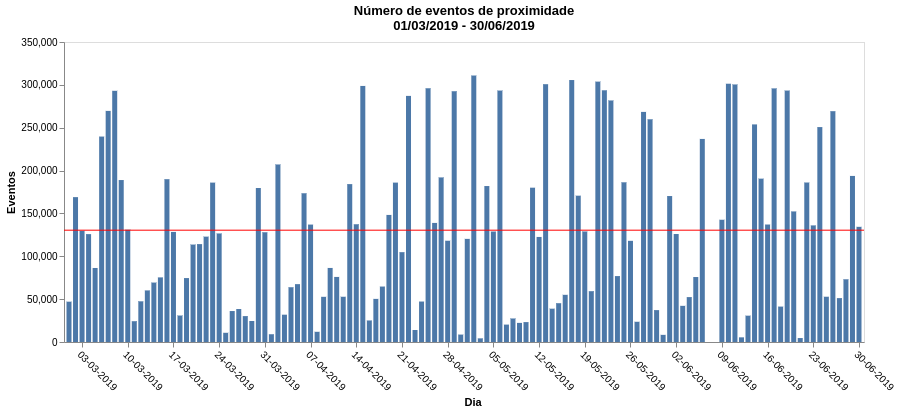
\includegraphics[width=.9\textwidth]{Capitulo4/img/eventos_proximidade.png}
\caption{Número de eventos de proximidade coletados no período de 01/03/2019 à 30/06/2019.}
\label{fig:eventos-de-proximidade}
\end{figure}


\ric{Figuras de centralidade parecem ser melhor apresentadas em mapas, onde se pode ver a localização dos pontos considerados.}

\begin{figure}
\centering
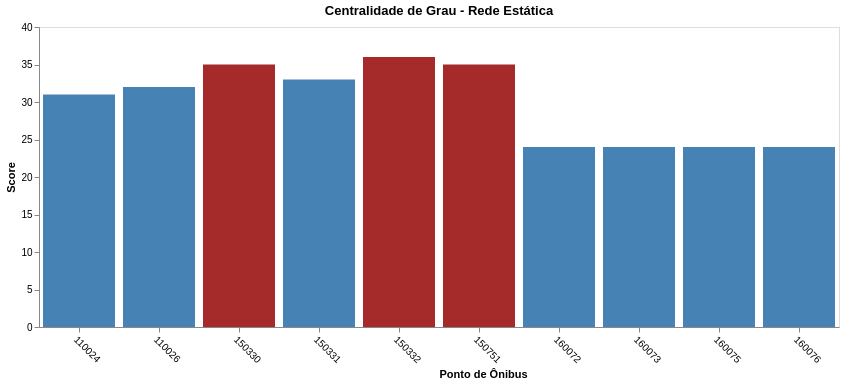
\includegraphics[width=.9\textwidth]{Capitulo4/img/centralidade-grau.png}
\caption{Centralidade de grau da rede estática.}
\label{fig:eventos-de-proximidade}
\end{figure}

\begin{figure}
\centering
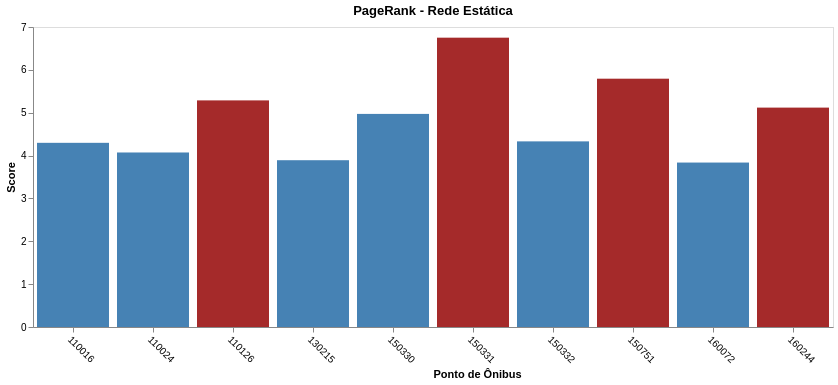
\includegraphics[width=.9\textwidth]{Capitulo4/img/pagerank.png}
\caption{PageRank da rede estática.}
\label{fig:eventos-de-proximidade}
\end{figure}


\begin{figure}
\centering
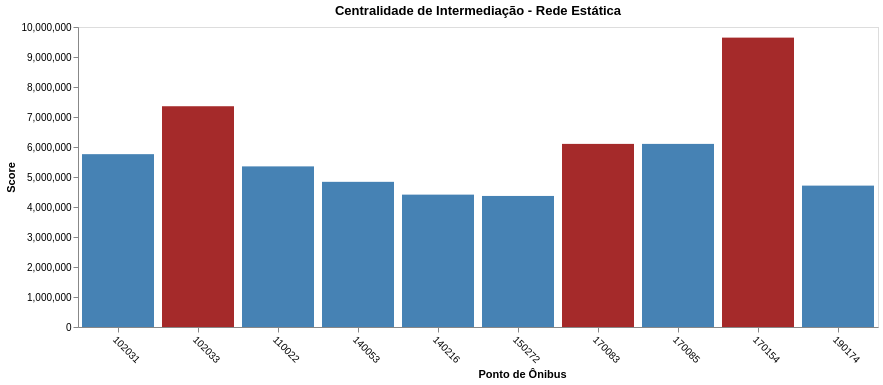
\includegraphics[width=.9\textwidth]{Capitulo4/img/centralidade-intermediacao.png}
\caption{Centralidade de Intermediação.}
\label{fig:eventos-de-proximidade}
\end{figure}



% Integração Temporal
% Os passageiros do transporte coletivo de Curitiba têm diferentes tipos de integração temporal para trocar de linha de ônibus ou de estação-tubo sem precisar pagar nova tarifa. Em 2017 foram mais de 600 mil usos nas integrações temporais das linhas urbanas da capital. Se contar o acesso às Ruas da Cidadania, esse atendimento sobe para quase um milhão.

% A proposta das integrações temporais no transporte é oferecer uma alternativa aos passageiros que ainda não têm acesso à integração no sistema. No transporte da capital, uma pessoa embarca num ponto e percorre todos os 21 terminais e as mais de 300 estações-tubo pagando apenas uma tarifa. Isso ocorre em 92\% da rede de transporte da cidade. A integração temporal busca complementar gradativamente essa rede.

% O único critério para usar a integração temporal é ter o cartão-transporte da URBS, que permite também o acesso às Ruas da Cidadania, onde o passageiro economiza uma tarifa no retorno ao ônibus. Veja quais são os tipos de integrações possíveis:

% Para o usuário ter direito à integração temporal, o mesmo deve utilizar o cartão-transporte da URBS em um dos validadores do Sistema de Transporte Coletivo de Curitiba (Ônibus, Terminal, Estação-Tubo), realizando assim um debito de passagem do seu Cartão Transporte e conforme as regras abaixo.

% OBS.: apenas os cartões-transporte nas modalidades Usuário e Estudante realizam integração temporal. Com o cartão-transporte Avulso não há a possibilidade de uso do benefício da integração temporal.


 
 
%\ric{Cada resultado precisa ser explicado.}

% A Figura~\ref{fig:centralidade-grau-estatica} mostra a centralidade de grau considerando apenas os pontos de ônibus (rede estática, ou seja, sem movimentação de ônibus). Os pontos 150331, 110026 e 150332 são os pontos de maior centralidade de grau, ou seja, conectam um número maior de pontos de ônibus devido a um maior número de linhas que passam por estes pontos. Em Curitiba, enquanto que o segundo ponto localiza-se na região central da cidade, os dois outros pontos (150331 e 150332) localizam-se na região sul da cidade. Em todos os casos, são pontos para onde convergem várias linhas de ônibus antes de chegarem a terminais importantes da cidade (terminal Pinheirinho ao sul, nos caso dos pontos 150331 e 150332, e praça Rui Barbosa no centro, no caso do ponto 110026). 
%Cabe ressaltar que a rede complexa construída considera pontos distintos, mesmo em terminais de ônibus, seguindo representação da URBS.

%{\bf Resultado 1:} Grau dos nós (\emph{Bus Stop}) para a rede estática (sem \emph{Stops}) na forma de histograma para os 10 nós de maior grau;

% \begin{figure}
% \centering
% \includegraphics[width=.9\textwidth]{fig/fig5.png}
% \caption{Centralidade de grau para pontos de ônibus (dez maiores) sem movimentação de ônibus (rede estática).}
% \label{fig:centralidade-grau-estatica}
% \end{figure}

% A Figura~\ref{fig:centralidade-grau-dinamica} mostra a centralidade de grau considerando as paradas de ônibus nos pontos de ônibus ao longo do dia (rede dinâmica, ou seja, com movimentação de ônibus). São mostrados os resultados para os três pontos de maior centralidade de grau da rede estática (150331, 110026 e 150332). Nota-se uma maior concentração no período da manhã e meio do dia, com diminuição gradual até o final da noite. Ao mesmo tempo, o ponto 150331 atende um elevado número de ônibus no período da manhã e no final da tarde. Essa última característica ocorre em Curitiba por conta do encerramento de atividades em empresas (trabalhadores retornando a suas casas) e estudantes de ensino noturno se deslocando para instituições de ensino.

%{\bf Resultado 2:} Evolução ao longo do dia do grau dos top 3 nós (\emph{Bus Stop}) anteriores;


% \begin{figure}
% \centering
% \includegraphics[width=.9\textwidth]{fig/fig7.png}
% \caption{Centralidade de grau para pontos de ônibus (três maiores) com movimentação de ônibus ao longo do dia (rede dinâmica)}
% \label{fig:centralidade-grau-dinamica}
% \end{figure}


% A Figura~\ref{fig:pagerank} mostra o \emph{page rank} considerando apenas a rede estática (pontos de ônibus). Os pontos 150331, 110026 e 110016 são os pontos de maior \emph{page rank}. Estes pontos se localizam, respectivamente, na região sul da cidade (na saída do terminal Pinheirinho), na região que conecta o centro a região nordeste da cidade (na direção de terminais Cabral, Boa Vista e Santa Cândida), nas proximidades do centro da cidade. Todos esses pontos conectam várias linhas que se afastam (pontos 150331 e 110126) ou se aproximam (ponto 11016) de regiões de grande concentração de pontos finais de linhas de ônibus. Ou seja, a importância destes pontos se deve a ligações com outros pontos importantes (pontos ou terminais com grande concentração de linhas).

%Lembrando que esta métrica indica relevância de pontos em relação aos demais pontos que se conectam a eles: são pontos importantes porque outros pontos significativos estão conectados, por linhas de ônibus, a eles.}

%{\bf Resultado 3:} \emph{PageRank} dos nós (\emph{Bus Stop}) para a rede estática (sem \emph{Stops}) na forma de histograma para os 10 nós de maior \emph{rank};

% \begin{figure}
% \centering
% \includegraphics[width=.9\textwidth]{fig/fig8.png}
% \caption{\emph{Page rank} para pontos de ônibus (dez maiores) sem movimentação de ônibus (rede estática).}
% \label{fig:pagerank}
% \end{figure}

%%%% Comentado por falta de espaço

% A Tabela~\ref{tab:n_linhas} mostra a comparação entre os três vértices de maior centralidade de grau (150332, 150331 e 110026) e os três vértices de maior \emph{page rank} (150331,150751,160244). \mar{Assim que os valores de grau forem recolocados, cabe um comentário sobre relação grau x page rank.}

% \begin{table}[h]
%     \caption{Comparação entre centralidade de grau  e \emph{page rank.}}
%     \label{tab:n_linhas}
%     \centering
%     \begin{tabular}{cccc} 
%         \hline
%         Ponto & Centralidade de grau & \emph{Page rank} \\
%         \hline
%         150332 & 63  & 4.15 \\
%         110026 & 64  &  3.75 \\
%         150751 & 63  & {\bf 5.53 } \\
%         150331 & 65  & {\bf 6.58} \\
%         160244 & 40  & {\bf4.82} \\
%         150330 &  32 &  4.75 \\
%         \hline 
        
%     \end{tabular}
% \end{table}

% \begin{table}[h]
%     \caption{Comparação entre Centralidade de grau  e \emph{page rank.}}
%     \label{tab:n_linhas}
%     \centering
%     \begin{tabular}{ccccc} 
%         \hline
%         Ponto & No. linhas & Centralidade de Grau & \emph{Page Rank} \\
%         \hline
%         110026 & 27  & 23 &  3.91 \\
%         150332 & 24  & 32 & 2.21 \\
%         150331 & 24  & 27 & {\bf 6.01} \\
%         110126 & 18  & 21 &  {\bf 5.50} \\
%         110016 & 16  & 11 & {\bf 4.57}\\
        
%         \hline  
%     \end{tabular}
% \end{table}

% As medidas de comprimento das linhas da rede estática de transporte resultaram em 40~m, 38,14~km e 9,43~km para os comprimentos mínimo, máximo e médio (com desvio padrão de 6,5~km) das linhas de ônibus. Já as medidas baseadas em caminhos mínimos entre pontos da rede resultaram em um valor mínimo de 3,6~m, diâmetro da rede (caminho mínimo mais longo) de 55~km e um percurso médio de 14,04~km. Estes caminhos mínimos foram obtidos através dos atributos de distância (\texttt{DISTANCE}) das arestas \texttt{NEXT\_STOP}, gerando uma rede ponderada do sistema de transporte de Curitiba. Note que esse percurso médio pode ou não ser factível com troca de ônibus (baldeação), dependendo da origem e destino do passageiro.
%Tais métricas são úteis para comparação entre sistemas de transporte de diferentes cidades, e para planejamento do próprio sistema, seja na redução de distância ou no tempo de percurso dos passageiros.

%{\bf Resultado 5:} Tabela de medidas da rede estática: comprimento mínimo, máximo e médio das linhas (em km); média dos caminhos mínimos (de cada nó para todos os outros; diâmetro da rede (caminho mínimo mais longo);


% \begin{table}[h]
%     \caption{Comprimento das linhas de ônibus e diâmetro da rede estática (km).}
%     \label{tab:medidas}
%     \centering
%     \begin{tabular}{cccc} 
%         \hline
%       Mínimo &Máximo &Médio (desv. padrão) &Diâmetro\\
%         \hline
%         0,04 & 38,14  & 9,43 (6,5) & xxx \\
%         \hline  
%     \end{tabular}
% \end{table}

% A Figura~\ref{fig:betweeness} mostra a centralidade de intermediação considerando apenas a rede estática (pontos de ônibus). Os pontos 170154, 170085 e 170083 são os pontos de maior centralidade de intermediação. Estes pontos localizam-se na vizinhança do terminal Pinheirinho, localizado na parte sul de Curitiba, comportando-se como um \emph{hub} por onde passam percursos mais curtos entre pontos de ônibus da rede. Note também que esses percursos podem ou não ser factíveis com trocas de ônibus.
%Eles refletem indiretamente a movimentação de pessoas dessa região da cidade (basicamente bairros-dormitórios) para trabalharem ou estudarem nas demais partes da cidade, ou seja, a uma relação desses resultados com a evolução urbana da cidade.

%{\bf Resultado 6:} Centralidade de intermediação (\emph{betweenness}) - ver depois.

% \begin{figure}
% \centering
% \includegraphics[width=.9\textwidth]{fig/fig9.png}
% \caption{Centralidade de intermediação para pontos de ônibus (dez maiores) sem movimentação de ônibus (rede estática).}
% \label{fig:betweeness}
% \end{figure}


% \begin{table}[h]
%     \caption{PageRank 07:00 - 10:00 02/05/2019}
%     \centering
%     \begin{tabular}{llll} 
%         \hline
%         ID Ponto	 &No. linhas &No. paradas &PageRank  \\
%         \hline
%         150751 &24 &1440 &2.74556 \\
%         150331 &24 &1152 &3.43579 \\
%         110026 &26 &704  &2.68251 \\
%         110024 &26 &496  &2.89234 \\
%         150635 &14 &418  &2.67968 \\
%         160244 &17 &160  &2.88967 \\
%         190199 &7  &143  &2.69128 \\
%         150203 &5  &143  &2.63893 \\
%         120020 &8  &72   &2.76218 \\ 
%         190198 &6  &9	 &2.75211 \\
%         \hline 
%     \end{tabular}
%     \label{tab:res_pagerank_07_10}
% \end{table}



% \begin{table}[h]
%     \caption{PageRank 07:00 - 10:00 02/05/2019}
%     \centering
%     \begin{tabular}{ llllll } 
%         \hline
%         Nº doPonto	 & Nome do Ponto &	linhas & N° Veículos & Nº Paradas &	PageRank  \\
%         \hline
%         150751 & 	Av. Winston Churchill, 2677     &	24 & 21 & 1440 & 2.74556 \\
%         150331 &	 Av. Winston Churchill, 2472    &	24 & 19	& 1152 & 3.43579 \\
%         110026 &	 Rua Alferes Poli, 400          &	26 & 16	& 704  & 2.68251 \\
%         110024 &	 Rua Alferes Poli, 787          &	26 & 13	& 496  & 2.89234 \\
%         150635 &	 Av. Pres. Getulio Vargas, 2676 &	14 & 15	& 418  & 2.67968 \\
%         160244 &	 Rua Emanoel Voluz, 284         &	17 & 5	& 160  & 2.88967 \\
%         190199 &	 Marginal Rodovia BR- 277, 926  & 	7  & 6	& 143  & 2.69128 \\
%         150203 &	 Rua Alcino Guanabara, 1237     & 	5  & 7	& 143  & 2.63893 \\
%         120020 &	 Av. Anita Garibaldi, 3431      &	8  & 6	& 72   & 2.76218 \\ 
%         190198 &	 Marginal Rodovia BR- 277, 926  &	6  & 1	& 9	   & 2.75211 \\
%         \hline 
%     \end{tabular}
%     \label{tab:res_pagerank_07_10}
% \end{table}


% \begin{table}[h]
%     \caption{PageRank 12:00 - 14:00 02/05/2019}
%     \centering
%     \begin{tabular}{ llllll } 
%         \hline
%         Nº do Ponto	 & Nome do Ponto &	linhas & N° Veículos & Nº Paradas &	PageRank  \\
%         \hline
%         150751 & Av. Winston Churchill, 2677      &	24	& 21 & 1440 & 2.64988  \\
%         150331 & Av. Winston Churchill, 2472      &	24	& 19 & 1152	& 2.85910  \\
%         110026 & Rua Alferes Poli, 400	          & 26	& 16 & 704	& 2.47933  \\
%         110024 & Rua Alferes Poli, 787	          & 26	& 13 & 496	& 2.64934  \\
%         160244 & Rua Emanoel Voluz, 284 	      & 17	& 5	 & 160	& 2.79724  \\
%         180020 & Rua Rezala Simão, 997            &	 7	& 6	 & 143	& 2.95418  \\
%         190199 & Marginal Rodovia BR- 277, 926    &  7	& 6	 & 143	& 2.42175  \\
%         150203 & Rua Alcino Guanabara, 1237       &	 5	& 7	 & 143	& 2.38609  \\
%         150070 & Rua Maria Trevisan Tortato, 642  &  7	& 3	 & 52	& 3.02172  \\
%         180007 & R. Carlos Klemtz, 1000           &	 7	& 4	 & 52	& 2.72499 \\
%         \hline 
%     \end{tabular}
%     \label{tab:res_pagerank_12_14}
% \end{table}


% \begin{figure}
% \centering
% \includegraphics[width=.9\textwidth]{fig/fig2.png}
% \caption{Evolução horária do grau da rede do sistema de transporte no dia 02/05/2019}
% \label{fig:grau}
% \end{figure}


% \begin{figure}
% \centering
% \includegraphics[width=.9\textwidth]{fig/fig3.png}
% \caption{nº de veículos no dia 02/05/2019}
% \label{fig:veiculos}
% \end{figure}



\section{Integração temporal}

%%%%%% O que está abaixo não necessariamente permanecerá no texto - por enquanto é apenas uma referência para a seção

\ric{Resumo da metodologia}

\begin{enumerate}
    \item Para cada ponto de ônibus, obtém-se uma série temporal com o número de eventos (paradas de ônibus) em uma janela deslizante de 10 min, calculada minuto a minuto ao longo do período considerado (0 a 24 horas?);
    \item Identificam-se os 10 pontos (centroides) mais bem servidos em termos do número de eventos agregados para todos o período considerado;
    \item Para cada centroide, selecionam-se os pontos a uma distância de 600~m do centroide e gera-se uma matriz de correlação entre as séries temporais de cada ponto desta região;
    \item Identificam-se os pontos de maior correlação (com o centroide?);
    \item Estes pontos serão os candidatos para estabelecer integração temporal.
\end{enumerate}

\ric{Resultados a serem apresentados sobre o levantamento de regiões candidatas para integração temporal:}

\begin{itemize}
    \item Visualização das regiões estudadas (centroides) no mapa de Curitiba;
    \item Número de pontos e raio médio destas regiões, ou seja, os pontos selecionados estão em um raio muito menor do que 600~m?
    \item Quantas linhas de ônibus servem cada região? Elas se conectam em algum outro ponto da rede, ou seja, existe um terminal ou estação tubo onde a transferência possa ser realizada ser pagamento de nova tarifa?
    \item Dar especial atenção aos centroides que "integram" várias linhas (Alferes Poli?; Centro Cívico?); estes centroides, além de possuírem serviços "sincronizados" (precisa definir o que seria isso), permitem criar novas rotas;
\end{itemize}

\ric{Resultados a serem apresentados sobre o impacto na rede da implementação da integração temporal para as regiões selecionadas:}

\begin{itemize}
    \item Tem impacto na métrica de redes complexas (centralidade de proximidade ou intermediação, diâmetro)?
\end{itemize}%% Comente para remover este item

%% Parte
% \part{Conclusão}%% Comente para remover este item

%% Capítulo
%%%% CAPÍTULO 5 - CONCLUSÕES E PERSPECTIVAS
%%
%% Deve finalizar o trabalho com uma resposta às
%% hipóteses especificadas na introdução. O autor deve
%% manifestar seu ponto de vista sobre os resultados
%% obtidos; não se deve incluir neste capítulo novos
%% dados ou equações. A partir da tese, alguns assuntos
%% que foram identificados como importantes para serem
%% explorados poderão ser sugeridos como temas para
%% novas pesquisas.

%% Título e rótulo de capítulo (rótulos não devem conter caracteres especiais, acentuados ou cedilha)
\chapter{Conclusões e Perspectivas}\label{cap:conclusoeseperspectivas}

% Deve finalizar o trabalho com uma resposta às hipóteses especificadas na introdução. O autor deve manifestar seu ponto de vista sobre os resultados obtidos; não se deve incluir neste capítulo novos dados ou equações. A partir da tese, alguns assuntos que foram identificados como importantes para serem explorados poderão ser sugeridos como temas para novas pesquisas.

\ric{Algumas questões para abordar na conclusão:}
\begin{enumerate}
    \item Esta metodologia poderia ser utilizada para propor novos terminais? Parece que a metodologia para construir novos terminais de ônibus não é muito consolidada;
\end{enumerate}

Este trabalho propôs uma plataforma computacional para construção automática de um banco de dados de grafo a partir de um repositório de dados abertos com informações da operação diária do transporte de Curitiba. O modelo utilizado corresponde a um grafo variante no tempo (TVG) disponível na literatura com poucas modificações. A plataforma computacional transforma dados brutos do repositório para a base de dados de grafos do Neo4j. Diversos algoritmos de análise de redes complexas podem então ser aplicados. Resultados de centralidade de grau, \emph{page rank} e centralidade de intermediação permitiram identificar pontos de ônibus relevantes na rede, seja pela concentração de linhas (rede estática, sem movimentação de ônibus) ou paradas de ônibus (rede dinâmica, considerando a movimentação de ônibus), além de características dos caminhos da rede. Estas medidas são úteis para o planejamento do transporte, pois permitem avaliar a área coberta e a frequência e regularidade dos serviços. Esta última é particularmente importante no estabelecimento da integração temporal das linhas, quando uma tarifa é válida por um determinado período de tempo em toda ou parte da rede de transporte. Embora os resultados de análise tenham sido apresentados para o sistema de transporte de Curitiba, o modelo pode ser adaptado para o transporte de ônibus de outras cidades. Como trabalhos futuros pode-se incluir o tratamento de regiões geográficas para análises de bairros ou outros agrupamentos georreferenciados. Da mesma forma, a inclusão de informações de arruamento baseado no \emph{OpenStreetMap} permitirá relacionar a operação do transporte às vias de circulação da cidade.
%% Comente para remover este item

%% Capítulos após este comando criam marcadores do pdf na raiz
% \phantompart%% Comente para remover este item

%% Capítulo de exemplo
% %%%% CAPÍTULO - EXEMPLO
%%
%% Capítulo de informações e exemplos de utilização deste modelo.
%%
%% Criado por Luiz E. M. Lima (UTFPRPG-TEX) e adaptado para o contexto da UTFPRCT-TEX por William H. T. Meira

%% Título e rótulo de capítulo (rótulos não devem conter caracteres especiais, acentuados ou cedilha)
\chapter{Informações e Exemplos de Utilização deste Modelo}\label{cap:exemplo}

Devido à necessidade de padronização em trabalhos acadêmicos (teses, dissertações, trabalhos de conclusão de curso, etc.), são utilizadas neste documento algumas regras básicas para estruturação e formatação.

Deste modo, o presente documento foi produzido utilizando o modelo \gls{utfprcttex}\index{UTFPRCTTeX@\utfprcttex} para elaboração de trabalhos acadêmicos segundo as normas definidas pela \gls{utfpr}\index{UTFPR} \cite{UTFPR2017}. Este modelo foi desenvolvido em linguagem de editoração \gls{tex}\index{TeX@\TeX}/\gls{latex}\index{LaTeX@\latex} com base no modelo \gls{utfprpgtex}\index{UTFPRPGTEX@\utfprpgtex} \cite{LIMA2019} mantido por Luiz E. M. Lima. Por sua vez, a base de ambos os modelos é o \gls{abntex2}\index{abnTeX2@\abnTeX} \cite{abnTeX2:2013}, que atende os requisitos das normas da \gls{abnt}\index{ABNT} para elaboração de documentos técnicos e científicos brasileiros.

Os arquivos principais do modelo \gls{utfprcttex}\index{UTFPRCTTeX@\utfprcttex} são: \texttt{utfprct.tex} e \texttt{utfprct-dados.tex}. O segundo tem por finalidade a definição de informações sobre o documento, o autor, o orientador, o coorientador, a instituição e a defesa do trabalho. O primeiro constitui a estrutura central deste modelo e tem por finalidade:

\begin{itemize}%% Lista de itens
\item Definir a classe e as opções do documento.
\item Permitir o carregamento de pacotes adicionais.
\item Permitir a definição de comandos personalizados.
\item Permitir a inclusão de arquivos auxiliares, por exemplo, fontes de dados do documento e elementos pré-textuais, textuais e pós-textuais.
\end{itemize}

A codificação de caracteres em todos os arquivos é \texttt{UTF8}, tanto no modelo \gls{abntex2}\index{abnTeX2@\abnTeX} quanto no modelo \gls{utfprcttex}\index{UTFPRCTTeX@\utfprcttex}. Portanto, é necessário que seja utilizada a mesma codificação nos documentos a serem desenvolvidos, inclusive nos arquivos de base bibliográfica. Diversos editores de arquivos fonte do \gls{latex}\index{LaTeX@\latex} são capazes de manipular e/ou converter entre diferentes codificações, por exemplo, o ``Texmaker\index{Texmaker}'' (disponível em \url{http://www.xm1math.net/texmaker/}). Recomenda-se, sempre que for manipular e/ou substituir um dos arquivos constituintes deste modelo, manter uma cópia do original num local seguro e/ou renomear esta cópia do original para que possa ser utilizada como um exemplo no desenvolvimento do seu próprio arquivo. Por exemplo, quando for criar o seu ``Capítulo 1'', fazer uma cópia do arquivo original \texttt{capitulo1.tex}, renomeando-o para \texttt{capitulo1.original.tex}, por exemplo, e realizar as alterações e/ou modificações no arquivo \texttt{capitulo1.tex}.

Este capítulo\label{errata:capitulo} de exemplo tem por finalidade a definição e a apresentação de alguns comandos do \gls{latex}\index{LaTeX@\latex} e/ou dos modelos \gls{abntex2}\index{abnTeX2@\abnTeX} e \gls{utfprcttex}\index{UTFPRCTTeX@\utfprcttex}. O presente documento não se constitui um manual, tampouco uma apostila de \gls{latex}\index{LaTeX@\latex}, visto que existe uma grande quantidade de material de referência disponível na internet, como por exemplo em \url{http://en.wikibooks.org/wiki/LaTeX}.

Os capítulos devem conter uma introdução e um fecho. A introdução fornece ao leitor uma breve descrição do que será tratado no capítulo, enquanto o fecho apresenta comentários finais sobre o que foi desenvolvido no capítulo. Os capítulos podem ser divididos em seções\label{errata:secao}. Esta divisão deve ser lógica (temática) e não física (por tamanho). O número ideal de seções é impossível de se precisar. Entretanto, um capítulo com uma única seção, possivelmente, deverá ser agregado ao capítulo anterior ou posterior. Um capítulo com quinze seções, possivelmente, deverá ser subdividido em dois capítulos. Capítulos, seções e subseções\label{errata:subsecao} devem ser rotulados para que possam ser referenciados em qualquer parte do texto. Exemplo: O \autoref{cap:exemplo} é gerado, rotulado e referenciado pelos comandos \verb|\chapter{Informações e...}|, \verb|\label{cap:exemplo}| e \verb|\autoref{cap:exemplo}|, respectivamente.

%% Título e rótulo de seção (rótulos não devem conter caracteres especiais, acentuados ou cedilha)
\section{Título da Seção Secundária}\label{sec:secsec}

Seções secundárias são divisões do conteúdo das seções primárias. A \autoref{sec:secsec} é gerada, rotulada e referenciada pelos comandos \verb|\section{Título da Seção Secundária}|, \verb|\label{sec:secsec}| e \verb|\autoref{sec:secsec}|, respectivamente.

%% Título e rótulo de seção (rótulos não devem conter caracteres especiais, acentuados ou cedilha)
\subsection{Título da Seção Terciária}\label{ssec:secterc}

Seções terciárias são divisões do conteúdo de seções secundárias. A \autoref{ssec:secterc} é gerada, rotulada e referenciada pelos comandos \verb|\subsection{Título da Seção Terciária}|, \verb|\label{ssec:secterc}| e \verb|\autoref{ssec:secterc}|, respectivamente.

%% Título e rótulo de seção (rótulos não devem conter caracteres especiais, acentuados ou cedilha)
\subsubsection{Título da seção quartenária}\label{sssec:secquart}

Seções quartenárias são divisões do conteúdo de seções terciárias. A \autoref{sssec:secquart} é gerada, rotulada e referenciada pelos comandos \verb|\subsubsection{Título da seção quartenária}|, \verb|\label{sssec:secquart}| e \verb|\autoref{sssec:secquart}|, respectivamente.

%% Título e rótulo de seção (rótulos não devem conter caracteres especiais, acentuados ou cedilha)
\paragraph{Título da seção quinária}\label{par:secqui}

Seções quinárias são divisões do conteúdo de seções quartenárias. A \autoref{par:secqui} é gerada, rotulada e referenciada pelos comandos \verb|\paragraph{Título da seção quinária}|, \verb|\label{par:secqui}| e \verb|\autoref{par:secqui}|, respectivamente.

%% Título e rótulo de seção (rótulos não devem conter caracteres especiais, acentuados ou cedilha)
\section{Exemplo de Título de Seção Secundária com um Texto Muito Longo que Pode Ocupar Mais de uma Linha}\label{sec:sectitulolongo}

A \autoref{sec:sectitulolongo} é um exemplo de título de seção secundária com texto muito longo, formatado automaticamente de acordo com \citeonline[subseções~5.2.2 a 5.2.4]{NBR14724:2011} e \citeonline[subseções~3.1 a 3.8]{NBR6024:2012}. Segundo as normas, o título de seção deve estar alinhado à esquerda e a segunda e demais linhas devem iniciar logo abaixo da primeira palavra da primeira linha.

%% Título e rótulo de seção (rótulos não devem conter caracteres especiais, acentuados ou cedilha)
\section{Elementos Pré-Textuais}\label{sec:elempretext}

Alguns elementos pré-textuais do presente documento são gerados automaticamente pelo \gls{utfprcttex}\index{UTFPRCTTeX@\utfprcttex}. Para adicionar e/ou alterar as informações apresentadas na capa, na folha de rosto, na ficha catalográfica e na folha de aprovação deve-se editar o arquivo \texttt{utfprct-dados.tex}. Os dados informados neste arquivo também são utilizados para gerar a referência do trabalho na errata, no resumo e no \textit{abstract}. Podem ser adicionados informações de cotutela (ou duplo grau) da instituição externa para serem apresentados nos elementos pré-textuais.

Para adicionar e/ou alterar o texto da errata, da dedicatória, dos agradecimentos, da epígrafe, do resumo e do \textit{abstract} deve-se editar seus respectivos arquivos presentes no diretório ``PreTexto'': \texttt{errata.tex}, \texttt{dedicatoria.tex}, \texttt{agradecimentos.tex}, \texttt{epigrafe.tex}, \texttt{resumo.tex} e \texttt{abstract.tex}.

As listas de algoritmos, de ilustrações e de tabelas são geradas automaticamente pelo \gls{utfprcttex}\index{UTFPRCTTeX@\utfprcttex}. Os itens destas listas são gerados a medida que forem sendo inseridos no texto do documento. A lista de abreviaturas, siglas e acrônimos pode ser gerada automaticamente através do arquivo \texttt{entradas-acronimos.tex}, utilizando o pacote \texttt{glossaries}\footnote{Detalhes sobre comandos para geração de abreviaturas, siglas e acrônimos utilizando o pacote \texttt{glossaries} são apresentadas na \autoref{sec:acronimos}.}, ou através da edição do arquivo \texttt{lista-acronimos.tex}. A lista de símbolos pode ser gerada automaticamente utilizando o pacote \texttt{nomencl}\footnote{Detalhes sobre comandos para geração de símbolos utilizando o pacote \texttt{nomencl} são apresentadas na \autoref{sec:simbolos}.} ou através da edição do arquivo \texttt{lista-simbolos.tex}. Os arquivos citados estão no diretório ``PreTexto''. O sumário é o último elemento pré-textual e também é gerado automaticamente pelo \gls{utfprcttex}\index{UTFPRCTTeX@\utfprcttex}.

%% Título e rótulo de seção (rótulos não devem conter caracteres especiais, acentuados ou cedilha)
\section{Regras Gerais de Apresentação}\label{sec:regrasgerais}

As regras gerais de apresentação, definidas na sequência, já estão predefinidas no modelo \gls{utfprcttex}\index{UTFPRCTTeX@\utfprcttex}. Algumas destas regras podem ser alteradas, por comandos apropriados do \gls{latex}\index{LaTeX@\latex}, do \gls{abntex2}\index{abnTeX2@\abnTeX} ou do \gls{utfprcttex}\index{UTFPRCTTeX@\utfprcttex}, no preâmbulo do arquivo principal \texttt{utfprcttex.tex} ou em outras partes do documento, por exemplo, nos capítulos.

\begin{itemize}%% Lista de itens
\item Configuração das margens: deve-se usar margens superior e esquerda de \SI{3}{cm}; e margens inferior e direita de \SI{2}{cm}; em papel formato A4 ($\SI{21}{cm} \times \SI{29,7}{cm}$).
\item Recomenda-se o uso de fonte tipo Arial ou Times New Roman, tamanho 12 para o texto e tamanho 10 para citações de mais de três linhas, notas de rodapé e legendas dos algoritmos, ilustrações e tabelas.
\item O parágrafo deve aparecer com recuo na primeira linha de \SI{1,5}{cm}, justificado, sem espaçamento anterior ou posterior.
\item Os elementos como: o resumo, as notas, as referências, as legendas das ilustrações e tabelas, a natureza do trabalho, o objetivo, o nome da instituição a que é submetida e a área de concentração devem ser digitados em espaço simples.
\item A numeração progressiva para as seções do texto deve ser adotada para evidenciar a sistematização do conteúdo do trabalho.
\item Para os títulos das seções não se utilizam pontos, hífen, travessão, ou qualquer sinal após o indicativo de seção ou de título.
\item Para as seções primárias: utiliza-se negrito e caixa alta.
\item Para as seções secundárias: somente caixa alta e sem negrito.
\item Para as seções terciárias: a primeira letra de cada palavra em maiúscula (desconsidera-se artigos e preposições).
\item Para as seções quaternárias: somente a primeira letra do título da seção em maiúscula.
\item No sumário, os títulos das seções devem aparecer exatamente iguais ao que estão contidos no trabalho.
\end{itemize}

Recomenda-se evitar, sempre que possível, o uso dos seguintes recursos (ou enfeites) no documento:

\begin{itemize}%% Lista de itens
\item \textbf{o uso de negrito;}
\item \textit{o uso de itálico (exceto em palavras em outra língua);}
\item \texttt{texto em diferente fonte como máquina de escrever;}
\item \underline{o uso de texto sublinhado;}
\item o uso excessivo de\footnote{Notas de rodapé.}.
\end{itemize}

\noindent Lembre-se: um texto ``limpo'' é mais agradável de ler que um texto ``enfeitado''.

%% Título e rótulo de seção (rótulos não devem conter caracteres especiais, acentuados ou cedilha)
\subsection{Espaçamento}\label{sec:espacamento}

\begin{itemize}%% Lista de itens
\item O resumo, o \textit{abstract}, as notas, as referências, as legendas das ilustrações e tabelas e a natureza do trabalho devem ser digitadas em espaço simples.
\item Todo o texto deve ser formatado com espaço entre linhas de um fator de 1,5 (sem espaçamento antes/depois).
\item As citações com mais de três linhas devem ser em espaço simples e com recuo de \SI{4}{cm} da margem esquerda.
\item As referências, ao final do trabalho, devem ser separadas entre si por um espaço simples, e na mesma referência o espaço é simples \cite{NBR6023:2018}.
\item Os títulos das seções secundárias devem ser separados do texto que os precede por dois espaços entre linhas de um fator de 1,5.
\item As seções primárias devem iniciar em páginas distintas.
\end{itemize}

O recuo na primeira linha, espaço entre a margem e o início do parágrafo, pode ser redefinido definido pelo comando:

\begin{SingleSpacing}%% Ambiente SingleSpacing
\begin{verbatim}
\setlength{\parindent}{1.5cm}
\end{verbatim}
\end{SingleSpacing}

O espaçamento entre um parágrafo e outro\index{espaçamento!entre os parágrafos} pode ser redefinido pelo comando:

\begin{SingleSpacing}%% Ambiente SingleSpacing
\begin{verbatim}
\setlength{\parskip}{0mm} %% Tente também \onelineskip
\end{verbatim}
\end{SingleSpacing}

O controle do espaçamento entre linhas\index{espaçamento!entre as linhas} pode ser redefinido pelo comando:

\begin{SingleSpacing}%% Ambiente SingleSpacing
\begin{verbatim}
\OnehalfSpacing %% Espaçamento um e meio (padrão)
\DoubleSpacing  %% Espaçamento duplo
\SingleSpacing  %% Espaçamento simples
\end{verbatim}
\end{SingleSpacing}

Para isso, também estão disponíveis os ambientes:

\begin{SingleSpacing}%% Ambiente SingleSpacing
\begin{verbatim}
\begin{SingleSpacing} ...     \end{SingleSpacing}
\begin{Spacing}{<factor>} ... \end{Spacing}
\begin{OnehalfSpacing} ...    \end{OnehalfSpacing}
\begin{OnehalfSpacing*} ...   \end{OnehalfSpacing*}
\begin{DoubleSpacing} ...     \end{DoubleSpacing}
\begin{DoubleSpacing*} ...    \end{DoubleSpacing*}
\end{verbatim}
\end{SingleSpacing}

Para mais informações, consulte \citeonline[p.~47-52 e 135]{Wilson2010}.

%% Título e rótulo de seção (rótulos não devem conter caracteres especiais, acentuados ou cedilha)
\section{Enumerações: Alíneas e Subalíneas}\label{sec:enumeracoes}\index{alíneas}\index{subalíneas}

Quando for necessário enumerar os diversos assuntos de uma seção que não possua título, esta deve ser subdividida em alíneas\index{alíneas} \cite[subseção~4.2]{NBR6024:2012}:

\begin{alineas}%% Ambiente alineas
\item os diversos assuntos que não possuam título próprio, dentro de uma mesma seção, devem ser subdivididos em alíneas\index{alíneas};
\item o texto que antecede as alíneas\index{alíneas} termina em dois pontos;
\item as alíneas\index{alíneas} devem ser indicadas alfabeticamente, em letra minúscula, seguida de parêntese. Utilizam-se letras dobradas, quando esgotadas as letras do alfabeto;
\item as letras indicativas das alíneas\index{alíneas} devem apresentar recuo em relação à margem esquerda;
\item o texto da alínea deve começar por letra minúscula e terminar em ponto-e-vírgula, exceto a última alínea que termina em ponto final;
\item o texto da alínea deve terminar em dois pontos, se houver subalínea;
\item a segunda e as seguintes linhas do texto da alínea começa sob a primeira letra do texto da própria alínea;
\item subalíneas\index{subalíneas} \cite[subseção~4.3]{NBR6024:2012} devem ser conforme as alíneas\index{alíneas} a seguir:
\begin{alineas}%% Ambiente alineas
\item as subalíneas\index{subalíneas} devem começar por travessão seguido de espaço;
\item as subalíneas\index{subalíneas} devem apresentar recuo em relação à alínea;
\item o texto da subalínea deve começar por letra minúscula e terminar em ponto-e-vírgula. A última subalínea deve terminar em ponto final, se não houver alínea subsequente;
\item a segunda e as seguintes linhas do texto da subalínea começam sob a primeira letra do texto da própria subalínea.
\end{alineas}
\item no \gls{abntex2}\index{abnTeX2@\abnTeX} estão disponíveis os ambientes \texttt{incisos} e \texttt{subalineas}, que em suma são o mesmo que se criar outro nível de \texttt{alineas}, como nos exemplos à seguir:
\begin{incisos}%% Ambiente incisos
\item \textit{um novo inciso em itálico}\index{incisos}.
\end{incisos}
\item Alínea em \textbf{negrito}:
\begin{subalineas}%% Ambiente subalineas
\item \textit{uma subalínea em itálico};
\item \underline{\textit{uma subalínea em itálico e sublinhado}}.
\end{subalineas}
\item última alínea com \emph{ênfase}.
\end{alineas}

%% Título e rótulo de seção (rótulos não devem conter caracteres especiais, acentuados ou cedilha)
\section{Citações}\label{sec:citacoes}

O \gls{utfprcttex}\index{UTFPRCTTeX@\utfprcttex} está configurado para produzir as citações no texto no estilo alfabético (autor-ano), segundo as normas \gls{abnt}\index{ABNT}, através dos comandos do \gls{abntex2}\index{abnTeX2@\abnTeX} \cite{abnTeX2:2013Cite,abnTeX2:2013CiteAlf}. A lista dos principais comandos são apresentadas a seguir:

\begin{itemize}%% Lista de itens
\item \verb|\cite{rótulo}| -- para gerar citação implícita. Por exemplo, a citação ``\ldots\ \cite{Thompson2001}\ldots'' é gerada pelo comando \verb|\cite{Thompson2001}| ou pelo atalho \verb|\citep{Thompson2001}|, definido em \texttt{utfprcttex.tex}.
\item \verb|\citeonline{rótulo}| -- para gerar citação explícita. Por exemplo a citação ``\ldots\ conforme proposto por \citeonline{Thompson2001}\ldots'' é gerada pelo comando \verb|\citeonline{Thompson2001}| ou pelo atalho \verb|\citet{Thompson2001}|, definido em \texttt{utfprcttex.tex}.
\item \verb|(\citeauthor{rótulo})| -- para gerar citação implícita somente do autor. Por exemplo, a citação ``\ldots\ (\citeauthor{Thompson2001})\ldots'' é gerada pelo comando \verb|(\citeauthor{Thompson2001})| ou pelo atalho \verb|\citepa{Thompson2001}|, definido em \texttt{utfprcttex.tex}.
\item \verb|\citeauthoronline{rótulo}| -- para gerar citação explícita somente do autor. Por exemplo, a citação ``\ldots\ conforme a relação de \citeauthoronline{Thompson2001}\ldots'' é gerada pelo comando \verb|\citeauthoronline{Thompson2001}| ou pelo atalho \verb|\citeta{Thompson2001}|, definido em \texttt{utfprcttex.tex}.
\item \verb|(\citeyear{rótulo})| -- para gerar citação implícita somente do ano. Por exemplo, a citação ``\ldots\ (\citeyear{Thompson2001})\ldots'' é gerada pelo comando \verb|(\citeyear{Thompson2001})| ou pelo atalho \verb|\citepy{Thompson2001}|, definido em \texttt{utfprcttex.tex}.
\item \verb|\citeyear{rótulo}| -- para gerar citação explícita somente do ano. Por exemplo, a citação ``\ldots\ no ano de \citeyear{Thompson2001}\ldots'' é gerada pelo comando \verb|\citeyear{Thompson2001}| ou pelo atalho \verb|\citety{Thompson2001}|, definido em \texttt{utfprcttex.tex}.
\end{itemize}

Informações sobre a utilização dos comandos listados acima e os demais comandos para geração de referências, utilizados pelo \gls{abntex2}\index{abnTeX2@\abnTeX}, podem ser encontradas em \citeonline{abnTeX2:2013Cite,abnTeX2:2013CiteAlf}, disponíveis em \url{http://www.abntex.net.br/}.

\gls{latex}\index{LaTeX@\latex} utiliza um arquivo externo (em separado) para o banco de dados das referências citadas no texto. Este arquivo é compilado pelo \gls{bibtex}\index{BibTeX@Bib\TeX} e deve possuir a extensão \texttt{bib}, como nos arquivos \texttt{referencias.bib} e \texttt{referencias-modelos.bib} presentes no diretório ``PosTexto'', utilizados neste documento. O arquivo \texttt{exemplos-referencias.bib} apresenta exemplos dos seguintes estilos de referência aceitos pelo \gls{bibtex}\index{BibTeX@Bib\TeX}:

\begin{itemize}%% Lista de itens
\item anais de simpósios \citep{Alt1995,Pirmez2002};
\item artigos em anais de simpósios \citep{Faina2001};
\item artigos em coletâneas de artigos \citep{Pinto2000};
\item artigos em revistas \citep{Guimaraes2003};
\item capítulos de livros \citep{Santos2000};
\item livretos \citep{Thompson2001};
\item livros \citep{Pedrycz1998};
\item manuais técnicos \citep{IONA1999};
\item miscelânea \citep{Cruz2003};
\item páginas na internet \cite[acessado em 1 de janeiro de 2004]{Larsson2003} (utilizar a data do último acesso à página);
\item relatórios técnicos \citep{OMG2000};
\item teses de mestrado \citep{SantosFilho2003};
\item teses de doutorado \citep{Faina2000};
\item trabalhos não publicados \citep{Sichman2002}.
\end{itemize}

Existem alguns programas para gerenciamento de banco de dados de referências bibliográficas (arquivos \texttt{bib}) do \gls{bibtex}\index{BibTeX@Bib\TeX}. O ``JabRef'' é um exemplo destes programas e está disponível em: \url{http://jabref.sourceforge.net/}.

%% Título e rótulo de seção (rótulos não devem conter caracteres especiais, acentuados ou cedilha)
\subsection{Citações Diretas}\label{sec:citacoesdiretas}\index{citações!diretas}

O ambiente \texttt{citacao} permite a inclusão de citações diretas que ocupam mais de três linhas:

\begin{citacao}%% Ambiente citacao
As citações diretas no texto, que ocupam mais de três linhas, devem ser destacadas com recuo de \SI{4}{cm} da margem esquerda, com letra menor que a do texto utilizado e sem as aspas. No caso de documentos datilografados, deve-se observar apenas o recuo \cite[subseção 5.3]{NBR10520:2002}.
\end{citacao}

\noindent Esta citação direta com mais de três linhas foi gerada da seguinte forma:

\begin{SingleSpacing}%% Ambiente SingleSpacing
\begin{verbatim}
\begin{citacao}
As citações diretas no texto, com mais de três linhas,...
... observar apenas o recuo \cite[subseção~5.3]{NBR10520:2002}.
\end{citacao}
\end{verbatim}
\end{SingleSpacing}

O ambiente \texttt{citacao} pode receber como parâmetro opcional um nome de idioma previamente carregado nas opções da classe (definido no preâmbulo do arquivo \texttt{utfprcttex.tex}). Neste caso, o texto da citação é automaticamente escrito em itálico e a hifenização é ajustada para o idioma selecionado na opção do ambiente. Por exemplo:

\begin{SingleSpacing}%% Ambiente SingleSpacing
\begin{verbatim}
\begin{citacao}[english]
Text in English language in italic with correct hyphenation.
\end{citacao}
\end{verbatim}
\end{SingleSpacing}

\noindent Tem como resultado:

\begin{citacao}[english]%% Ambiente citacao
Text in English language in italic with correct hyphenation.
\end{citacao}

Citações simples\index{citações!simples}, com até três linhas, devem ser incluídas com aspas. Observe que em \gls{latex}\index{LaTeX@\latex} as aspas iniciais são diferentes das finais: ``Amor é fogo que arde sem se ver''.

%% Título e rótulo de seção (rótulos não devem conter caracteres especiais, acentuados ou cedilha)
\section{Equações}\label{sec:equacoes}

\gls{latex}\index{LaTeX@\latex} é insuperável no processamento de equações. Equações simples como $y = a x^2 + b x + c$ podem ser adicionadas ao longo do texto ou em uma linha própria:
%
\[%% Ambiente displaymath
y = a x^2 + b x + c
\]

Equações complexas como:
%
\begin{equation}%% Ambiente equation
\label{eq:equation1}%% Rótulo
\begin{array}{lcl}%% Ambiente array
p \left(\gamma\right)
& = &
\frac{1}{2}
\sqrt{\frac{M}{\gamma \bar{\gamma}_b}}
\frac{1}{\prod_{i = 1}^M \sqrt{\tilde{\gamma}_i}}
\int_0^{\sqrt{M \delta}}
\int_0^{\sqrt{M \delta} - r_M} \cdots
\int_0^{\sqrt{M \delta} - \sum_{i = 3}^M r_i} \\[0.5\linha]
& &
p \left(%
\frac{\sqrt{M \delta} - \sum_{i = 2}^M r_i}{\sqrt{\tilde{\gamma}_1}},
\frac{r_2}{\sqrt{\tilde{\gamma}_2}}, \ldots,
\frac{r_M}{\sqrt{\tilde{\gamma}_M}}
\right) \, \der r_2 \cdots \der r_{M - 1} \, \der r_M
\end{array}
\end{equation}

\noindent ou
%
\begin{equation}%% Ambiente equation
\label{eq:equation2}%% Rótulo
T \left(r\right) =
\frac{1}{f_m}
{\left(%
\frac{\pi}{2} \sum_{i = 1}^M {\tilde{r}_i^2 \dot{\varsigma}_i^2}
\right)}^{-1/2}
\frac{%
\begin{array}{ll}%% Ambiente array
\int_0^{\rho \sqrt{M}}
\int_0^{\rho \sqrt{M} - r_M} \cdots
\int_0^{\rho \sqrt{M} - \sum_{i = 3}^M r_i}
\int_0^{\rho \sqrt{M} - \sum_{i = 2}^M r_i} \\[0.5\linha]
p \left(%
\frac{r_1}{\tilde{r}_1},
\frac{r_2}{\tilde{r}_2}, \ldots,
\frac{r_M}{\tilde{r}_M}
\right) \, \der r_1 \, \der r_2 \cdots \der r_{M - 1} \, \der r_M \\[0.5\linha]
\end{array}
}{%
\begin{array}{ll}%% Ambiente array
\int_0^{\rho \sqrt{M}}
\int_0^{\rho \sqrt{M} - r_M} \cdots
\int_0^{\rho \sqrt{M} - \sum_{i = 3}^M r_i} \\[0.5\linha]
p \left(%
\frac{\rho \sqrt{M} - \sum_{i = 2}^M r_i}{\tilde{r}_1},
\frac{r_2}{\tilde{r}_2}, \ldots,
\frac{r_M}{\tilde{r}_M}
\right) \, \der r_2 \cdots \der r_{M - 1} \, \der r_M \\[0.5\linha]
\end{array}
}
\end{equation}

\noindent são automaticamente numeradas e podem ser referenciadas ao longo do texto. Por exemplo, a \seqref{eq:equation1} é trivialmente derivada da \seqref{eq:equation2}. Veja os exemplos de comandos para estas equações no arquivo fonte deste capítulo.

%% Título e rótulo de seção (rótulos não devem conter caracteres especiais, acentuados ou cedilha)
\section{Algoritmos}\label{sec:algoritmos}

Algoritmos podem ser inseridos através do pacote \texttt{algorithms}, conforme exemplos no arquivo fonte deste capítulo e cujos resultados são apresentados no \autoref{alg:algoritmo1} e no \autoref{alg:algoritmo2}.

\begin{algorithm}[htb]%% Ambiente algorithm
\caption{Primeiro exemplo de algoritmo com uma legenda contendo um texto muito longo que pode ocupar mais de uma linha.}%% Legenda
\label{alg:algoritmo1}%% Rótulo
\hrule
\begin{algorithmic}[1]%% Ambiente algorithmic
\ENSURE $A, B$
\STATE $C = A + B$
\PRINT $C$
\end{algorithmic}
\hrule
\fonte{Autoria própria.}%% Fonte
\end{algorithm}

\begin{algorithm}[htb]%% Ambiente algorithm
\caption{Segundo exemplo de algoritmo.}%% Legenda
\label{alg:algoritmo2}%% Rótulo
\hrule
\begin{algorithmic}[1]%% Ambiente algorithmic
\ENSURE $A, B$
\STATE $C = A + B$
\IF{$C < 10$}
\STATE $C = 2 \ C$
\ELSE
\STATE $C = 0,5 \ C$
\ENDIF
\PRINT $A, B, C$
\end{algorithmic}
\hrule
\fonte{Autoria própria.}%% Fonte
\end{algorithm}

A documentação sobre o pacote \texttt{algorithms} pode ser encontrada em: \url{http://tug.ctan.org/tex-archive/macros/latex/contrib/algorithms/algorithms.pdf}.

%% Título e rótulo de seção (rótulos não devem conter caracteres especiais, acentuados ou cedilha)
\section{Ilustrações}\label{sec:ilustracoes}

O \gls{utfprcttex}\index{UTFPRCTTeX@\utfprpgtex} está configurado para produzir os ambientes para os seguintes tipos de ilustrações: figuras, fotografias, gráficos e quadros. Exemplos de uso destes ambientes podem ser observados no arquivo fonte deste capítulo.

%% Título e rótulo de seção (rótulos não devem conter caracteres especiais, acentuados ou cedilha)
\subsection{Figuras}\label{sec:figuras}

Figuras são criadas e/ou editadas com editores gráficos capazes de exportar a figura em formato \gls{ps} ou, preferencialmente, \gls{eps}. O editor ``xfig'' é adequado para a maioria dos casos, como por exemplo, a \autoref{fig:figura1} que foi editada utilizando o ``xfig''. Outras opções para criação/edição de figuras são o \gls{gimp}\index{Gimp} (\url{http://www.gimp.org/}), ou o ``dia'' (\url{http://dia-installer.de/}), um editor orientado a diagramas (UML, fluxograma, etc.) com capacidade de exportar \gls{eps}, como apresentado por \citet{Larsson2003}.

\begin{figure}[htb]%% Ambiente figure
\captionsetup{width=0.55\textwidth}%% Largura da legenda
\caption{Exemplo de figura criada a partir de um arquivo.}%% Legenda
\label{fig:figura1}%% Rótulo
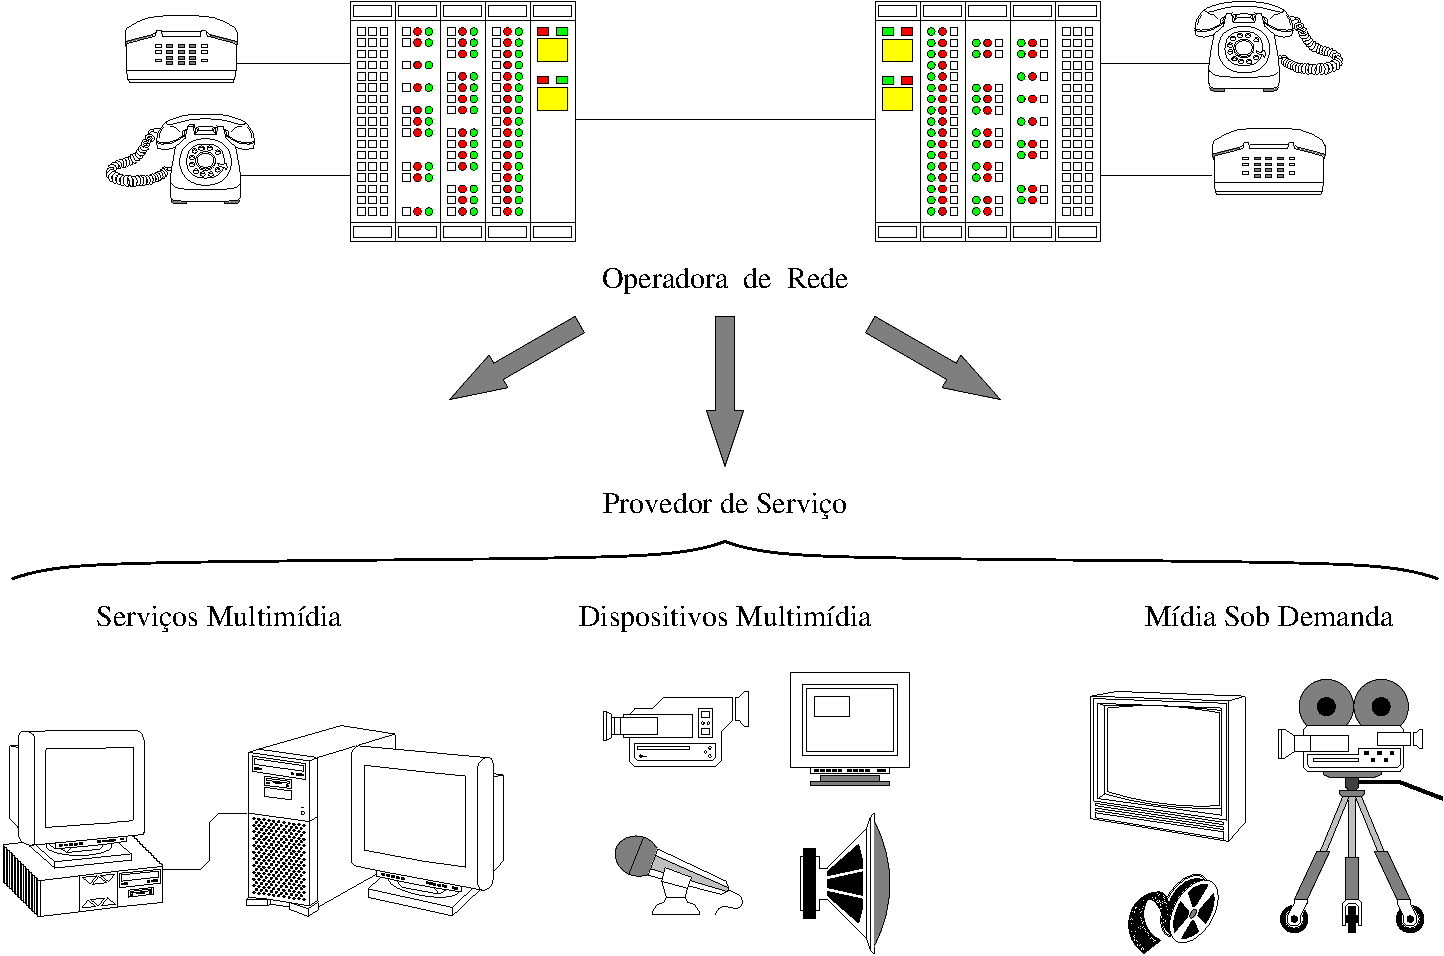
\includegraphics[width=0.55\textwidth]{./CapituloExemplo/figura1}%% Dimensões e localização
\fonte{\citet{Larsson2003}.}%% Fonte
\end{figure}

Figuras em formato GIF, JPEG e BMP podem ser convertidas para o formato \gls{eps} através do aplicativo ``xv''. O ``xv'' não lista o formato \gls{eps} dentre aqueles que é capaz de manipular. Entretanto, selecionando-se o formato \textit{PostScript} e fornecendo-se a extensão \texttt{eps} ao nome do arquivo, o formato \gls{eps} é gerado.

O ambiente \texttt{picture} permite a programação de imagens diretamente no \gls{latex}\index{LaTeX@\latex}, conforme exemplo apresentado na \autoref{fig:figura2}.

\begin{figure}[htb]%% Ambiente figure
\captionsetup{width=8cm}%% Largura da legenda
\caption{Exemplo de figura criada a partir do ambiente \texttt{picture}.}%% Legenda
\label{fig:figura2}%% Rótulo
\setlength{\unitlength}{1cm}%% Unidade de comprimento
\begin{picture}(8,5)(-4,-2.5)%% Ambiente picture
\put(-4,0){\vector(1,0){8}}
\put(3.75,-0.25){$\chi$}
\put(0,-2.5){\vector(0,1){5}}
\multiput(-4,1)(0.4,0){20}{\line(1,0){0.2}}
\multiput(-4,-1)(0.4,0){20}{\line(1,0){0.2}}
\put(0.25,2.25){$\beta \equiv v / c = \tanh \chi$}
\qbezier(0,0)(0.8853,0.8853)(2,0.9640)
\qbezier(0,0)(-0.8853,-0.8853)(-2,-0.9640)
\end{picture}
\fonte{Autoria própria.}%% Fonte
\end{figure}

A \autoref{fig:subfigure} apresenta um exemplo usando o pacote \texttt{subfigure} com legendas usando o pacote \texttt{subcaption}. É  possível referenciar cada uma das sub-figuras, no qual, a sua referência alfabética aparece entre parênteses: \autoref{fig:subfigure_a} e \autoref{fig:subfigure_b}.

\begin{figure}[!ht]
\centering
\caption{Exemplo de Subfigure} 
\label{fig:subfigure}
\begin{subfigure}[t]{.45\textwidth}
	\centering
	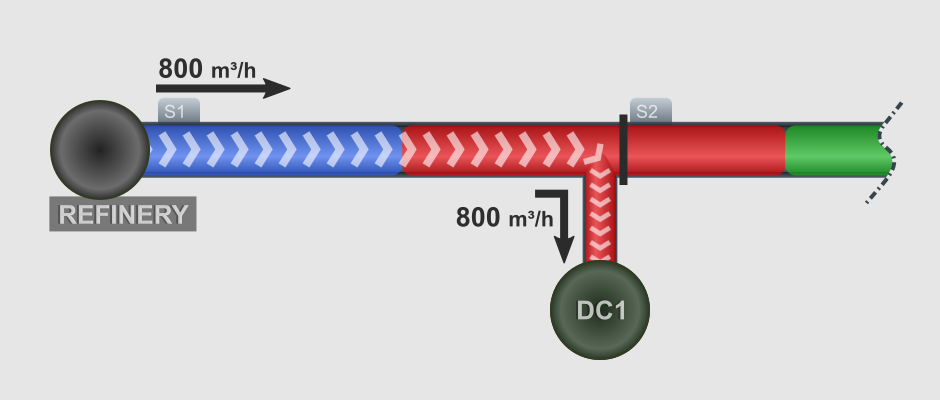
\includegraphics[width=\textwidth]{./CapituloExemplo/subfigure-a.png}
	\caption{Figura A}
	\label{fig:subfigure_a}
\end{subfigure}
\qquad
\begin{subfigure}[t]{.45\textwidth}
	\centering
	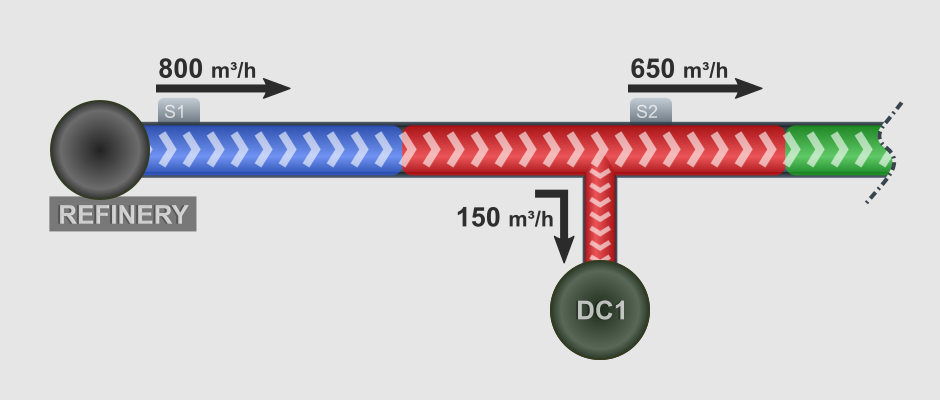
\includegraphics[width=\textwidth]{./CapituloExemplo/subfigure-b.png}  
	\caption{Figura B}
	\label{fig:subfigure_b}
\end{subfigure}
\fonte{\citet{Meira2020}} %citeonline{meira2020}
\end{figure}

%% Título e rótulo de seção (rótulos não devem conter caracteres especiais, acentuados ou cedilha)
\subsection{Fotografias}\label{sec:fotografias}

Um exemplo deste tipo de ilustração é apresentado na \autoref{foto:foto1}.

\begin{photograph}[htb]%% Ambiente photograph
\captionsetup{width=0.6\textwidth}%% Largura da legenda
\caption{Camaleão pantera fotografado por Joel Sartore, National Geographic.}%% Legenda
\label{foto:foto1}%% Rótulo
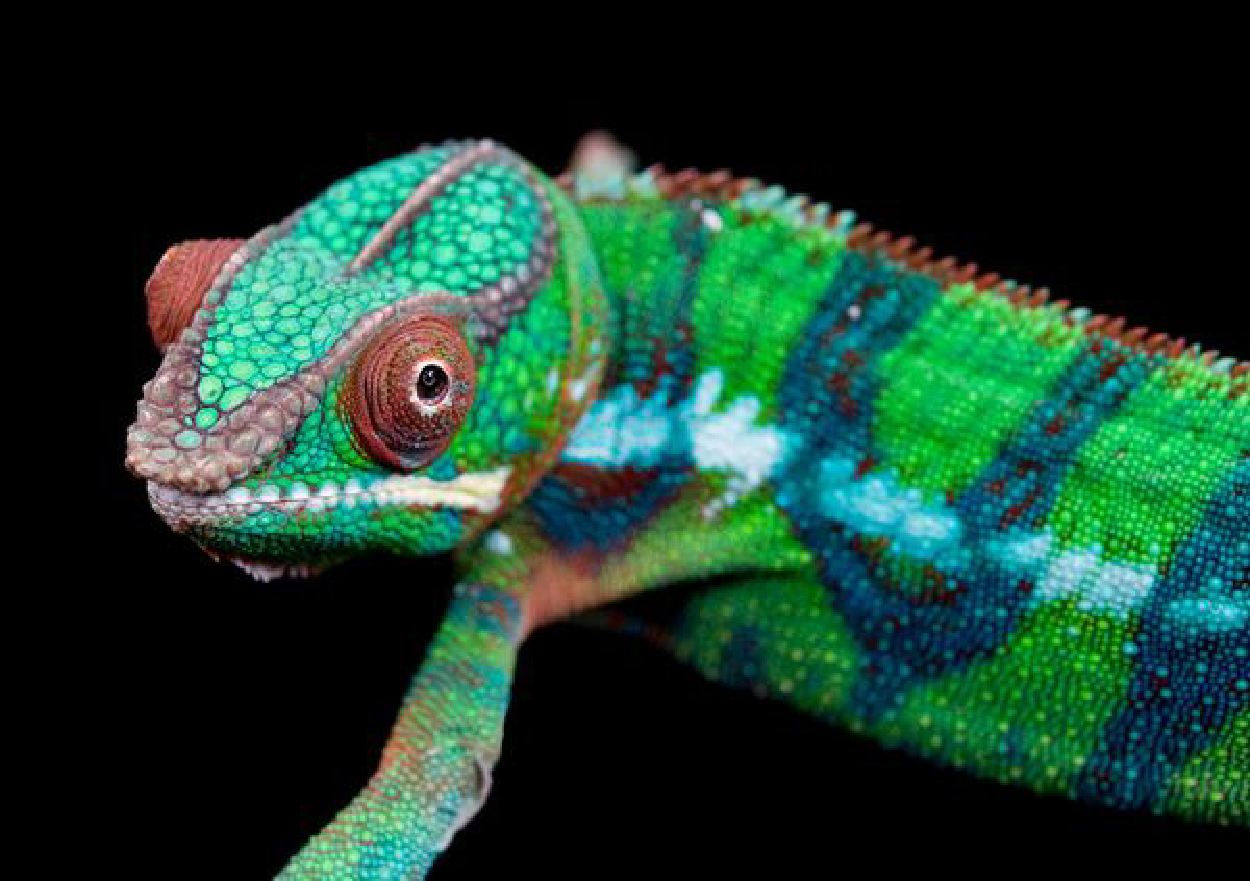
\includegraphics[width=0.6\textwidth]{./CapituloExemplo/foto1}%% Dimensões e localização
\fonte{\citet{Sartore2013}.}%% Fonte
\end{photograph}

Outro exemplo deste tipo de ilustração é apresentado na \autoref{foto:foto2}.

\begin{photograph}[htb]%% Ambiente photograph
\captionsetup{width=0.6\textwidth}%% Largura da legenda
\caption{Fotografia da erupção vulcânica em 1982 do Galungung, Indonésia (com descargas de raios), produzida pelo Serviço Geológico dos Estados Unidos da América.}%% Legenda
\label{foto:foto2}%% Rótulo
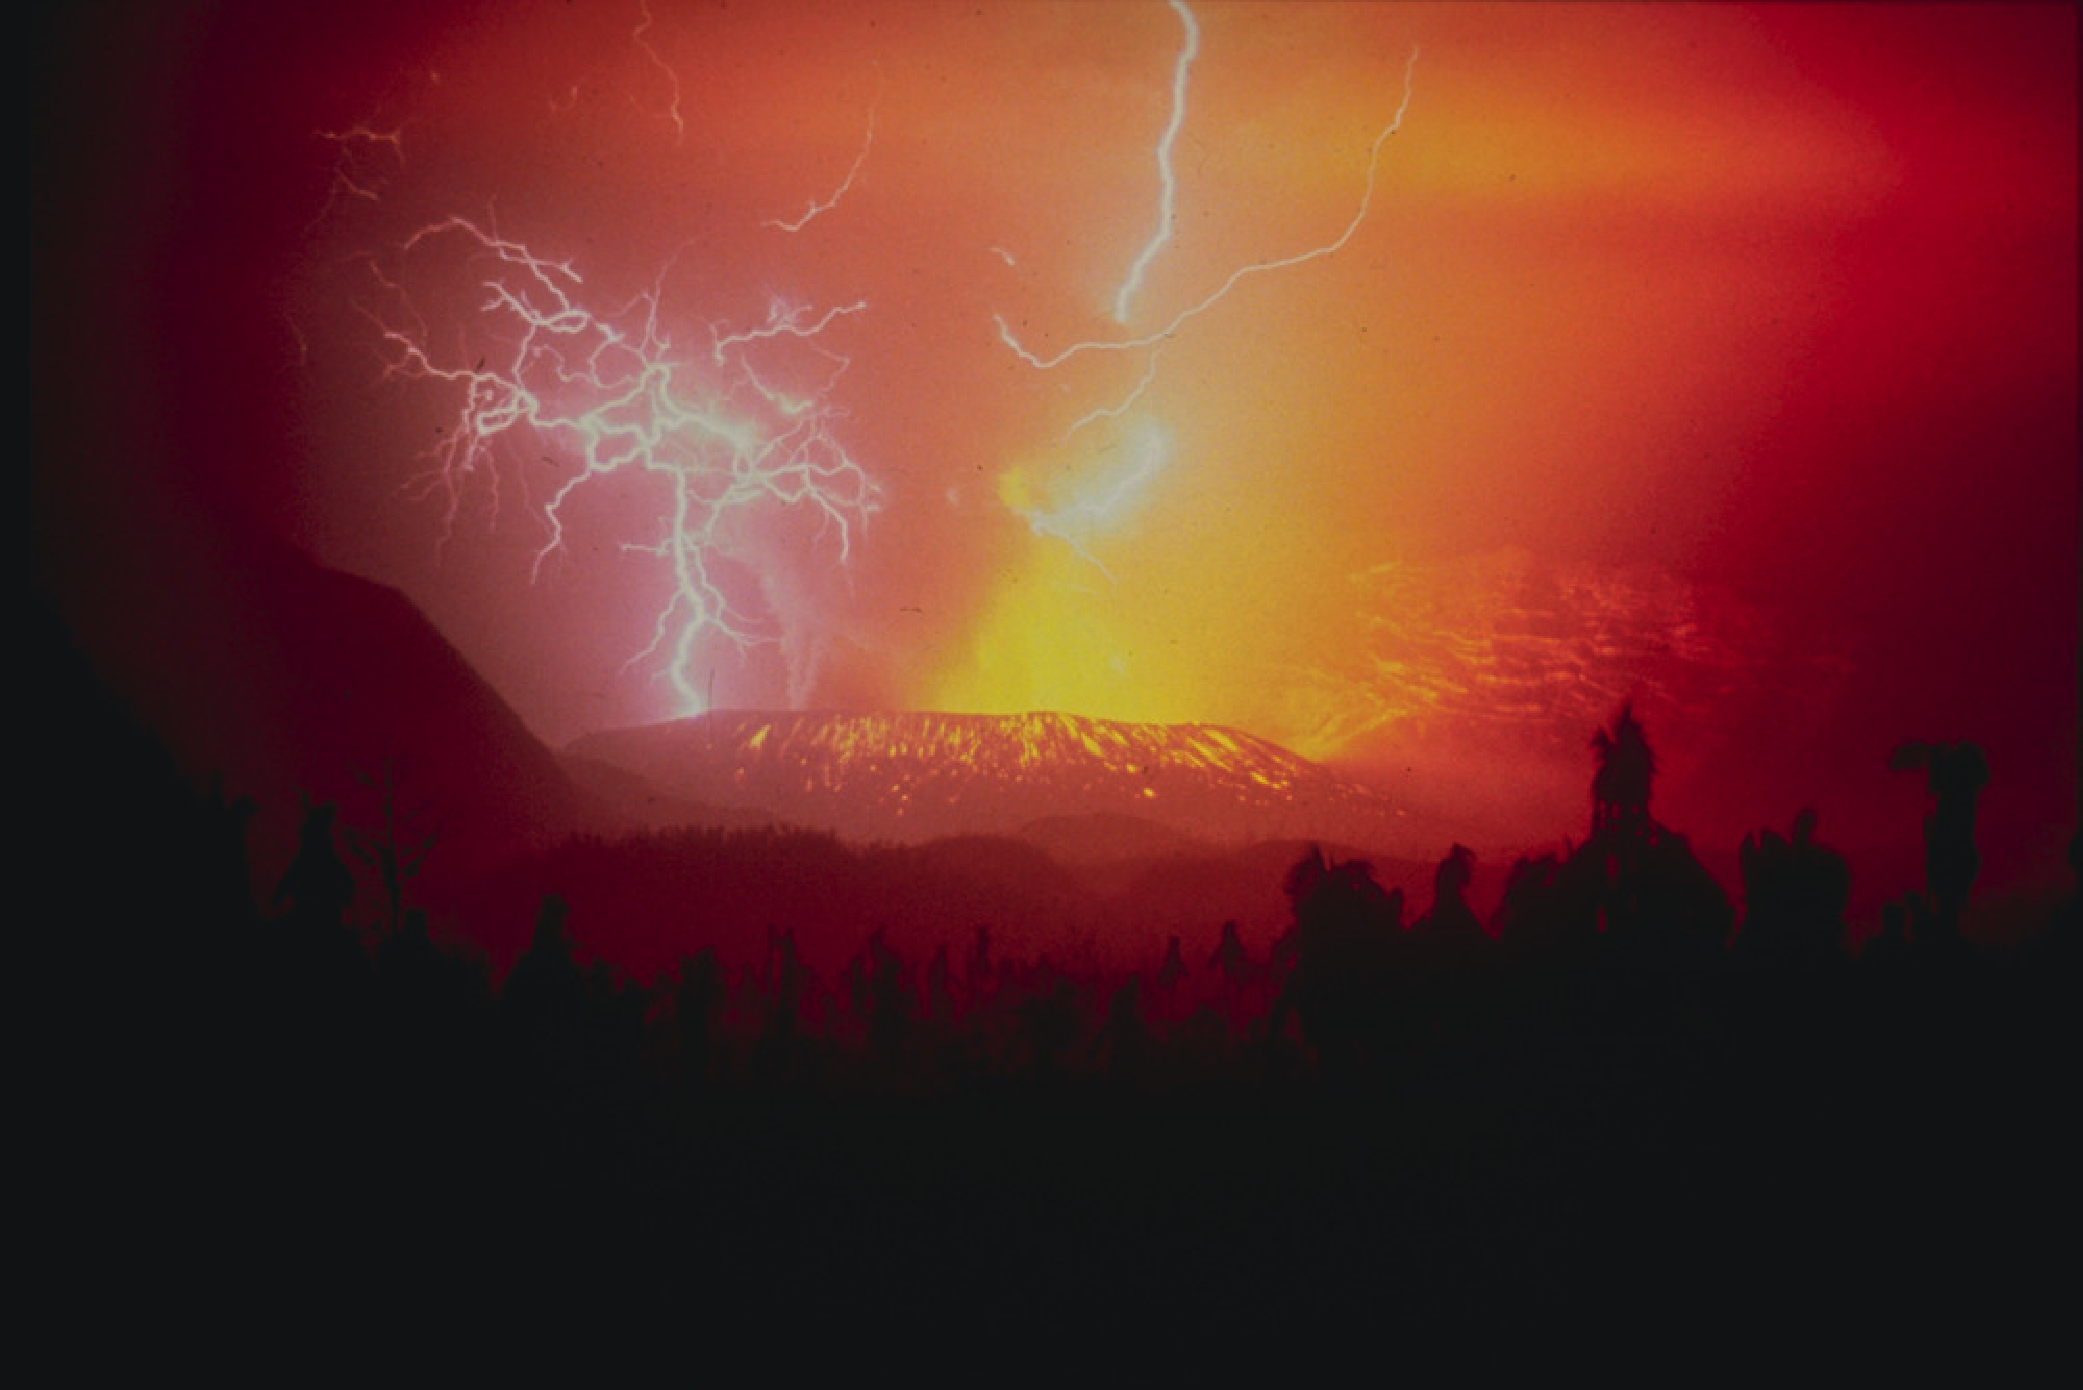
\includegraphics[width=0.6\textwidth]{./CapituloExemplo/foto2}%% Dimensões e localização
\fonte{\citet{Hadian1982}.}%% Fonte
\end{photograph}

%% Título e rótulo de seção (rótulos não devem conter caracteres especiais, acentuados ou cedilha)
\subsection{Gráficos}\label{sec:graficos}

Gráficos são gerados com aplicativos capazes de exportar nos formatos \gls{ps} ou \gls{eps}. A ferramenta ``gnuplot'' é uma das mais utilizadas para a geração de gráficos (\url{http://www.gnuplot.info/}). Uma vez no formato \gls{eps}, gráficos são inseridos no texto tal como figuras (veja \autoref{gra:grafico1}).

\begin{graph}[htb]%% Ambiente graph
\captionsetup{width=0.6\textwidth}%% Largura da legenda
\caption{Exemplo de gráfico produzido em ``gnuplot''.}%% Legenda
\label{gra:grafico1}%% Rótulo
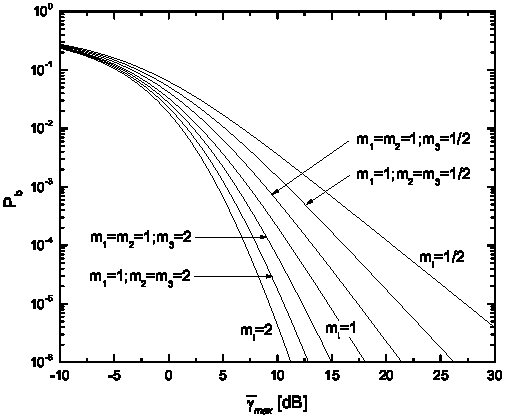
\includegraphics[width=0.6\textwidth]{./CapituloExemplo/grafico1}%% Dimensões e localização
\fonte{\citet{Faina2001}.}%% Fonte
\end{graph}

No \autoref{gra:grafico2} é apresentado um exemplo de gráfico produzido em ``Excel''.

\begin{graph}[htb]%% Ambiente graph
\captionsetup{width=0.6\textwidth}%% Largura da legenda
\caption{Exemplo de gráfico produzido em ``Excel''.}%% Legenda
\label{gra:grafico2}%% Rótulo
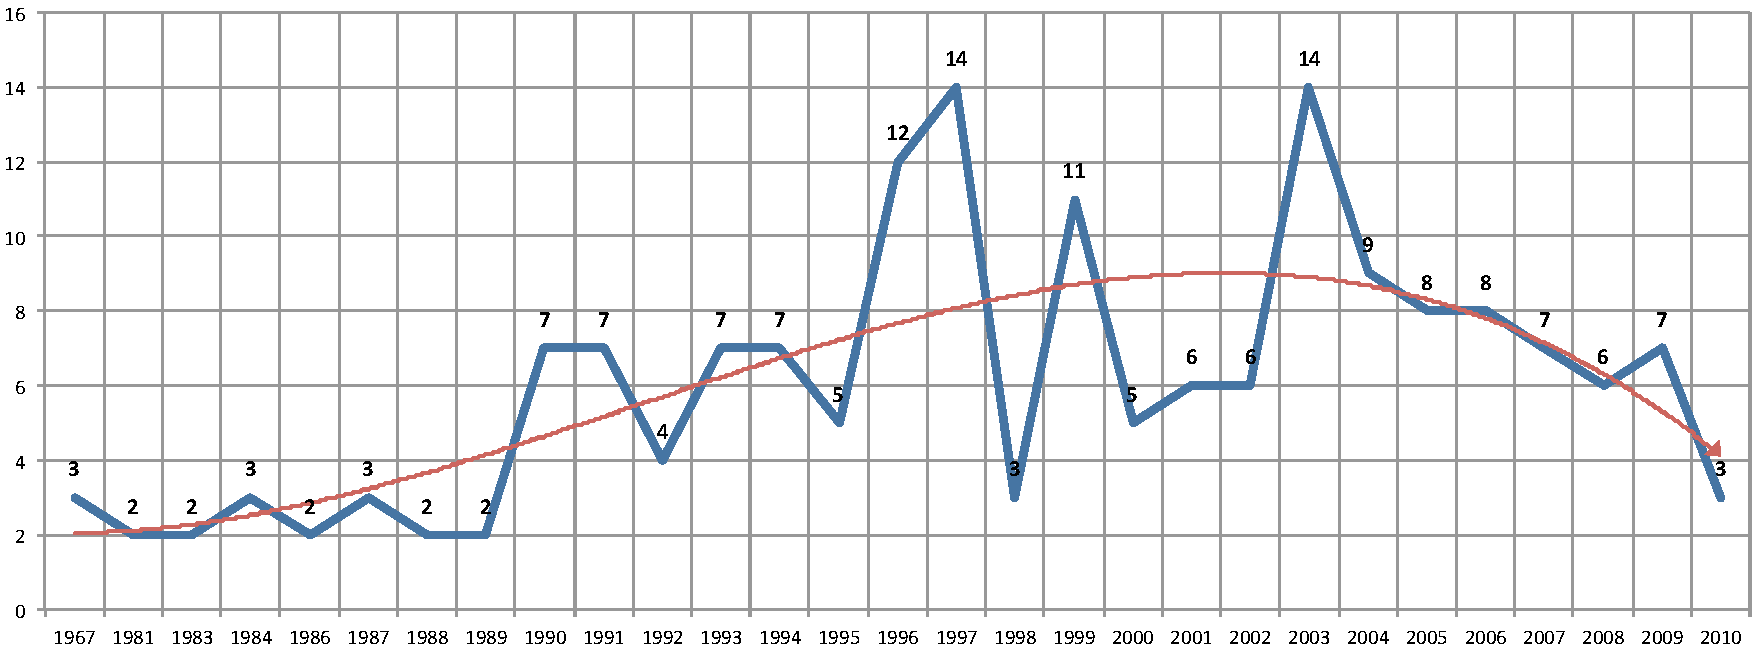
\includegraphics[width=0.6\textwidth]{./CapituloExemplo/grafico2}%% Dimensões e localização
\fonte{\citeonline[p. 24]{Araujo2012}.}%% Fonte
\end{graph}

O ambiente \texttt{minipage} pode ser usado para inserir textos ou outros elementos em quadros com tamanhos e posições controladas, conforme exemplos apresentados no \autoref{gra:minipagegrafico1} e no \autoref{gra:minipagegrafico2}.

\begin{graph}[htb]%% Ambiente graph
\begin{minipage}[t]{0.395\textwidth}%% Ambiente minipage
\centering%% Centralizado
\captionsetup{width=0.85\textwidth}%% Largura da legenda
\caption{Gráfico 1 do ambiente \texttt{minipage}.}%% Legenda
\label{gra:minipagegrafico1}%% Rótulo
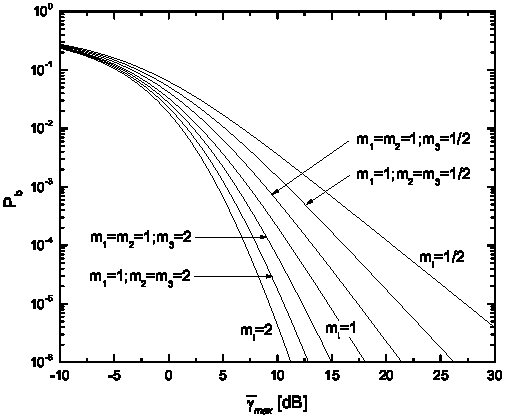
\includegraphics[width=0.85\textwidth]{./CapituloExemplo/grafico1}%% Dimensões e localização
\fonte{\citet{Faina2001}.}%% Fonte
\end{minipage}
\hfill
\begin{minipage}[t]{0.595\textwidth}%% Ambiente minipage
\centering%% Centralizado
\captionsetup{width=0.95\textwidth}%% Largura da legenda
\caption{Gráfico 2 do ambiente \texttt{minipage}.}%% Legenda
\label{gra:minipagegrafico2}%% Rótulo
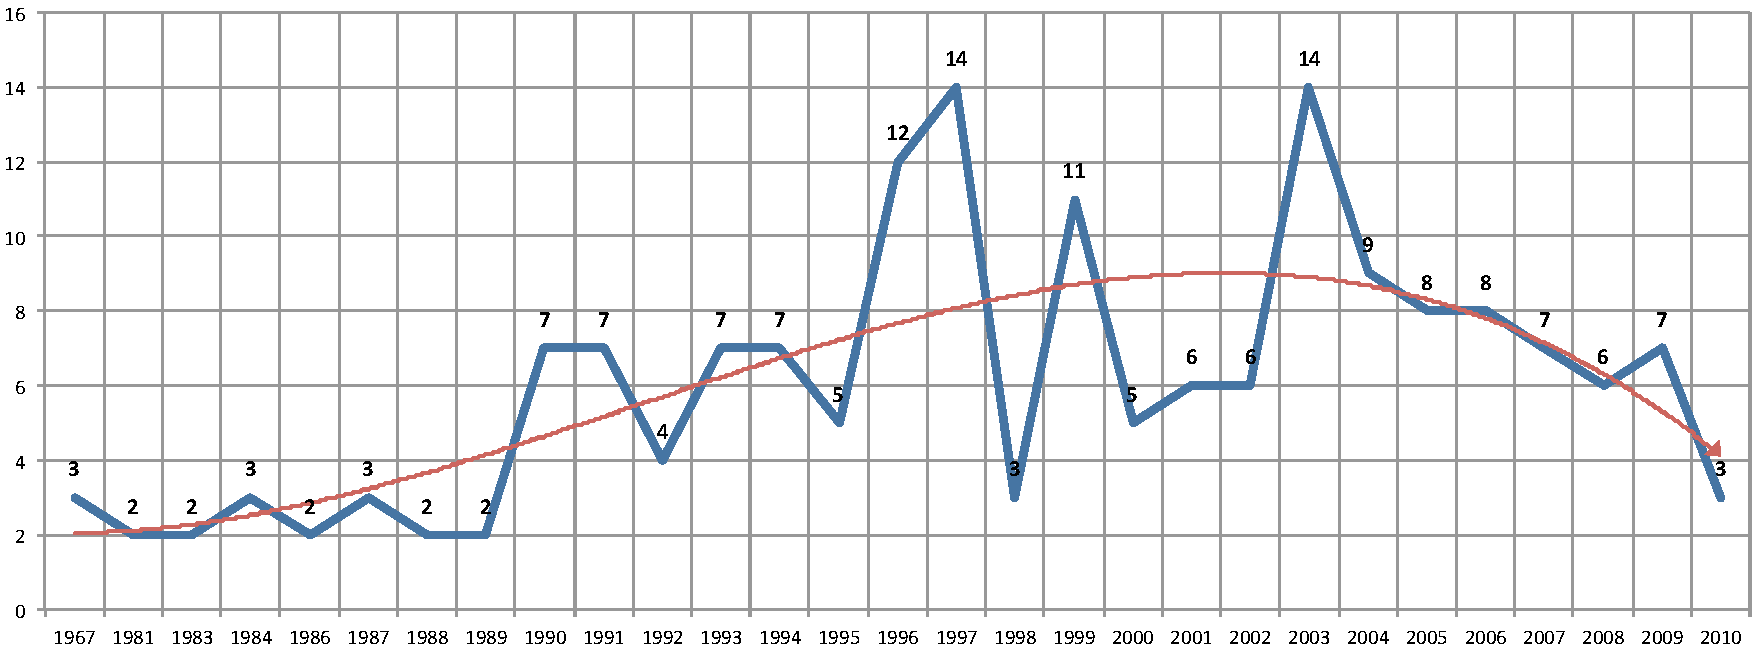
\includegraphics[width=0.95\textwidth]{./CapituloExemplo/grafico2}%% Dimensões e localização
\fonte{\citeonline[p. 24]{Araujo2012}}%% Fonte
\end{minipage}
\label{gra:minipagegraficos}
\end{graph}

%% Título e rótulo de seção (rótulos não devem conter caracteres especiais, acentuados ou cedilha)
\subsection{Quadros}\label{sec:quadros}

Um exemplo deste tipo de ilustração é apresentado no \autoref{quad:quadro1}.

\begin{tabframed}[htb]%% Ambiente tabframed
\captionsetup{width=0.5\textwidth}%% Largura da legenda
\caption{Compostos orgânicos: fórmulas estruturais e principais classes.}%% Legenda
\label{quad:quadro1}%% Rótulo
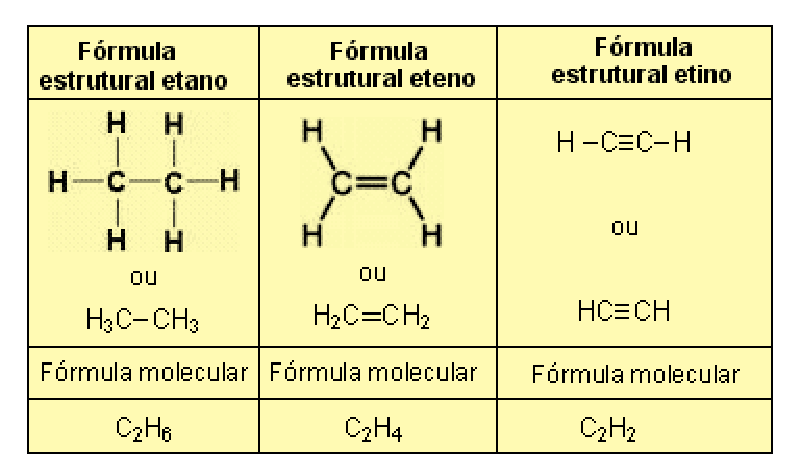
\includegraphics[width=0.5\textwidth]{./CapituloExemplo/quadro1}%% Dimensões e localização
\fonte{\citet{daSilva2009}.}%% Fonte
\end{tabframed}

Outro exemplo deste tipo de ilustração é apresentado no \autoref{quad:quadro2}.

\begin{tabframed}[htb]%% Ambiente tabframed
\captionsetup{width=0.7\textwidth}%% Largura da legenda
\caption{Modelos de maturidade para a gestão da cadeia de suprimentos.}%% Legenda
\label{quad:quadro2}%% Rótulo
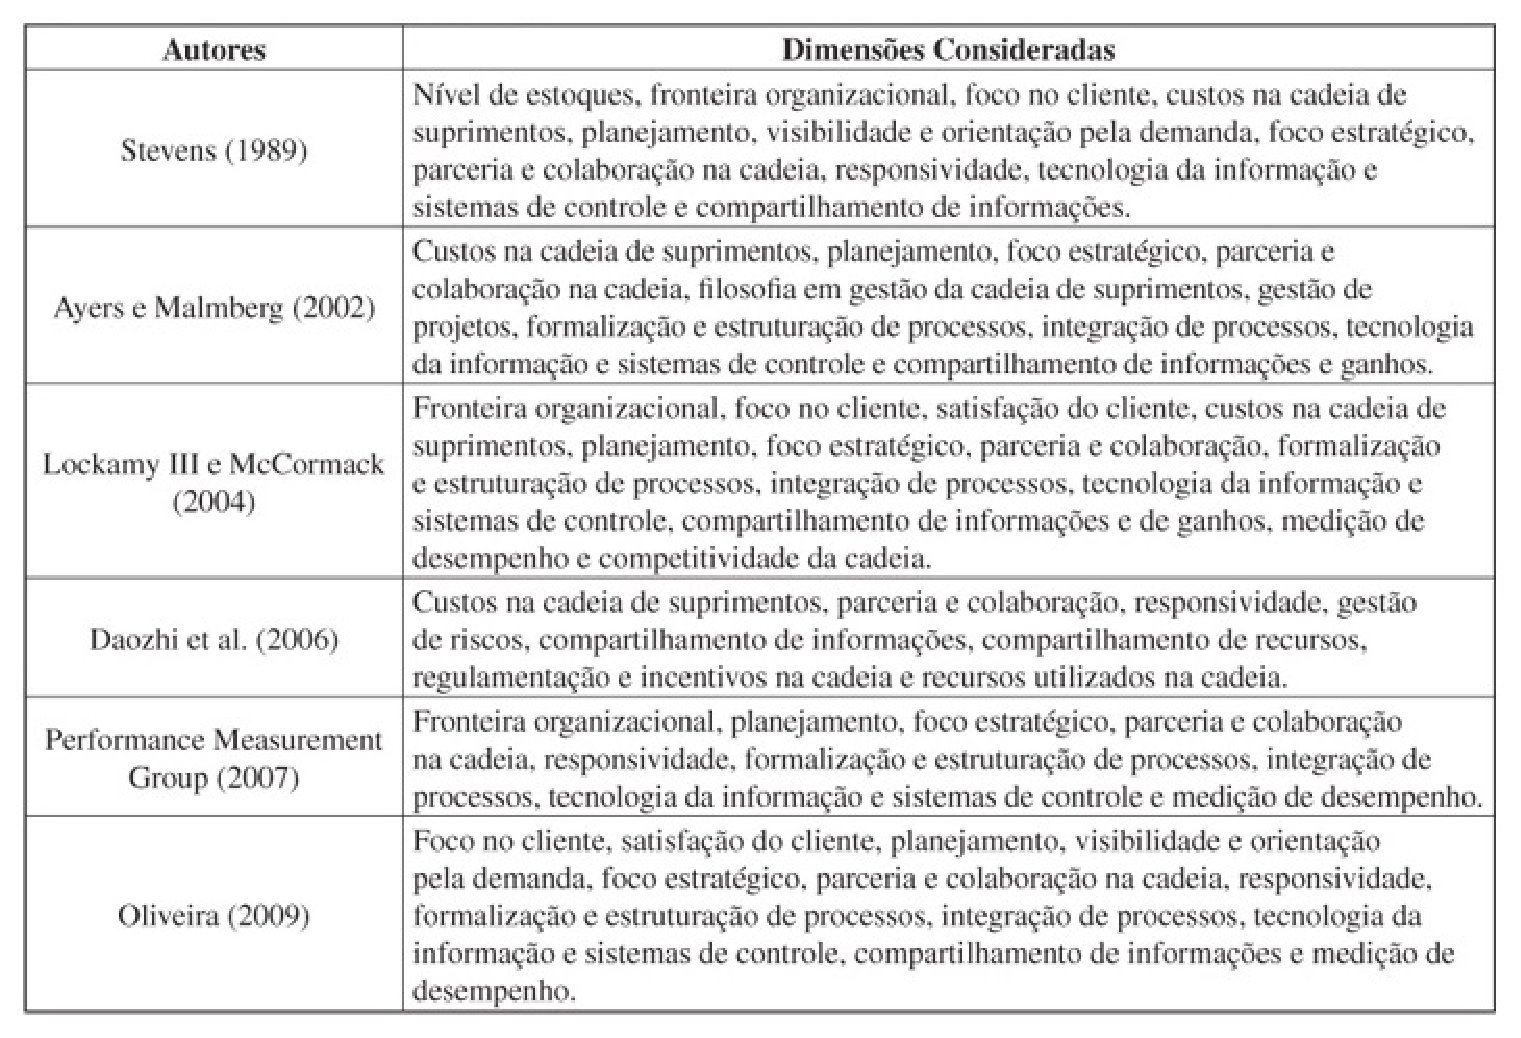
\includegraphics[width=0.7\textwidth]{./CapituloExemplo/quadro2}%% Dimensões e localização
\fonte{\citet{Frederico2012}.}%% Fonte
\end{tabframed}

Os quadros não devem ser chamados de tabelas, uma vez que se diferenciam destas por apresentarem as laterais fechadas e o conteúdo não numérico.

%% Título e rótulo de seção (rótulos não devem conter caracteres especiais, acentuados ou cedilha)
\section{Tabelas}\label{sec:tabelas}

Tabelas são construídas com comandos próprios do \gls{latex}\index{LaTeX@\latex}. Por exemplo, a \autoref{tab:tabela1} foi construída desta forma.

\begin{table}[htb]%% Ambiente table
\caption{Primeiro exemplo de tabela com uma legenda contendo um texto muito longo que pode ocupar mais de uma linha.}%% Legenda
\label{tab:tabela1}%% Rótulo
\begin{tabularx}{\textwidth}{@{\extracolsep{\fill}}llll}%% Ambiente tabularx
\toprule
$\bsym{L}$ & $\bsym{L^2}$ & $\bsym{L^3}$ & $\bsym{L^4}$ \\
\SI{}{[m]} & \SI{}{[m^2]} & \SI{}{[m^3]} & \SI{}{[m^4]} \\ \midrule
1          & 1            & 1            & 1            \\
2          & 4            & 8            & 16           \\
3          & 9            & 27           & 81           \\
4          & 16           & 64           & 256          \\
5          & 25           & 125          & 625          \\ \bottomrule
\end{tabularx}
\fonte{Autoria própria.}%% Fonte
\end{table}

A \autoref{tab:tabela2} é um exemplo de tabela que ocupa mais de uma página e que foi construída pelo \gls{latex}\index{LaTeX@\latex} utilizando o pacote \texttt{longtable}.

\begin{longtable}{@{\extracolsep{\fill}}lll}%% Ambiente longtable
\caption{Possíveis tríplices para grade altamente variável.\label{tab:tabela2}} \\%% Legenda e rótulo
\toprule
\textbf{Tempo (s)} & \textbf{Tríplice escolhida} & \textbf{Outras possíveis tríplices} \\
\midrule
\endfirsthead%% Encerra cabeçalho da primeira página
\caption[]{Possíveis tríplices para grade altamente variável.} \\%% Legenda
\multicolumn{3}{r}{\textbf{(continuação)}} \\
\toprule
\textbf{Tempo (s)} & \textbf{Tríplice escolhida} & \textbf{Outras possíveis tríplices} \\
\midrule
\endhead%% Encerra cabeçalho das demais páginas
\midrule
\multicolumn{3}{r}{\textbf{(continua)}} \\
\endfoot%% Encerra rodapé das demais páginas
\bottomrule
\\[-0.5\linha]
\caption*{\nomefonte: Adaptado de \citet{Smallen2014}.} \\
\endlastfoot%% Encerra rodapé da última página
0      & (1, 11, 13725) & (1, 12, 10980), (1, 13, 8235), (2, 2, 0), (3, 1, 0) \\
2745   & (1, 12, 10980) & (1, 13, 8235), (2, 2, 0), (2, 3, 0), (3, 1, 0)      \\
5490   & (1, 12, 13725) & (2, 2, 2745), (2, 3, 0), (3, 1, 0)                  \\
8235   & (1, 12, 16470) & (1, 13, 13725), (2, 2, 2745), (2, 3, 0), (3, 1, 0)  \\
10980  & (1, 12, 16470) & (1, 13, 13725), (2, 2, 2745), (2, 3, 0), (3, 1, 0)  \\
13725  & (1, 12, 16470) & (1, 13, 13725), (2, 2, 2745), (2, 3, 0), (3, 1, 0)  \\
16470  & (1, 13, 16470) & (2, 2, 2745), (2, 3, 0), (3, 1, 0)                  \\
19215  & (1, 12, 16470) & (1, 13, 13725), (2, 2, 2745), (2, 3, 0), (3, 1, 0)  \\
21960  & (1, 12, 16470) & (1, 13, 13725), (2, 2, 2745), (2, 3, 0), (3, 1, 0)  \\
24705  & (1, 12, 16470) & (1, 13, 13725), (2, 2, 2745), (2, 3, 0), (3, 1, 0)  \\
27450  & (1, 12, 16470) & (1, 13, 13725), (2, 2, 2745), (2, 3, 0), (3, 1, 0)  \\
30195  & (2, 2, 2745)   & (2, 3, 0), (3, 1, 0)                                \\
32940  & (1, 13, 16470) & (2, 2, 2745), (2, 3, 0), (3, 1, 0)                  \\
35685  & (1, 13, 13725) & (2, 2, 2745), (2, 3, 0), (3, 1, 0)                  \\
38430  & (1, 13, 10980) & (2, 2, 2745), (2, 3, 0), (3, 1, 0)                  \\
41175  & (1, 12, 13725) & (1, 13, 10980), (2, 2, 2745), (2, 3, 0), (3, 1, 0)  \\
43920  & (1, 13, 10980) & (2, 2, 2745), (2, 3, 0), (3, 1, 0)                  \\
46665  & (2, 2, 2745)   & (2, 3, 0), (3, 1, 0)                                \\
49410  & (2, 2, 2745)   & (2, 3, 0), (3, 1, 0)                                \\
52155  & (1, 12, 16470) & (1, 13, 13725), (2, 2, 2745), (2, 3, 0), (3, 1, 0)  \\
54900  & (1, 13, 13725) & (2, 2, 2745), (2, 3, 0), (3, 1, 0)                  \\
57645  & (1, 13, 13725) & (2, 2, 2745), (2, 3, 0), (3, 1, 0)                  \\
60390  & (1, 12, 13725) & (2, 2, 2745), (2, 3, 0), (3, 1, 0)                  \\
63135  & (1, 13, 16470) & (2, 2, 2745), (2, 3, 0), (3, 1, 0)                  \\
65880  & (1, 13, 16470) & (2, 2, 2745), (2, 3, 0), (3, 1, 0)                  \\
68625  & (2, 2, 2745)   & (2, 3, 0), (3, 1, 0)                                \\
71370  & (1, 13, 13725) & (2, 2, 2745), (2, 3, 0), (3, 1, 0)                  \\
74115  & (1, 12, 13725) & (2, 2, 2745), (2, 3, 0), (3, 1, 0)                  \\
76860  & (1, 13, 13725) & (2, 2, 2745), (2, 3, 0), (3, 1, 0)                  \\
79605  & (1, 13, 13725) & (2, 2, 2745), (2, 3, 0), (3, 1, 0)                  \\
82350  & (1, 12, 13725) & (2, 2, 2745), (2, 3, 0), (3, 1, 0)                  \\
85095  & (1, 12, 13725) & (1, 13, 10980), (2, 2, 2745), (2, 3, 0), (3, 1, 0)  \\
87840  & (1, 13, 16470) & (2, 2, 2745), (2, 3, 0), (3, 1, 0)                  \\
90585  & (1, 13, 16470) & (2, 2, 2745), (2, 3, 0), (3, 1, 0)                  \\
93330  & (1, 13, 13725) & (2, 2, 2745), (2, 3, 0), (3, 1, 0)                  \\
96075  & (1, 13, 16470) & (2, 2, 2745), (2, 3, 0), (3, 1, 0)                  \\
98820  & (1, 13, 16470) & (2, 2, 2745), (2, 3, 0), (3, 1, 0)                  \\
101565 & (1, 13, 13725) & (2, 2, 2745), (2, 3, 0), (3, 1, 0)                  \\
104310 & (1, 13, 16470) & (2, 2, 2745), (2, 3, 0), (3, 1, 0)                  \\
107055 & (1, 13, 13725) & (2, 2, 2745), (2, 3, 0), (3, 1, 0)                  \\
109800 & (1, 13, 13725) & (2, 2, 2745), (2, 3, 0), (3, 1, 0)                  \\
112545 & (1, 12, 16470) & (1, 13, 13725), (2, 2, 2745), (2, 3, 0), (3, 1, 0)  \\
115290 & (1, 13, 16470) & (2, 2, 2745), (2, 3, 0), (3, 1, 0)                  \\
118035 & (1, 13, 13725) & (2, 2, 2745), (2, 3, 0), (3, 1, 0)                  \\
120780 & (1, 13, 16470) & (2, 2, 2745), (2, 3, 0), (3, 1, 0)                  \\
123525 & (1, 13, 13725) & (2, 2, 2745), (2, 3, 0), (3, 1, 0)                  \\
126270 & (1, 12, 16470) & (1, 13, 13725), (2, 2, 2745), (2, 3, 0), (3, 1, 0)  \\
129015 & (2, 2, 2745)   & (2, 3, 0), (3, 1, 0)                                \\
131760 & (2, 2, 2745)   & (2, 3, 0), (3, 1, 0)                                \\
134505 & (1, 13, 16470) & (2, 2, 2745), (2, 3, 0), (3, 1, 0)                  \\
137250 & (1, 13, 13725) & (2, 2, 2745), (2, 3, 0), (3, 1, 0)                  \\
139995 & (2, 2, 2745)   & (2, 3, 0), (3, 1, 0)                                \\
142740 & (2, 2, 2745)   & (2, 3, 0), (3, 1, 0)                                \\
145485 & (1, 12, 16470) & (1, 13, 13725), (2, 2, 2745), (2, 3, 0), (3, 1, 0)  \\
148230 & (2, 2, 2745)   & (2, 3, 0), (3, 1, 0)                                \\
150975 & (1, 13, 16470) & (2, 2, 2745), (2, 3, 0), (3, 1, 0)                  \\
153720 & (1, 12, 13725) & (2, 2, 2745), (2, 3, 0), (3, 1, 0)                  \\
156465 & (1, 13, 13725) & (2, 2, 2745), (2, 3, 0), (3, 1, 0)                  \\
159210 & (1, 13, 13725) & (2, 2, 2745), (2, 3, 0), (3, 1, 0)                  \\
161955 & (1, 13, 16470) & (2, 2, 2745), (2, 3, 0), (3, 1, 0)                  \\
164700 & (1, 13, 13725) & (2, 2, 2745), (2, 3, 0), (3, 1, 0)                  \\
\end{longtable}

Tabelas criadas em planilhas do ``Excel'' podem ser convertidas em tabelas \gls{latex}\index{LaTeX@\latex} através do suplemento ``Excel-to-LaTeX'', disponível em \url{http://www.ctan.org/pkg/excel2latex}.

%% Título e rótulo de seção (rótulos não devem conter caracteres especiais, acentuados ou cedilha)
\section{Abreviaturas, Siglas e Acrônimos}\label{sec:acronimos}

\gls{latex}\index{LaTeX@\latex} gera automaticamente a lista de abreviaturas, siglas e acrônimos através do pacote \texttt{glossaries}. As abreviaturas, siglas e acrônimos devem ser definidos no arquivo \texttt{entradas-acronimos.tex}, no diretório ``PreTexto'', com os comandos:

\begin{SingleSpacing}%% Ambiente SingleSpacing
\begin{verbatim}
\abreviatura{rótulo}{representação}{definição}
\sigla{rótulo}{representação}{definição}
\acronimo{rótulo}{representação}{definição}
\end{verbatim}
\end{SingleSpacing}

Para que a abreviatura, sigla ou acrônimo seja apresentada em alguma parte do texto do documento use o comando \verb|\gls{rótulo}|, por exemplo, as abreviaturas \gls{art.}, \gls{cap.} e \gls{sec.} foram geradas pelos comandos \verb|\gls{art.}, \gls{cap.} e \gls{sec.}|, respectivamente. Mais detalhes dos comandos do pacote \texttt{glossaries} podem ser encontrados em: \url{http://mirrors.ctan.org/macros/latex/contrib/glossaries/glossaries-user.pdf}.

Outra opção para gerar a lista de abreviaturas, siglas e acrônimos é através da edição manual do arquivo \texttt{lista-acronimos.tex} no diretório ``PreTexto''.

%% Título e rótulo de seção (rótulos não devem conter caracteres especiais, acentuados ou cedilha)
\section{Símbolos}\label{sec:simbolos}

\gls{latex}\index{LaTeX@\latex} gera automaticamente a lista de símbolos através do pacote \texttt{nomencl}. Ao redigir um símbolo pela primeira vez em qualquer parte do texto com o comando \verb|\nomenclature[prefixo]{símbolo}{descrição \nomunit{unidade}}|, é gerada uma entrada para a lista de símbolos. Veja exemplos deste comando no arquivo fonte deste capítulo. Os elementos da lista de símbolos são ordenados a depender da primeira letra atribuída ao prefixo e classificadas em:

\begin{itemize}%% Lista de itens
\item A~-~Letras Latinas.
\item B~-~Letras Gregas.
\item C~-~Sobrescritos.
\item D~-~Subscritos.
\item E~-~Notações.
\item F~-~Índices e Conjuntos
\item G~-~Parâmetros
\item H~-~Variáveis contínuas
\item I~-~Variáveis inteiras
\item J~-~Variáveis binárias
\end{itemize}

Outra opção ao comando \verb|\nomenclature| é o uso dos atalhos:

\begin{SingleSpacing}%% Ambiente SingleSpacing
\begin{verbatim}
\letralatina{prefixo}{símbolo}{descrição}{unidade}
\letragrega{prefixo}{símbolo}{descrição}{unidade}
\sobrescrito{prefixo}{símbolo}{descrição}{unidade}
\subscrito{prefixo}{símbolo}{descrição}{unidade}
\notacao{prefixo}{símbolo}{descrição}{unidade}
\notacaois{símbolo}{descrição}{unidade}
\notacaoparam{símbolo}{descrição}{unidade}
\notacaofloatvar{símbolo}{descrição}{unidade}
\notacaointvar{símbolo}{descrição}{unidade}
\notacaobinvar{símbolo}{descrição}{unidade}
\end{verbatim}
\end{SingleSpacing}

\noindent Neste caso a atribuição da primeira letra do prefixo pode ser desprezada.

%% Letras Latinas [A]
\nomenclature[AA]{$A$}{Área \nomunit{m^2}}%%
\letralatina{L}{L}{Comprimento}{m}%%
\letralatina{R}{R}{Raio}{m}%%
%% Letras Gregas [B]
\nomenclature[Bmu]{$\mu$}{Viscosidade dinâmica \nomunit{kg/(m.s)}}%%
\letragrega{nu}{\nu}{Viscosidade cinemática}{m^2/s}%%
\letragrega{pi}{\pi}{Pi (constante circular)}{rad}%%
\letragrega{rho}{\rho}{Massa específica}{kg/m^3}%%
\letragrega{sigma}{\sigma}{Tensão superficial}{N/m}%%
%% Sobrescritos [C]
\nomenclature[C+]{$+$}{Passo de tempo posterior}%%
\sobrescrito{-}{-}{Passo de tempo anterior}{}%%
\sobrescrito{0}{0}{Valor inicial}{}%%
%% Subscritos [D]
\nomenclature[DG]{$G$}{Fase gasosa}%%
\subscrito{L}{L}{Fase líquida}{}%%
\subscrito{S}{S}{Fase sólida}{}%%
%% Notações [E]
\nomenclature[EPsi_1]{$\overline{\Psi}$}{Média temporal}%%
\notacao{Psi_2}{\langle \Psi \rangle}{Média na seção transversal}{}%%
\notacao{Psi_3}{\langle\langle \Psi \rangle\rangle}{Média na seção transversal ponderada}{}%%
%% Notações [F]
\notacaois{Event_set}{e \in E}{Set of events}{}
\notacaois{Interval_set}{i \in I}{Set of intervals}{}
%% Notações [H]
\notacaoparam{eps}{\varepsilon}{Small constant value}{}
\notacaoparam{lb}{L}{Lower bound value ($L \ll 0$)}{}
%% Notações [I]
\notacaofloatvar{end}{e_{i}}{End of interval $i$}{h}
\notacaofloatvar{start}{s_{i}}{Start of interval $i$}{h}
%% Notações [J]
\notacaointvar{e_i}{\phi_i}{Number of employees set to work during interval $i$}{}
%% Notações [K]
\notacaobinvar{a_i}{a_{i}}{1 if the flow is active during interval $i$; 0 otherwise}{}

Mais detalhes dos comandos do pacote \texttt{nomencl} podem ser encontrados em: \url{http://tug.ctan.org/tex-archive/macros/latex/contrib/nomencl/nomencl.pdf}.

Outra opção para gerar a lista de símbolos é através da edição manual do arquivo \texttt{lista-simbolos.tex} no diretório ``PreTexto''.

%% Título e rótulo de seção (rótulos não devem conter caracteres especiais, acentuados ou cedilha)
\section{Inclusão de Outros Arquivos}\label{sec:inclusao}

É uma boa prática dividir o seu documento em diversos arquivos, e não apenas escrever tudo em um único. Esse recurso foi utilizado neste documento (veja \texttt{utfprct.tex}). Para incluir diferentes arquivos em um arquivo principal, de modo que cada arquivo incluído fique em uma página diferente, utilize o comando:

\begin{SingleSpacing}%% Ambiente SingleSpacing
\begin{verbatim}
\include{documento-a-ser-incluido} %% Sem a extensão .tex
\end{verbatim}
\end{SingleSpacing}

Para incluir documentos sem quebra de páginas, utilize:

\begin{SingleSpacing}%% Ambiente SingleSpacing
\begin{verbatim}
\input{documento-a-ser-incluido}   %% Sem a extensão .tex
\end{verbatim}
\end{SingleSpacing}

%% Título e rótulo de seção (rótulos não devem conter caracteres especiais, acentuados ou cedilha)
\section{Referências Bibliográficas}\label{sec:referencias}

A formatação das referências bibliográficas conforme as regras da \gls{abnt}\index{ABNT} são um dos principais objetivos do \gls{abntex2}\index{abnTeX2@\abnTeX}. Consulte os manuais \citeonline{abnTeX2:2013Cite} e \citeonline{abnTeX2:2013CiteAlf} para obter informações sobre sua utilização.

%% Título e rótulo de seção (rótulos não devem conter caracteres especiais, acentuados ou cedilha)
\subsection{Acentuação de Referências Bibliográficas}\label{sec:acentuacaodereferencias}

Normalmente não há problemas em usar caracteres acentuados em arquivos bibliográficos (extensão \texttt{bib}). Porém, como as regras da \gls{abnt}\index{ABNT} fazem uso quase abusivo da conversão para letras maiúsculas, é preciso observar o modo como se escreve os nomes dos autores e/ou editores. No \autoref{quad:quadro3} você encontra alguns exemplos das conversões mais importantes. A regra geral é sempre usar a acentuação neste modo quando houver conversão para letras maiúsculas.

\begin{tabframed}[htb]%% Ambiente tabframed
\captionsetup{width=0.5\textwidth}%% Largura da legenda
\caption{Conversão de acentuação em arquivos \texttt{bibtex}.}%% Legenda
\label{quad:quadro3}%% Rótulo
\begin{tabular}{|*{2}{p{0.25\textwidth-\columnsep}|}}%% Ambiente tabular
\toprule
\textbf{Acento}   & \textbf{Comando}                       \\ \midrule
{\'a} {\`a} {\~a} & \verb|{\'a}| \verb|{\`a}| \verb|{\~a}| \\ \midrule
{\^e}             & \verb|{\^e}|                           \\ \midrule
{\"u}             & \verb|{\"u}|                           \\ \midrule
{\'\i}            & \verb|{\'\i}|                          \\ \midrule
{\c{c}}           & \verb|{\c{c}}|                         \\ \bottomrule
\end{tabular}
\fonte{Autoria própria.}%% Fonte
\end{tabframed}

%% Título e rótulo de seção (rótulos não devem conter caracteres especiais, acentuados ou cedilha)
\section{Glossário}\label{sec:glossario}

Você pode definir as entradas do glossário no início do texto. Recomenda-se o uso de um arquivo separado a ser inserido ainda no preâmbulo do documento, como por exemplo o arquivo \texttt{entradas-glossario.tex} no diretório ``PosTexto'' do presente documento. Veja orientações sobre inclusão de arquivos na \autoref{sec:inclusao}.

`O \gls{abntex2} é \glsdesc*{abntex2}' é um exemplo de termo definido no glossário e usado no decorrer do texto, bem como:

\begin{citacao}%% Ambiente citacao
Esta frase usa a palavra \gls{componente} e o plural de \glspl{filho}, ambas definidas no glossário como filhas da entrada \gls{pai}. \Gls{equilibrio} exemplifica o uso de um termo no início da frase. O software \gls{abntex2}\index{abnTeX2@\abnTeX} é escrito em \gls{latex}\index{LaTeX@\latex}, que é definido no glossário como `\glsdesc*{latex}'.
\end{citacao}

A frase da citação direta acima foi produzida com:

\begin{SingleSpacing}%% Ambiente SingleSpacing
\begin{verbatim}
Esta frase usa a palavra \gls{componente} e o plural de
\glspl{filho}, ambas definidas no glossário como filhas da
entrada \gls{pai}. \Gls{equilibrio} exemplifica o uso de um
termo no início da frase. O software \gls{abntex2} é
escrito em \gls{latex}, que é definido no glossário como
`\glsdesc*{latex}'.
\end{verbatim}
\end{SingleSpacing}

A impressão efetiva do glossário é dada com:

\begin{SingleSpacing}%% Ambiente SingleSpacing
\begin{verbatim}
\printglossaries
\end{verbatim}
\end{SingleSpacing}

A impressão do glossário incorpora o número das páginas em que as entradas foram citadas. Isso pode ser removido adicionando-se a opção \texttt{nonumberlist} em:

\begin{SingleSpacing}%% Ambiente SingleSpacing
\begin{verbatim}
\usepackage[nonumberlist, style=index]{glossaries}
\end{verbatim}
\end{SingleSpacing}

%% Título e rótulo de seção (rótulos não devem conter caracteres especiais, acentuados ou cedilha)
\section{Apêndices e Anexos}\label{sec:apendiceseanexos}

Apêndices e anexos podem ser inseridos no documento, logo após o glossário, através da inclusão de arquivos, como por exemplo, os arquivos fontes \texttt{apendicea.tex}, \texttt{apendiceb.tex} e  \texttt{anexoa.tex}, presentes no diretório ``PosTexto'' deste projeto, são utilizados para gerar o \autoref{cap:apendicea}, o \autoref{cap:apendiceb} e o \autoref{cap:anexoa}, respectivamente. Veja orientações sobre inclusão de arquivos na \autoref{sec:inclusao}.

%% Título e rótulo de seção (rótulos não devem conter caracteres especiais, acentuados ou cedilha)
\section{Índice Remissivo}\label{sec:indice}

Palavras podem ser indexadas no índice remissivo através do comando \verb|\index{palavra a ser indexada}|. Existem vários exemplos do uso deste comando no arquivo fonte deste capítulo. Por exemplo o comando \verb|\index{Windows}| é utilizado para indexar a palavra Windows\index{Windows} no índice remissivo.

%% Título e rótulo de seção (rótulos não devem conter caracteres especiais, acentuados ou cedilha)
\section{Compilação do Documento \LaTeX}\label{sec:compilar}\index{LaTeX@\latex}

Geralmente os editores \gls{latex}\index{LaTeX@\latex}, como o TeXlipse\index{TeXlipse}\footnote{Disponível em \url{http://texlipse.sourceforge.net/}.}, o Texmaker\index{Texmaker}\footnote{Disponível em \url{http://www.xm1math.net/texmaker/}.}, entre outros, compilam os documentos automaticamente ou após configuração, de modo que você não precisa se preocupar com isto.

No entanto, você pode compilar os documentos \gls{latex}\index{LaTeX@\latex} usando os seguintes comandos, que devem ser digitados no \textit{Prompt} de comandos do Windows\index{Windows} ou no terminal do Mac\index{Mac} ou do Linux\index{Linux}:

\begin{SingleSpacing}%% Ambiente SingleSpacing
\begin{verbatim}
latex <mainfile>.tex
bibtex <mainfile>
latex <mainfile>.tex
latex <mainfile>.tex
dvips <dvips configs> <mainfile>.dvi -o <mainfile>.ps
ps2pdf <mainfile>.ps <mainfile>.pdf
\end{verbatim}
\end{SingleSpacing}

\noindent se todas as figuras no seu documento estão no formato \gls{eps}, ou então, usando os seguintes comandos:

\begin{SingleSpacing}%% Ambiente SingleSpacing
\begin{verbatim}
pdflatex <mainfile>.tex
bibtex <mainfile>
pdflatex <mainfile>.tex
pdflatex <mainfile>.tex
\end{verbatim}
\end{SingleSpacing}

\noindent se todas as figuras no seu documento estão no \gls{pdf}, ou em formatos comuns de imagens (BMP, GIF, JPG ou PNG).

%% Título e rótulo de seção (rótulos não devem conter caracteres especiais, acentuados ou cedilha)
\subsection{Problemas de Compilação}\label{sec:problemas}

O \gls{utfprcttex}\index{UTFPRCTTeX@\utfprcttex} foi configurado e testado para compilar documentos \gls{latex}\index{LaTeX@\latex} sem problemas, mas por se tratar de uma linguagem de programação (para editoração) está sujeita à \textit{bugs} como qualquer outra linguagem. Além disto, o \gls{utfprcttex}\index{UTFPRCTTeX@\utfprcttex} é baseado em outras classes de documento e também utiliza uma quantidade considerável de pacotes que podem ter incompatibilidades. Portanto, alguns cuidados devem ser tomados quando se trabalha com \gls{latex}\index{LaTeX@\latex}, principalmente para novos usuários:

\begin{itemize}%% Lista de itens
\item Os comandos devem ser corretamente finalizados, ou seja, deve-se verificar a abertura e fechamento dos colchetes e chaves: \verb|\comando[opções]{argumentos}|. Alguns comandos não necessitam disto, por exemplo \verb|\comando|, mas as vezes torna-se necessário colocar uma barra invertida, \verb|\|, ou chaves, \verb|{}|, após o comando para gerar um espaço com o texto na sequência: \verb|\comando\ texto na sequência do comando| ou \verb|\comando{} texto na sequência do comando|.
\item Os ambientes devem ser corretamente finalizados, ou seja, deve-se verificar a abertura e fechamento dos ambientes: \verb|\begin{ambiente} ... \end{ambiente}|.
\item Os caracteres especiais devem ser precedidos de barra invertida quando se deseja imprimí-los no texto: \verb|\$ \& \% \# \_ \{ \}| resulta em \$ \& \% \# \_ \{ \}. Do contrário, não serão impressos e executarão comandos específicos do \gls{latex}\index{LaTeX@\latex}.
\item Os textos copiados de outros arquivos (\texttt{*.doc}, \texttt{*.html}, \texttt{*.pdf}, etc.) para os arquivos fonte do \gls{latex}\index{LaTeX@\latex} (\texttt{*.tex}, \texttt{*.bib}, etc.) devem ter a mesma codificação de caracteres (\texttt{UTF8}). Do contrário, alguns caracteres não serão devidamente impressos ou causarão erro, por exemplo, o hífen e os caracteres acentuados.
\item Os nomes de arquivos carregados no modelo (arquivos fontes, figuras, etc.) não devem conter caracteres especiais ou acentuados: \verb|capitulo1.tex| ao invés de \verb|capitulo_1.tex|. Esta regra também se aplica aos rótulos: \verb|\label{cap:capitulo1}| ao invés de \verb|\label{cap:capitulo_1}|.
\end{itemize}

Outras dicas de uso dos comandos do \gls{latex}\index{LaTeX@\latex} podem ser encontradas em diversos materiais de referência disponíveis na internet, por exemplo: \url{http://en.wikibooks.org/wiki/LaTeX}, \url{https://www.overleaf.com/learn}, entre outros.
%% Comente para remover este item


%%%%%%%%%%%%%%%%%%%%%%%%%%%%%%%%%%%%%%%%%%%%%%%
%%%%%%%%%%%%%%%%%%%%%%%%%%%%%%%%%%%%%%%%%%%%%%%
%% Formatação de páginas de elementos pós-textuais
%%
\postextual%% Não comente esta linha


%%%%%%%%%%%%%%%%%%%%%%%%%%%%%%%%%%%%%%%%%%%%%%%
%% Arquivos de referências
%%
\arquivosdereferencias{%% Arquivos bibtex sem a extensão .bib e separados por vírgula - Não comente esta linha
  %./PosTexto/exemplos-referencias,%% Arquivo de referências - Comente para remover este item (chktex 26 supress warn.)
  ./PosTexto/referencias%% Arquivo de referências - Comente para remover este item (chktex 26 - supress warn.)
}%% Não comente esta linha
%%%%%%%%%%%%%%%%%%%%%%%%%%%%%%%%%%%%%%%%%%%%%%%


%%%%%%%%%%%%%%%%%%%%%%%%%%%%%%%%%%%%%%%%%%%%%%%
%% Glossário
%%
% \incluirglossario%% Comente para remover este item
%%%%%%%%%%%%%%%%%%%%%%%%%%%%%%%%%%%%%%%%%%%%%%%


%%%%%%%%%%%%%%%%%%%%%%%%%%%%%%%%%%%%%%%%%%%%%%%
%% Arquivos de apêndices
%%
\begin{arquivosdeapendices}%% Os arquivos de apêndices devem se incluídos neste ambiente - Não comente esta linha
  \partapendices%% Página de início dos apêndices - Comente para remover este item
  %%%% APÊNDICE A
%%
%% Texto ou documento elaborado pelo autor, a fim de complementar sua argumentação, sem prejuízo da unidade nuclear do trabalho.

%% Título e rótulo de apêndice (rótulos não devem conter caracteres especiais, acentuados ou cedilha)
\chapter{}\label{cap:apendicea}


%% Título e rótulo de seção (rótulos não devem conter caracteres especiais, acentuados ou cedilha)
\section{Apêndice - Tabelas com informações do modelo de grafo e dos dados brutos}\label{sec:secaoapendicea}


% Exemplo de seção secundária em apêndice (\autoref{sec:secaoapendicea} do \autoref{cap:apendicea}).

% %% Título e rótulo de seção (rótulos não devem conter caracteres especiais, acentuados ou cedilha)
% \subsection{Título da Seção Terciária do Apêndice A}\label{subsec:subsecaoapendicea}

% Exemplo de seção terciária em apêndice (\autoref{subsec:subsecaoapendicea} do \autoref{cap:apendicea}).

% %% Título e rótulo de seção (rótulos não devem conter caracteres especiais, acentuados ou cedilha)
% \subsubsection{Título da seção quaternária do Apêndice A}\label{subsubsec:subsubsecaoapendicea}

% Exemplo de seção quaternária em apêndice (\autoref{subsubsec:subsubsecaoapendicea} do \autoref{cap:apendicea}).

% %% Título e rótulo de seção (rótulos não devem conter caracteres especiais, acentuados ou cedilha)
% \paragraph{Título da seção quinária do Apêndice A}\label{para:paragraphapendicea}

% Exemplo de seção quinária em apêndice (\autoref{para:paragraphapendicea} do \autoref{cap:apendicea}).
%% Apêndice - Comente para remover este item
%   %%%% APÊNDICE B
%%
%% Texto ou documento elaborado pelo autor, a fim de complementar sua argumentação, sem prejuízo da unidade nuclear do trabalho.

%% Título e rótulo de apêndice (rótulos não devem conter caracteres especiais, acentuados ou cedilha)
\chapter{Orçamentos dos Materiais para Montagem da Bancada Experimental}\label{cap:apendiceb}

\begin{table}[htb]%% Ambiente table
\caption{Orçamento dos materiais n.\textsuperscript{o} 1.}%% Legenda
\label{tab:tab3}%% Rótulo
\begin{tabularx}{\textwidth}{@{\extracolsep{\fill}}lrrr}%% Ambiente tabularx
\toprule
Material              & \multicolumn{1}{c}{Valor (R\$)} & \multicolumn{1}{c}{Quantidade}  & \multicolumn{1}{c}{Total (R\$)} \\ \midrule
Bomba centrífuga      & 2500,00                         & 01                              & 2500,00                         \\
Compressor rotativo   & 3000,00                         & 01                              & 3000,00                         \\
Manômetro diferencial & 450,00                          & 02                              & 900,00                          \\
Termopar              & 370,00                          & 02                              & 740,00                          \\
Válvula de esfera     & 43,00                           & 02                              & 86,00                           \\
Tubulação de PVC      & 10,00                           & 05                              & 50,00                           \\
Conexão de PVC        & 5,00                            & 10                              & 50,00                           \\ \midrule
                      &                                 & \multicolumn{1}{r}{Total (R\$)} & 7326,00                         \\ \bottomrule
\end{tabularx}
\fonte{Autoria própria.}%% Fonte
\end{table}

\begin{table}[htb]%% Ambiente table
\caption{Orçamento dos materiais n.\textsuperscript{o} 2.}%% Legenda
\label{tab:tab4}%% Rótulo
\begin{tabularx}{\textwidth}{@{\extracolsep{\fill}}lrrr}%% Ambiente tabularx
\toprule
Material              & \multicolumn{1}{c}{Valor (R\$)} & \multicolumn{1}{c}{Quantidade}  & \multicolumn{1}{c}{Total (R\$)} \\ \midrule
Bomba centrífuga      & 2700,00                         & 01                              & 2700,00                         \\
Compressor rotativo   & 2950,00                         & 01                              & 2950,00                         \\
Manômetro diferencial & 515,00                          & 02                              & 1030,00                         \\
Termopar              & 350,00                          & 02                              & 700,00                          \\
Válvula de esfera     & 40,00                           & 02                              & 80,00                           \\
Tubulação de PVC      & 8,00                            & 05                              & 40,00                           \\
Conexão de PVC        & 6,00                            & 10                              & 60,00                           \\ \midrule
                      &                                 & \multicolumn{1}{r}{Total (R\$)} & 7560,00                         \\ \bottomrule
\end{tabularx}
\fonte{Autoria própria.}%% Fonte
\end{table}

\begin{table}[htb]%% Ambiente table
\caption{Orçamento dos materiais n.\textsuperscript{o} 3.}%% Legenda
\label{tab:tab5}%% Rótulo
\begin{tabularx}{\textwidth}{@{\extracolsep{\fill}}lrrr}%% Ambiente tabularx
\toprule
Material              & \multicolumn{1}{c}{Valor (R\$)} & \multicolumn{1}{c}{Quantidade}  & \multicolumn{1}{c}{Total (R\$)} \\ \midrule
Bomba centrífuga      & 2600,00                         & 01                              & 2600,00                         \\
Compressor rotativo   & 3100,00                         & 01                              & 3100,00                         \\
Manômetro diferencial & 500,00                          & 02                              & 1000,00                         \\
Termopar              & 400,00                          & 02                              & 800,00                          \\
Válvula de esfera     & 45,00                           & 02                              & 90,00                           \\
Tubulação de PVC      & 12,00                           & 05                              & 60,00                           \\
Conexão de PVC        & 5,00                            & 10                              & 50,00                           \\ \midrule
                      &                                 & \multicolumn{1}{r}{Total (R\$)} & 7700,00                         \\ \bottomrule
\end{tabularx}
\fonte{Autoria própria.}%% Fonte
\end{table}
%% Apêndice - Comente para remover este item
\end{arquivosdeapendices}%% Não comente esta linha
%%%%%%%%%%%%%%%%%%%%%%%%%%%%%%%%%%%%%%%%%%%%%%%


%%%%%%%%%%%%%%%%%%%%%%%%%%%%%%%%%%%%%%%%%%%%%%%
%% Arquivos de anexos
%%
\begin{arquivosdeanexos}%% Os arquivos de anexos devem se incluídos neste ambiente - Não comente esta linha  
%   \partanexos%% Página de início dos anexos - Comente para remover este item (ver Bug0001)
%   %%%% ANEXO A
%%
%% Texto ou documento não elaborado pelo autor, que serve de fundamentação, comprovação e ilustração.

%% Título e rótulo de anexo (rótulos não devem conter caracteres especiais, acentuados ou cedilha)
% \chapter{Direitos Autorais - Lei N\texorpdfstring{.\textsuperscript{o}}{o.} 9.610, de 19 de Fevereiro de 1998: Disposições Preliminares}\label{cap:anexoa}

% \centerline{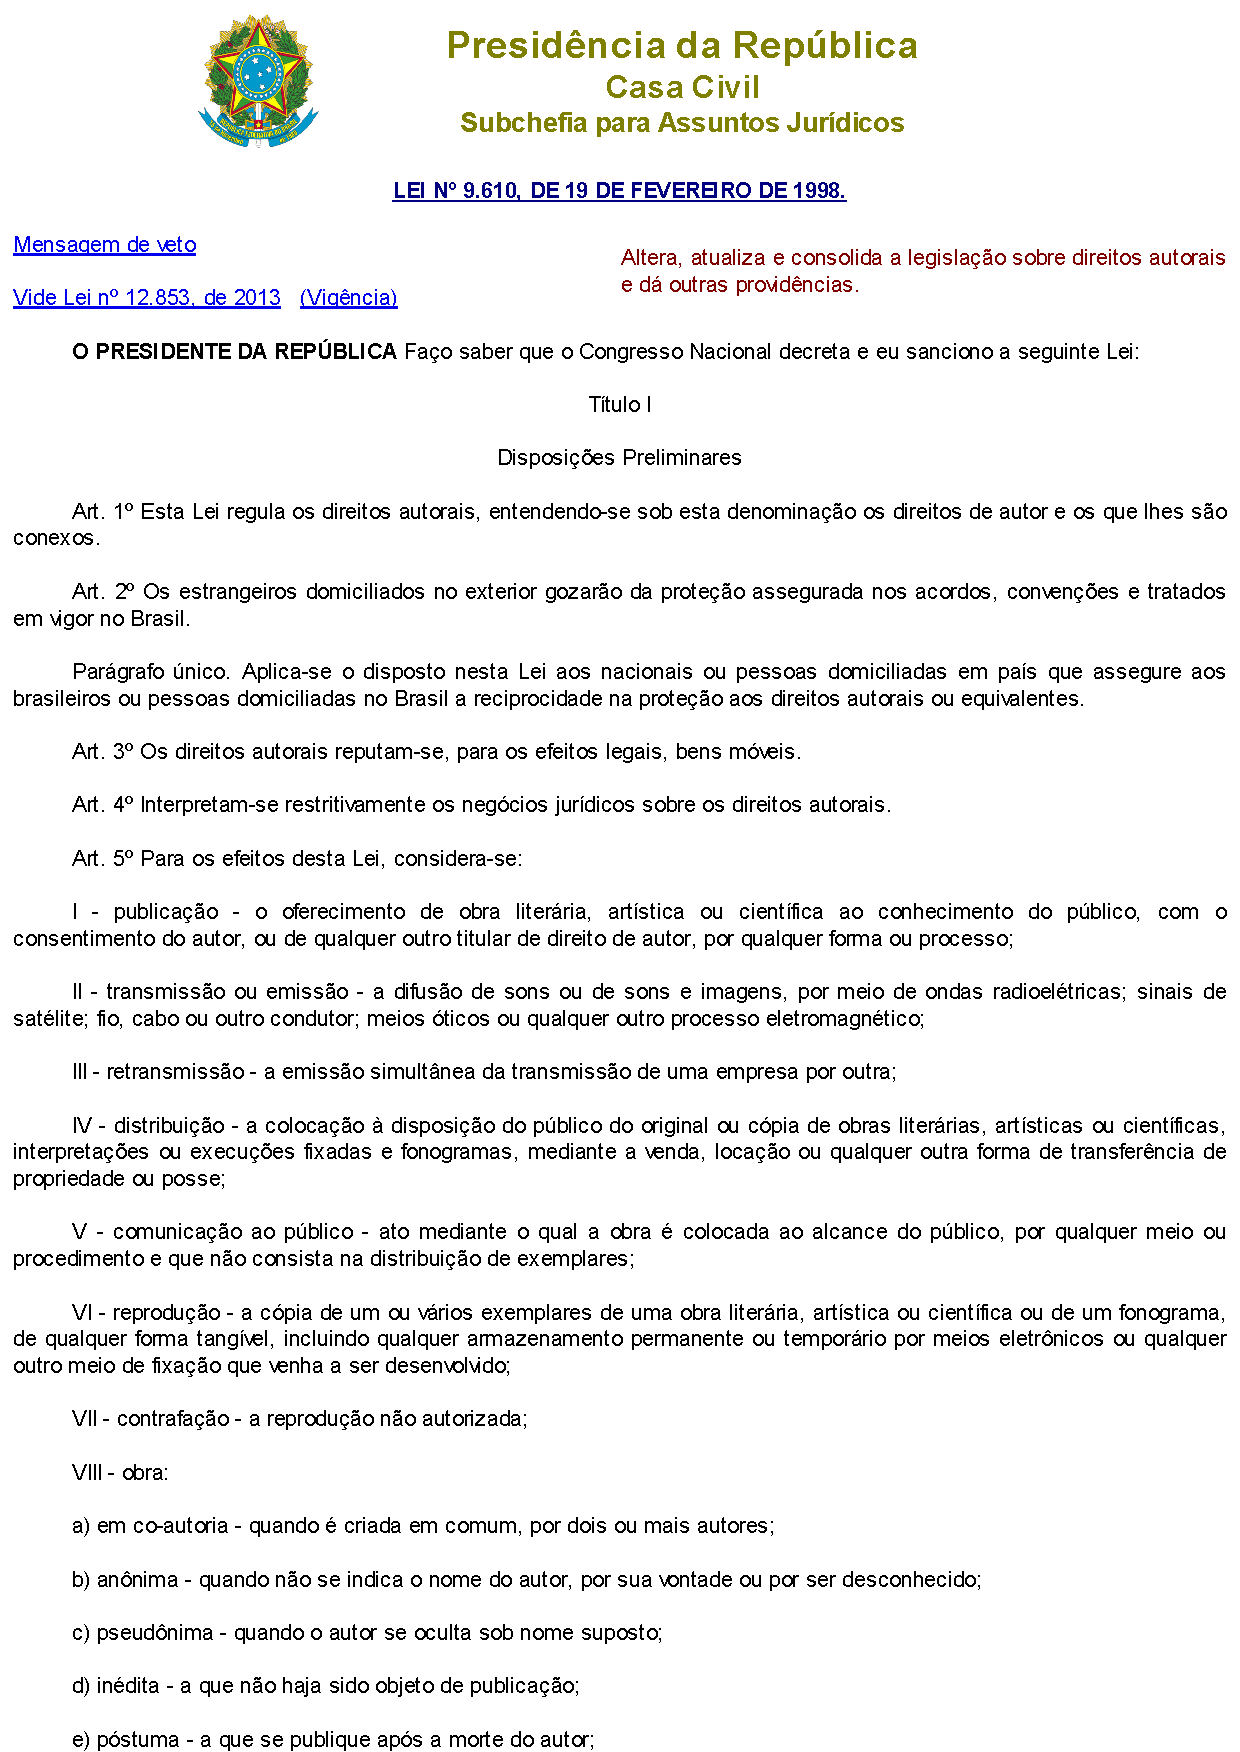
\includegraphics[width=\textwidth]{./PosTexto/Ilustracoes/lei-n9610-p1}}%% Imagem (Dimensões e localização)

% \centerline{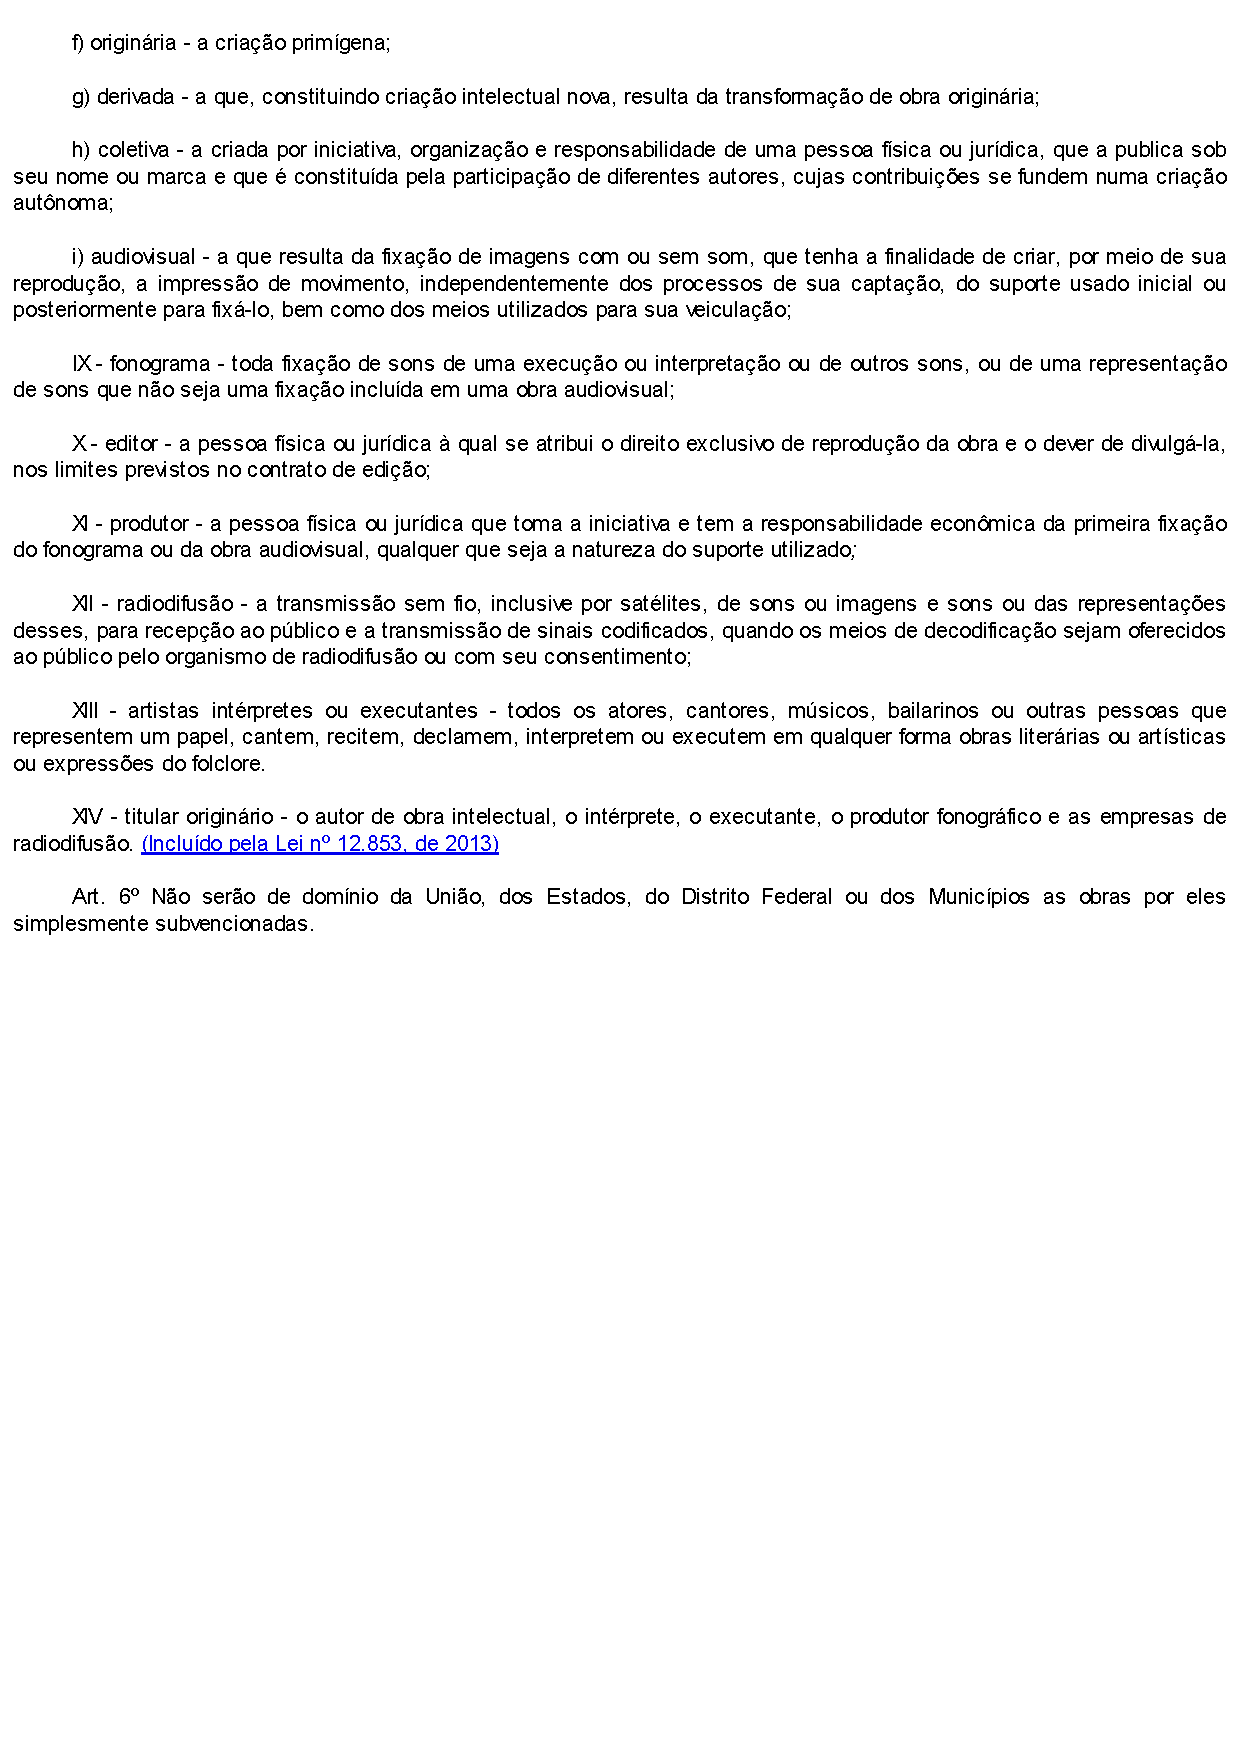
\includegraphics[width=\textwidth]{./PosTexto/Ilustracoes/lei-n9610-p2}}%% Imagem (Dimensões e localização)
%% Anexo - Comente para remover este item
%  %\include{./PosTexto/anexob}%% Anexo - Comente para remover este item
\end{arquivosdeanexos}%% Não comente esta linha
%%%%%%%%%%%%%%%%%%%%%%%%%%%%%%%%%%%%%%%%%%%%%%%


%%%%%%%%%%%%%%%%%%%%%%%%%%%%%%%%%%%%%%%%%%%%%%%
%% Índice
%%
\incluirindice%% Comente para remover este item
%%%%%%%%%%%%%%%%%%%%%%%%%%%%%%%%%%%%%%%%%%%%%%%

%% Fim do documento
\end{document}%% Não comente esta linha
%%%%%%%%%%%%%%%%%%%%%%%%%%%%%%%%%%%%%%%%%%%%%%%